\documentclass{book}
\usepackage{graphicx}
\usepackage{amsmath}
\usepackage{esint}
\usepackage{mhchem}
\usepackage{braket}
\usepackage{appendix}
\usepackage[export]{adjustbox} 
\usepackage{wrapfig}
\usepackage{listings}
\usepackage{color}
\usepackage{url}
\usepackage[a4 paper, total={8in, 8in}]{geometry}

\title{EGB241: Magnetics and Machines}
\author{Lachlan Dunne}
\date{\today}


\begin{document}

\chapter{Assessment:}

\begin{enumerate}
	\item \textbf{Quizzes:} 1 (20/04/23),2 (11/05/23), 3 (01/06/23)
	\item \textbf{Group Design:} Weighting: 0.2. First task is a computing design task that will be used to help with design work.
\end{enumerate}

 

\begin{itemize}

	\item \begin{figure}
			\centering
			\includegraphics[width=0.7\linewidth]{../../EGB240/Notes/assignment_screenshots/packing_factor}
			\caption{Packing Factor: DC Motor Winding}
			\label{fig:packingfactor}
		\end{figure}
\end{itemize}
\subsection{Materials}



\chapter{Content}

\section{Week 1: Review}

\subsection{Phasors and Complex Numbers}

\begin{align*}
	e^{j\theta} &= 1+ j \theta + \frac{j^2\theta^2}{2!} + \frac{j^3 \theta^3}{3!}+... \\
	e^{j \theta} &= cos \theta + j sin \theta \\
	cos\theta &= \frac{e^{j\theta} + e^{-j\theta}}{2} \\
	sin\theta &= \frac{e^{j\theta} - e^{-j\theta}}{2j} \\
	(cos\theta + jsin\theta)^n &= cos(n\theta)  + jsin (n\theta)
\end{align*}
Phasors and complex numbers are used very widely in electrical engineering to represent AC voltages and currents. We will enumerate the rules of phasor mathematics, and a few helpful trigonometric identities. There are a wider variety of trig identities on the cheat sheet in your hard drive.

\begin{enumerate}
	\item \textbf{Complex Forms:}
	\begin{align*}
		z &= a+bj \text{ (Cartesian Form)}\\
		z &= r(cos\theta + jsin\theta) = r\angle \theta \text{ (Polar Form)} \\
		|z| &= r = \sqrt{a^2 + b^2} \\
		a &= rcos\theta \\
		b &= rsin\theta \\
		tan\theta &= \frac{b}{a}
	\end{align*}
	\item \textbf{Phasors and Conjugates:} It is straightforward to show that:
	\begin{align*}
		r\angle -\theta &= rcos(-\theta) + jsin(-\theta) \\
		&= rcos(\theta - j sin \theta) \\
		&= \bar{z} \\
	\end{align*}
	Taking the negative angle of a phasor is equivalent to taking the complex conjugate.
	\item \textbf{Multiplication, division, addition in Polar Form}
	\begin{align*}
		z_1 z_2 &= r_1 r_2 \angle (\theta_1 + \theta_2) \\
		\frac{z_1}{z_2} &= \frac{r_1}{r_2} \angle (\theta_1 - \theta_2)
	\end{align*}
\end{enumerate}

\subsection{Mechanics}

In this section I will briefly list the mechanical relationships used to describe machines, this will serve as a very brief review of fundamental relationships in machine dynamics.

\begin{enumerate}
	\item \textbf{Angular Displacement:} Angular Displacement is a measurement of displacement from some specified reference point, measured in radians. This concept can be expanded into three dimensions for control applications:
	\begin{align*}
		(\theta_x, \phi_y, \psi_z) = \text{(Roll, Pitch, Yaw)}
	\end{align*} 
	\item \textbf{Angular Acceleration and Velocity:} As with traditional displacement, we can represent angular acceleration and vecloity in terms of the rate of change of velocity and position.
	\begin{align*}
		\omega_{x,y,z} &= \dot{\theta}, \dot{\phi}, \dot{\psi}
	\end{align*}
	More simply put, we typically decribe these quantities in terms of general solutions to differential equations, those being:
	\begin{align*}
		\omega &= \omega_0 + \alpha t \\
		\theta &= \theta_0 + \omega_0 t + \frac{1}{2}\alpha t^2 \\
		\omega^2 &= \omega_0^2 + 2 \alpha(\theta - \theta_0) 
	\end{align*}
	\item \textbf{Linear Relationships between Angular and Linear Quantities:}
	Velocity is simply defined as the rate of change of position over some time $t$. We know in angular motion we can determine the tangential velocity $v_t = ds/dt$, where $s$ is defined via the circular path travelled about some rotational point, thus it is trivial to show:
	\begin{align*}
		v_t = \frac{ds}{dt} = r \frac{d\theta}{dt} = r\omega
	\end{align*}
	Thus, we can see that tangential (or 'linear') velocity is dependent upon $r$, and therefore it changes depdendent upon the distance from the axis of rotation. \newline
	
	Tangential acceleration is just as easily defined as:
	\begin{align*}
		a_t = \frac{dv}{dt} = r \frac{d\omega}{dt} = r \alpha
	\end{align*}
	\item \textbf{Torque:} Torque is generated when a force is applied perpendicular to some radius extending from a point of rotation. 
	\begin{align*}
		\tau = \vec{r}\vec{F} 
	\end{align*}
	Direction is a very important factor of this process.
	\item \textbf{Work:} In linear motion, work is defined as the application of force through a distance. Likewise, for rotational motion, work is defined as torque applied through an angle.
	\begin{align*}
		W &= \int_{\theta_i}^{\theta_f} = \tau d \theta \\
		W &= \tau \theta \text{ (Constant torque)}
	\end{align*}
	\item \textbf{Power:} Power is the rate of doing work, or the increase in work per unit time.
	\begin{align*}
		P = \dot{W}
	\end{align*}
	And can be measured in J$\cdot$s, W, foot-pounds per second or horespower. For linear motion, $P = F \dot{x} $, for rotational motion:
	\begin{align*}
		P &= \dot{W} = \tau \dot{\theta} = \tau \omega
	\end{align*}
	Which is very important in the case of electrical machinery as it describes the mechanical power on the shaft of a motor or generator.
	\item \textbf{Moment of Inertia:} The moment of inertia describes a bodies resistance to movement or lack of.  We can  use moment of inertia to find rotational kinetic energy $K = 1/2 I \omega^2$ as it relates the movement of mass and its velocity. We can evaluate the moment of inertia using calculus:
	\begin{align*}
		I = \int \rho r^2 dV
	\end{align*}
	This formula can be used to solve geometrically if the body is homogenous and isotropic (constant density, etc). We can also define the net work done by external forces in rotating a body via:
	\begin{align*}
		W = \frac{I}{2}(\omega^2 - \omega_0 ^2)
	\end{align*}
\end{enumerate}

\subsection{Rotational Mechanics}

	
\subsection{Inductance and Capacitance}

Within the study of electrical engineering, it is important to have a grasp of solutions to integro-dfferential equations, as they dictate the simplest circuit configurations. For example:

\begin{itemize}
	\item A simple RC circuit in series with a voltage source can be modelled via the differential equation:
	\begin{align*}
		\frac{dI(t)}{dt}(R) &= \frac{-1}{RC}\frac{dq_c}{dt} \\
		I_s(t) &= -\frac{v_0}{R} e^\frac{-t}{RC} = I_0 e^\frac{-t}{RC} \\
		I_C(t) &= \frac{I_sR-v_0}{R}e^{-t/RC}  \\
		V_C(t) &= I_s R - (I_s R - v_0 )e^{-t/RC}
	\end{align*}
	\item Likewise, a simple RL circuit has a natural (RL in series) general solutions of the form:
	\begin{align*}
		i_l(t) &= i_0 e^{-Rt/L} \\
		v_l(t) &= i_0 R e^{-Rt/L}
	\end{align*}
	And step responses (voltage input) with general form:
	
	\begin{align*}
		i_l(t) &= \frac{V_s}{R} - (\frac{V_s}{R} - i_0) e^{-\frac{Rt}{L}} \\
		v_l(t) &= (v_s - i_0 R)e^{\frac{-Rt}{L}}
	\end{align*}
\end{itemize}

Now, although the DC forms of these equations have nice general solutions, linear AC circuits have physical parameters that rely upon the frequency of the input signal, and thus require a different approach. One such approach is phasor analysis, Laplace transform approach, or state space analysis.

\begin{itemize}
	\item \textbf{Inductor Summary:} Inductor components are a consequence of \textbf{self-induction}, which occurs when in a conductor changing magnetic flux is induced through an area of space, Faraday's law states that the changing magnetic flux induces an electric field, and it Lenz's law states this field must be in opposition to the magnetic flux. We find that the flux is proportional to the magnetic field established which in turn is proportional to the current: ($\varepsilon = -N \frac{d\Phi_B}{dt} = -L\frac{dI}{dt} $). Thus we can derive the expression for voltage across an inductor with:
	\begin{align*}
		v_L(t) &= -N \frac{d\Phi_B}{dt} \\
		L &= N \frac{\Phi_B} {I} \\
		\Phi_B &= \frac{IL}{N} \\ 
		v_L(t) &= -L \frac{di(t)}{dt}
	\end{align*}
	Where the proportionality constant $L$, or the inductance, encapsulates the geometry and material parameters of our device. With a sinusoid input, it is rather trivial to define voltage for an inductor, if $v_L$ is the instantaneous drop across the inductor:
	\begin{align*}
		v- L \frac{di(t)}{dt} &= 0 \\
		L \frac{di}{dt} &= V_m sin(\omega t)\\
		i_L &= \frac{V_m}{L} \int sin(\omega t) dt = - \frac{V_m}{\omega t} cos(\omega t)\\
		i_L &= \frac{V_m}{\omega L} sin(\omega t - \frac{\pi}{2})
	\end{align*}
	From this, we note that current lags voltage by a phase of $\pi/2$. We can also see that the peak current is at $I_m = V_m / \omega L$. From this point we define the \textbf{inductive reactance}, which comes up often in phasor and frequency analysis:
	\begin{align*}
		X_L &= \omega L \\
		v_L &= V_m sin (\omega t) = I_m X_L sin (\omega t) \\ 
	\end{align*}
	Inductors \textbf{block high frequencies}. Physically this can be interpreted as a conseqence of Lenz's law. The induced emf in high frequency circuits should theoretically block high frequency signals. 
	\item \textbf{Capacitor Summary:} Capacitors in an AC circuit are modelled very similarly to inductors. First, we derive an expression for instantaneous capacitance accross the capacitor:
	\begin{align*}
		v_c &= V_m sin(\omega t) \\
		i_c &= \frac{dQ}{dt} = \omega CV_m cos(\omega t) \\
		i_c &= \omega C V_m sin(\omega t + \frac{\pi}{2})
	\end{align*}
	
	Similarly to inductors, we see there is a phase difference between current and voltage. Thus for sinusoidally varying emf, the current always leads the voltage by $\pi/2$.  We can see that the peak current in the circuit is:
	\begin{align*}
		I_m &= \omega C V_m = \frac{V_m}{X_c} \\
		X_c &= \frac{1}{\omega C} \\
		U_C &= \frac{Q^2}{2C} = \frac{1}{2}QV = \frac{1}{2}CV^2
	\end{align*}
	Capacitors \textbf{block DC signals} (high reactance at low frequencies) in AC circuits.
	\item \textbf{Phasor Summary of capacitors and inductors:} We can derive analytical relations between capacitors, resistors and inductors, but it is easier and more intuitive to consider the \textbf{phasor diagram approach:} We know that the current in capacitors leads the voltage by $\pi/2$, that currents in inductors lag the voltage by $\pi/2$. Effectively, voltages in inductors and capacitors are $\pi$ radians \textbf{out of phase}. In an \textbf{RLC} circuit application, the current is the same across all three circuit elements. Therefore, in the KVL states:
	\begin{align*}
		v &= v_r + v_c + v_l \\
		V_m &= I_m \sqrt{R^2 + (X_L + X_C)^2} \\
		Z &= \sqrt{R^2 + (X_L - X_C)^2} \\
		tan \phi &= \frac{X_L-X_C}{L}
	\end{align*}
\end{itemize}

\subsection{Power in AC}

As currents and voltages vary with time, power in AC is a bit more slippery to define. We know that:
\begin{align*}
	P = iv = i^2 R
\end{align*}

However this only describes instantaneous power, and it is much more practical to define:
\begin{align*}
	P_{av} &= \frac{1}{2} I_m V_m cos \phi \\
	P_{av} &= I_{rms} V_{rms} cos \phi 
\end{align*}

However, even further we can define real, reactive and apparent powers supplied to a load via a \textit{power triangle}:


\subsection{Power Factor Calculations:}

Power factor, is the ratio of working power (typically measured in kW), to apparent power, measured in kVA. Apparent power is also known as demand, and is the measure of power drawn to run machinery and equipment over some period of time, measured in kVA. 

\textbf{The BEER Analogy:}
\begin{itemize}
	\item \textbf{Liquid Beer} is active power (kW). This is the useful power, this is the energy doing work per unit time.
	\item \textbf{Foam Beer} is the reactive power (kVAR). The foam is the 'wasted' power, the energy that isn't doing any work, such as the production of heat or vibration.
	\item \textbf{The pint} is apparent, or demand power. This is the total power being delivered. 
\end{itemize}

In all but the most ideal cases (such as superconductors), there will be loss in the circuit.  This is where the power triangle is helpful.
\begin{figure}[h]
	\centering
	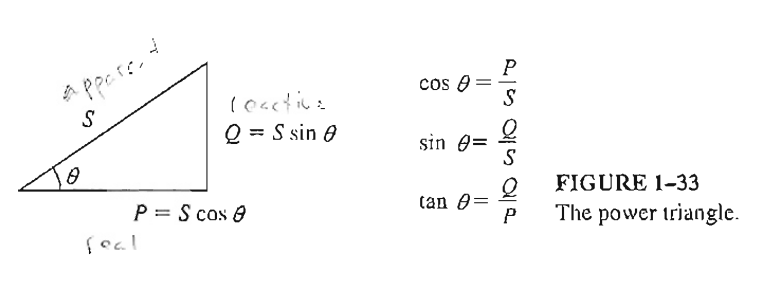
\includegraphics[width=0.4\linewidth]{Screenshots/power_triangle}
	\caption{Power Triangle}
	\label{fig:powertriangle}
\end{figure}
\subsection{Faradays Law}

Faraday's law describes the voltage induced in a closed current loop as the magnetic flux through said loop changes in time. We can generalize Faraday's law to integral form, expressing a more far-reaching concept in electromagnetism:

\begin{align*}
	\varepsilon = \oint (\vec{v} \times \vec{B}) \cdot d \vec{l}
\end{align*}

\textbf{Expand upon}
\section{Week 2: Magnetic Circuits}

We shall see that certain configurations of magnetic materials (in approximately circuit form) when an external magnetic field, most commonly provided (in engineered applications), by a coil of current carrying wire, can be approximated with DC circuit analysis techniques. I will enumerate the concepts and their direct analogs to Ohms law:

\begin{enumerate}
	\item \textbf{Magnetomotive Force:} Magnetomotive force is derived from the magnetization caused from an external source in a magnetic circuit, which may be a permanent magnet or solenoid wrapped around the base of a magnetic material. Its behaviour is analogous to voltage.

	\item \textbf{Magnetic Flux:} Magnetic flux is the total magnetic field density permeating through a material. Magnetic flux will generally travel through the most permeable material available. Its behaviour is analogous to current. 
	\item \textbf{Reluctance:} Reluctance of a material is best defined in terms of electrical resistance. It is inversely dependent on relative permeability.  
\end{enumerate}

\subsection{Ohms Law: Electric and Magnetic}

Traditionally, Ohms law is widely applicable in DC circuit theory. We can easily derive Ohms law by considering a differential circuit element with area $A$, and a distance of seperation $dy$. First, we define a few relations:

\begin{itemize}
	\item Voltage, in this circumstance, is defined as the amount potential energy a point charge has when seperated by $dy$ from a lower potential. We describe this seperation by the electric field $\vec{E}$. Thus, $V=|\vec{E}| d\vec{y}$.
	\item Current density describes the net movement of charge in a circuit elements area, due to the driving force of the electric field $\vec{E}$. Furthermore, we define a the materials conductivity $\sigma$, which is a atomic property of the material in which the current is flowing. The equation described is $\vec{J} = \sigma \vec{E} = n q v_d$, where $v_d$ is drift velocity, a statistical description of the net movement of a charges $nq$ in a conductor. This parameter is dependent on temperature.   
	\item Finally, the Resistance of a material. $R$, is given by: 
	\begin{align*}
		R = \frac{L}{A \sigma} = \frac{L \rho}{A}
	\end{align*}
	Where $\rho$ is the inverse of conductivity, $\sigma$.
\end{itemize}

Using these three equations, we can substitute $|\frac{J}{\sigma}| =J\rho=|\vec{E}| $ into $V = |\vec{E}| dy$. Which we get:
\begin{align*}
	J \rho d\vec{y} =V 
\end{align*}

We can derive from current density current, given by $\frac{J}{A} = I$. Thus, substituting this into the above equation:
\begin{align*}
	\frac{I}{A} \rho d\vec{y} &= V \\
	V&= IR \text{ (Ohms Law)}
\end{align*}
We use Ohms law to model typical electrical circuits. We now aim to replicate Ohm's law for magnetic circuits
\begin{align*}
	\mathsf{F} &= NI = \Phi \mathsf{R} = \frac{\Phi d}{\mu A} = \vec{H} d\\
	\mathsf{R} &= \frac{d}{\mu A} \\
	\Phi &= \frac{NI}{\mathsf{R}} = \vec{B} A \\
	\vec{B} &= \mu_r \vec{H}
\end{align*}



The three above equations are derived from $|\vec{B}| = \mu |\vec{H}|$. Magnetic circuits, (for some limited geometries), behave similarly to traditional DC circuits, which some assumptions, of course (such as negligible leakage flux). Thus, we can apply Ohms law for magnetic circuits in the same way we apply it for electrical circuits. 

\begin{figure}[h]
	\centering
	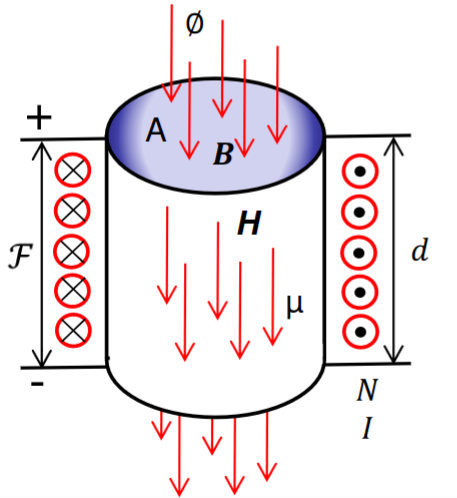
\includegraphics[width=0.2\linewidth]{Screenshots/magnetic_OHMS}
	\caption{Magnetic Element}
	\label{fig:magneticohms}
\end{figure}

\begin{itemize}
	\item \textbf{Equivalent Reluctance:} Reluctance can be combined in parallel and in series, in the same way that resistances are.
	\item \textbf{Kirchoffs Current Law for Flux:} 
	\begin{figure}[h]
		\centering
		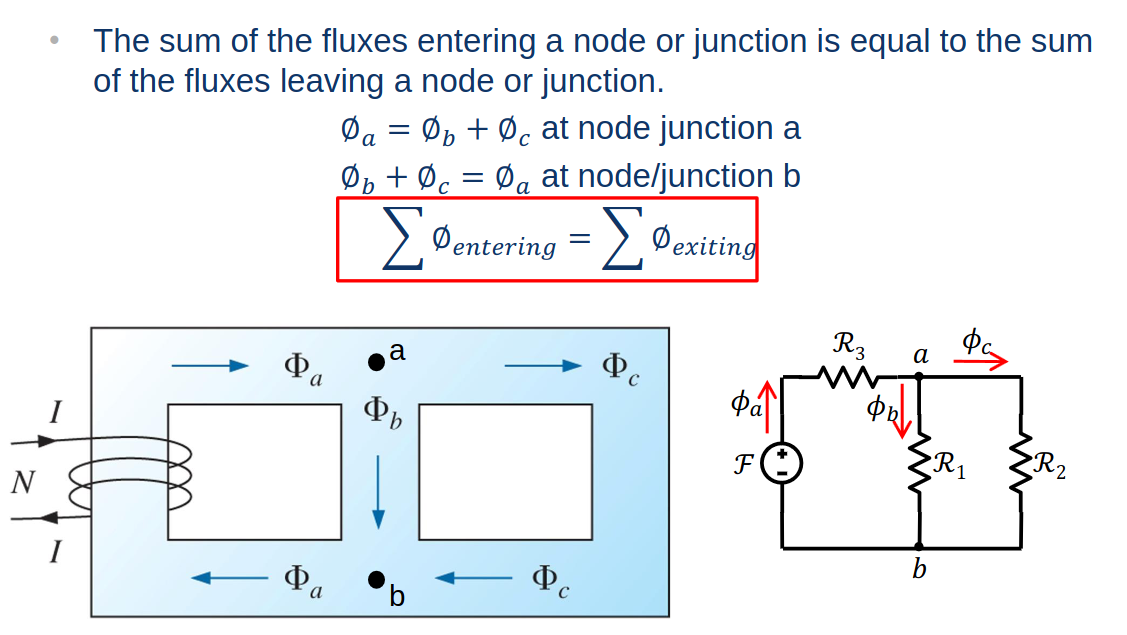
\includegraphics[width=0.3\linewidth]{Screenshots/KCL_flux}
		\caption{KCL for Flux}
		\label{fig:kclflux}
	\end{figure}
	\newpage
	\item \textbf{Kirchoffs Voltage Law for Magnetomotive Forces:}
	\begin{align*}
		\sum mmf &= \sum F
	\end{align*}
	\begin{figure}
		\centering
		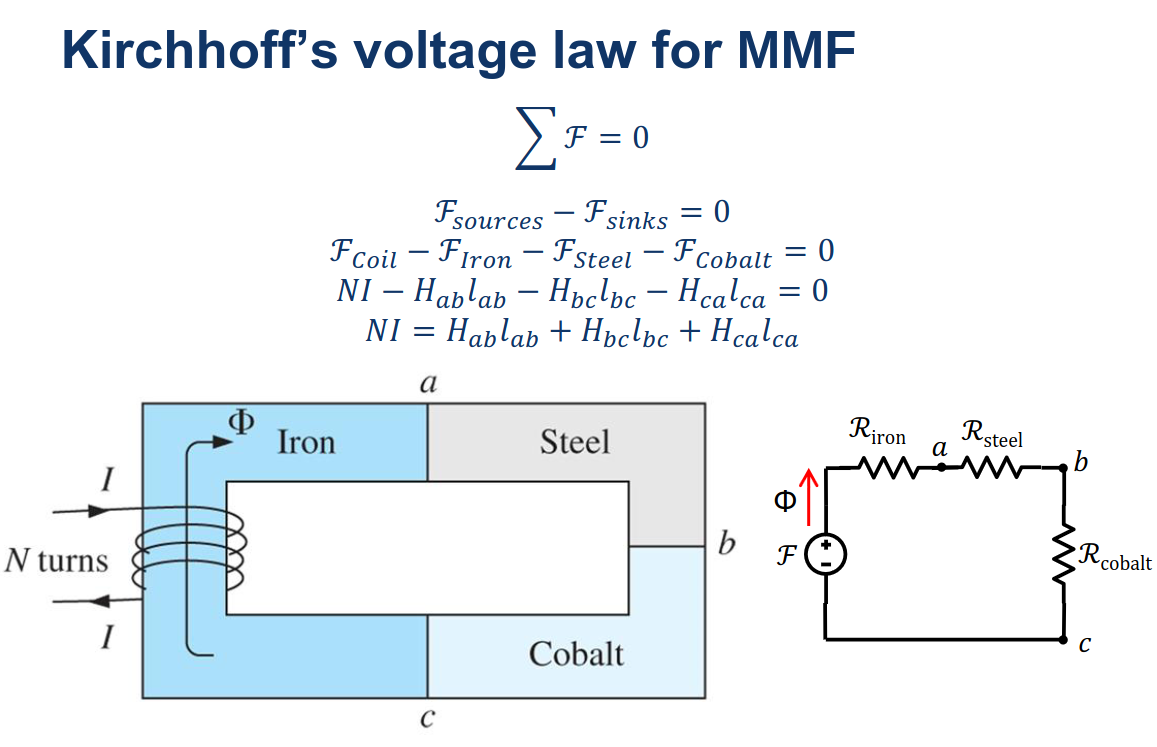
\includegraphics[width=0.3\linewidth]{Screenshots/KVL_MMF}
		\caption{KCL for Magnetomotive Forces}
		\label{fig:kvlmmf}
	\end{figure}
\end{itemize}

\subsection{Reluctance in Detail:}

Reluctance is the magnetic analog of resistance, and it defines how well magnetic fields permeate in differering media (as opposed to current in traditional DC circuits). As we see by the equation:
\begin{align*}
	R_{B} &= \frac{d}{\mu A} = \frac{d}{\mu_0 \mu_r A}
\end{align*}

With an increase in permeability $\mu$, the smaller the nominal values of $R_B$. In many ferromagnetic materials, which are used due to their magnetized domains in many machine applications (which also adds \textbf{non-linearities} from hystersis), relative permeability is much higher than that of parramagnetic and diamagnetic materials. The calculation of reluctance assumes a certain mean path length and cross-sectional area for the core. These assumptions aren't great, particularly at edges where leakage flux occurs.

\subsection{MMF}

The magnetomotive force is defined as \textbf{the driving force that causes flux to form in a magnetic field}. Repeating our equation above:
\begin{align*}
	\mathsf{F} &= NI = \Phi \mathsf{R} = \frac{\Phi d}{\mu A} = \vec{H} d = \frac{\vec{B} l_e}{\mu_{eff} \mu_0}\\
\end{align*}
These equations have been derived from Amperes law and assumes that the coils length is much larger than its diameter. 

Just as the permittivity of free space and certain materials dictates the behaviour of materials, the permeability of materials (be it air, or ferromagnetic materials, etc...) deeply effects the behaviour of the magnetomotive force in magnetic circuits. We know however, ferromagnetic materials are certainly non-linear, and thus cause grief in particular applications. 



\subsection{B-H Curves:}
A B-H curve is an important graphical representation of a magnetic materials permeability. It graphs the magnetic field $\vec{B}$ and its intensity $H$ an, by observation of these curves we see that they are non-linear. Recall that the magnetization value $H$ is related to the magnetic field $\vec{B}$ via the relationship:
\begin{align*}
	\vec{B} &= \mu H \\
	H &= \frac{NI}{l_c} = \frac{\mathsf{F}}{l_c}
\end{align*}
\begin{figure}[h]
	\centering
	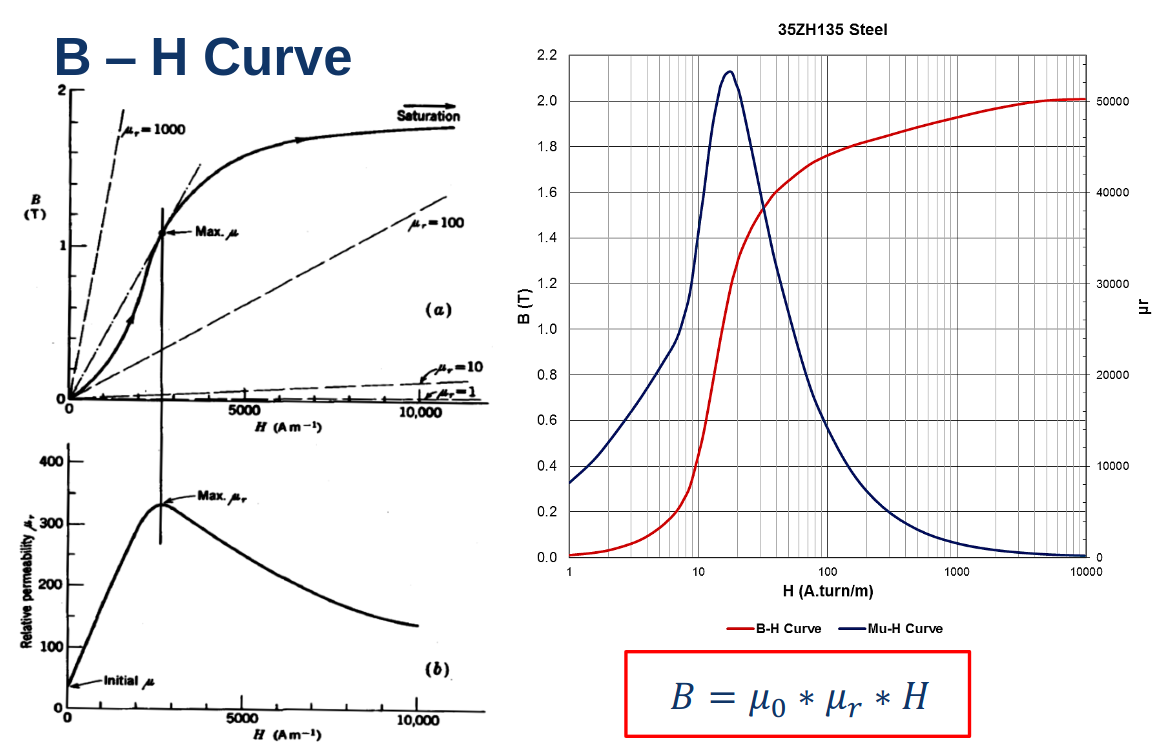
\includegraphics[width=0.4\linewidth]{Screenshots/BH_curve}
	\caption{BH and $\mu$ H curve}
	\label{fig:bhcurve}
\end{figure}
 Note that the magnetic field $\vec{B}$ depends on the product of the permeability free space $\mu_0$, $\mu_r$ and $H$. Some key interpretations we can take away from the diagram:
 \begin{itemize}
 	\item  $\vec{B}$ on the y-axis is plotted against \textbf{magnetizing intensity $\vec{H}$}, which is essentially a measurement of work required to magnetize the material.
 	\item The \textit{knee} point, or turning point of the BH curve corresponds to the maximum value of permeability $\mu$
 	\item The region before the knee point is called the unsaturated region. At this point, flux changes rapidly, and the core is said to be unsaturated.
 	\item The region beyound the knee point is called the saturated region. Flux plateaus at this point. Note that the flux is linearly related to the applied magnetomotive force $NI$ in the saturated region.
 	\item The \textbf{core loss} is a parameter used to measure the energy dissapated during a 'cycle', which can be found as the area bound by the BH curve.
 \end{itemize}
	
\textbf{Permeability $\mu$ and mmf $\mathbf{F}$}
Some other important parameters to consider when analyising the $B-H$ properties of certain materials is the non-linear characteristics and their dependency on:
\begin{enumerate}
	\item Temperature
	\item Frequency
	\item Stress and strain on the material
	\item Magnetic Field intensity $H$
	\item Direction of rolling or gain of the material
	\item And more.
\end{enumerate}
\begin{figure}[h]
	\centering
	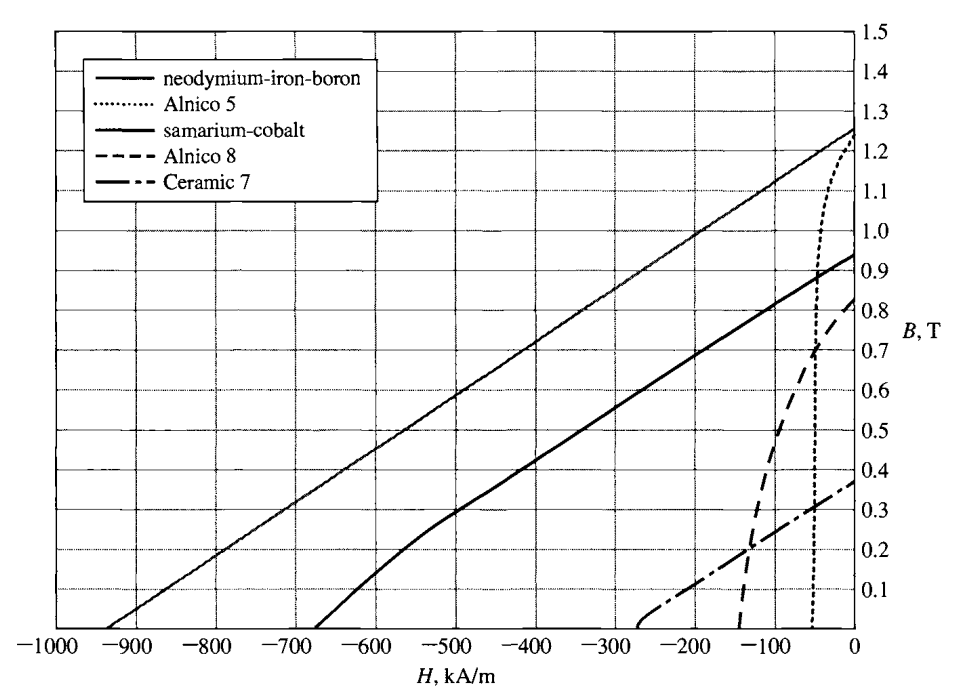
\includegraphics[width=0.5\linewidth]{Screenshots/Common_BH_Curves}
	\caption{Common BH-Curves}
	\label{fig:commonbhcurves}
\end{figure}

 
 \subsection{Flux Linkage}
 
 
 \textbf{Previous understanding:}
 Flux linkage is a result of Gauss's law in $2D$. If we know the flux through one loop, and a second loop is closly spaced, and of the exact same geometry, we can use this symmetry to write an expression for the equivalent flux, $\Phi_{total} \approx N \Phi_1$. From here we define flux linkage $\lambda$ as the number of loops multiplied by the total flux linking them.
 \begin{align*}
 	\lambda &= N \Phi_{total} = N^2 \Phi_1
 \end{align*}
 
 \textbf{Updated Understanding:}
 
 When a magnetic field varies with time, an electric filed is produced in space as determined by \textit{Faraday's law:}
 \begin{align*}
 	\oint_C \vec{E} \cdot d\vec{s} = \frac{-d}{dt} \int_{S} \vec{B} \cdot d\vec{a}
 \end{align*}
 
 This equation states that the closed contour $C$ is equal to the time rate of change of the magnetic flux linking (i.e, passing through that contour). In magnetic structures with windings of high electrical conductivity, such as solenoids, it can be shown that the $\vec{E}$ field in the wire is exteremely small and can be neglected. In addition to this, the flux on the right hand side of Faraday's law is dominated by the core flux $\Phi$. Since the winding (and hence the contour C) links the flux $N$ times, we can simplify the integrals and arrive at:
 
 \begin{align*}
 	e = N\frac{d\Phi}{dt} = \frac{d\lambda}{dt}
 \end{align*}
 
 Where the flux linkage is defined as $\lambda = N \Phi$, and is measured in units of webers (or weber-turns). We can also define the inductance in terms of flux linkage over current, $L = \frac{\lambda}{I}$. For a typical, ideal inductor, (which was discussed in the review section), we defined the voltage accross it as:
 \begin{align*}
 	v(t) = L \frac{di(t)}{dt}
 \end{align*}
 
 And therefore:
 \begin{align*}
 	v(t) = \frac{\lambda}{I} \frac{di(t)}{dt}
 \end{align*}
 
 
 \subsection{Inductance as a ratio of Flux Linkage}
 
 Inductance can be defined as the ratio of flux linkage $\lambda$ to the generating current $I$ generating the flux. It is measured in units: H, Wb/A. 
 \begin{align*}
 	L = \frac{\lambda}{I} = \frac{N \phi_{total}}{I} = \frac{N^2 \phi_1}{I}
 \end{align*}
 For a coil wound around a core:
 \begin{align*}
 	\phi_{total} &= \frac{\mathsf{F}}{\mathsf{R}} = \frac{NI \mu A}{d} \\
 	L &= \frac{N^2 \mu A}{d} \\
 	L &= \frac{N^2}{R}
 \end{align*}
 \subsection{Faradays Law}
 
 Faradays law forms the basis of electromagnetic induction. It is formulated in terms of a rather simple differential equation:
 
 \begin{align*}
 	\varepsilon &= - \frac{d\Phi_B}{dt}  \\
 	\nabla \times \vec{E} &= - \frac{d\vec{B}}{dt}
 \end{align*}
 
 This equation links the electrical and magnetic field and is vital when considering modern machinery. We can also relate a the new term, \textbf{flux linkage} to Faradays law (in true engineering fashion): If there are $N$ turns in a coil of wire, the total voltage on the coil is the sum of induced voltages:
 \begin{align*}
 	\varepsilon_{ind} &= \sum_{i=1}^N \varepsilon_i \\
 	&= \sum_{i=1}^N \frac{d (\Phi_{Bi})}{dt} \\
 	&= \frac{d}{dt} (\sum_{i=1} ^N \Phi_i) \\
 	\varepsilon_{ind} &= \frac{d \lambda}{dt} \\
 	\lambda &= \sum_{i=1}^{N} \Phi_i 
 \end{align*}
 
 \textbf{Motional EMF:} Arises from Faraday's law, and is most simply illustrated with a linear DC machine. Imagine a closed circuit, with some voltage source, internal resistance and a slide bar, allowing the circuits total area to increase. When in a magnetic field, clearly there is some non-zero flux, which can be expanded via work done on the slide bar. We have derived an equation for the force exerted on some length of current-carrying wire in a magnetic field in Surways textbook (page 810):
 \begin{align*}
 	F &= I l\times \vec{B}
 \end{align*}
 
 Our simple circuit's behaviour is summarized by:
 
 \begin{enumerate}
 	\item A force $F_{app}$ is applied in the direction of motion; $F_{net}$ is in the direction of motion.
 	\item Acceleration $\vec{a} = 	F_{net} / m $ is positive, so the bar speeds up.
 	\item The voltage $e_{ind} = v \vec{B}l$ increases, and so $i= (\varepsilon - v_s) / R$ increases. 
 	\item The induced force $F_{ind} = i l\vec{B}$ increases until $|F_{ind}| = |F_{load}|$ at a higher speed $v$.
 	\item An amount of mechanical power equal to $F_{ind}v$ is now being converted to electric power $e_{ind}i$, and the machine is acting as a generator. 
 \end{enumerate}

\subsection{Real and Reactive Power:}

In AC circuits, we have to model the transportation of power in a more involved manner than DC circuits. If we have a simple source-load circuit, with $v(t)= \xrightarrow{} V \angle 0$, $I= I \angle -\theta$ and $Z=Z\angle \theta$, as shown in the diagram below:
\begin{figure}[h]
	\centering
	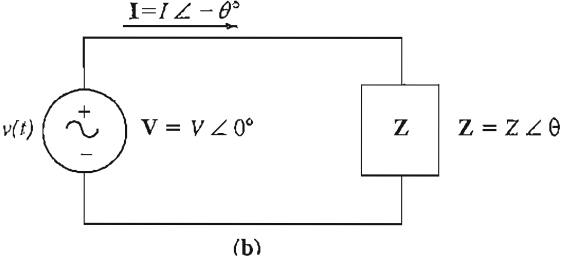
\includegraphics[width=0.3\linewidth]{Screenshots/v_load}
	\caption{Simple AC Circuit}
	\label{fig:vload}
\end{figure}

Where the RMS voltage is $\sqrt{2}V cost \omega t$, and the resulting current flow is $\sqrt{2}Icos(\omega t - \theta)$ where $I$ is the rms value of the current flowing through the load. The instantaneous power supplied to this load at any time $t$ is:
\begin{align*}
	p(t) = v(t)i(t) = 2VI cos(\omega t)cos(\omega t - \theta)
\end{align*}

Where $\theta$ is the impedance angle of the load. For \textbf{inductive} loads, the impedance is positive, and the current waveform lags the voltage waveform by $\theta$ degreees. The instantaneous power would be defined as the product of the two waveforms, the magnitude clearly determined by the overlap of the waveforms at any given point.
\begin{align*}
	p(t) = v(t)i(t) = 2VIcos \omega t cost(\omega t - \theta)
\end{align*}

Application of trigonometric indentities yields an expression of the form:
\begin{align*}
	p(t) = VI cos\theta(1+cos 2 \omega t) + VI sin\theta sin2\omega t
\end{align*}
The first term representing the power supplied by to the load by the component of current that is \textit{in phase} with the voltage. Software/graphical analysis of power makes it much more simple.

\subsection{Impedance Angle, Current Angle, and Power}

I thought that it is worth mentioning that \textbf{inductive loads} are loads with positive impedance angles, as inductors have positive reactance. If this is the case, the phase angle of the current flowing through the load will lag the phase angle of the voltage across the load by $\theta$:
\begin{align*}
	I = \frac{V}{Z} = \frac{V\angle 0}{|Z| \angle \theta} = \frac{V}{|Z|} \angle -\theta
\end{align*} 
Therefore, if the impedance angle $\theta$ is positve, the \textbf{reactive power} consumed by the load is \textbf{positive}.
In contrast, \textbf{capacitive loads} have a negative impedance angle $\theta$, since the reactance of the capacitor is negative. If the impedance angle $\theta$ of a load is negative, the phase angle flowing through the load will lead the voltage by $\theta$ and the \textbf{reactive power, Q, consumed by the load will be negative}.

\subsection{Electromechanical Circuits and Energy Relations}

There are a variety of ways to develop an understanding of the functioning of electromechanical systems. In this section, we are concerned with the electromechanical-energy conversion process, which takes place through the medium of the electric or magnetic field of a conversion device.  We will look into some devices, for example:

\begin{itemize}
	\item \textbf{Transducers:} Microphones, pickups, sensors, loudspeakers etc
	\item \textbf{Force-Producing Devices:} Solenoids, relays and electromagnets. 
	\item \textbf{Continuous Energy-Conversion Equipment}
\end{itemize}

We know that the Lorentz force law describes the force $\vec{F}$ on a particle of charge $q$, in couloumbs, $\vec{E}$ in volts per meter, and $\vec{B}$ in teslas. 

\begin{align*}
	\vec{F} = q(\vec{E}+ \vec{v} \times \vec{B})
\end{align*}

In situations where large numbers of charged particles are in motion, it is convenient to write the above in terms of charge density $\rho$, (C $\cdot$ m$^{-3}$)

\begin{align*}
	\vec{F}_v = \rho (\vec{E} + \vec{v} \times \vec{B})
\end{align*}

Where the subscript is indictative of \textit{force density}. In order to show the following relation, a fair bit of complex physics will be skipped. For currents flowing in conductive media, we can rewrite the function above in terms of \textit{current density:} $J=\rho \vec{v}$, which has units of amperes per square meter. The magnetic system force density can be rewritten as:
\begin{align*}
	\vec{F}_v = \vec{J} \times \vec{B}
\end{align*}

The following approach is said to be valid, when (conceptually, at least), we can seperate the loss mechanism from the energy-storage mechanism. Simply put, we write a conservation of energy equation to model the electro-mechanical operation of the machine. 

\begin{figure}[h]
	\centering
	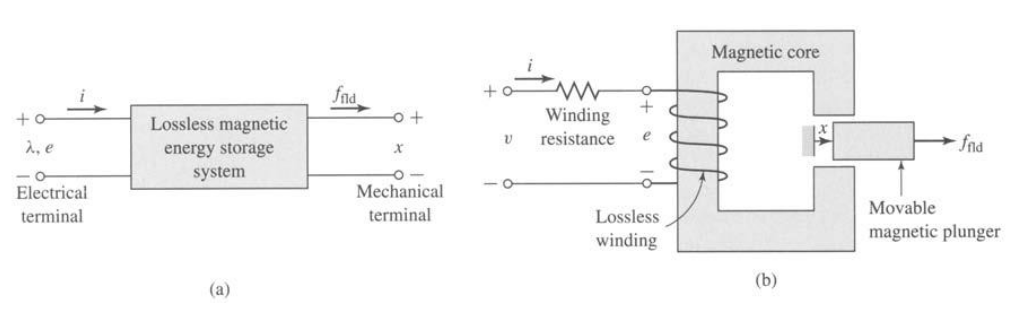
\includegraphics[width=0.4\linewidth]{Screenshots/electromech_model}
	\caption{(a) Magnetic-field electromechanical-energy-conversion deive (b) simple force-producing device}
	\label{fig:electromechmodel}
\end{figure}

As we assume the energy-storage system to be effectively lossless, we can write that the time rate of change of $W_{fld}$, the stored energy in the magnetic field, is equal to the electric power input (given by the product of terminal voltage and current) less the mechanical power output of the energy storage system.

\begin{align*}
	\frac{dW}{dt} = ei - f_{fld} \frac{dx}{dt}
\end{align*}

We can recognise that for our system in figure \ref{fig:electromechmodel}, we can write the voltage at the terminals of our lossless winding as:

\begin{align*}
	e = \frac{d\lambda}{dt}
\end{align*}

Multiplying by dt, we find:

\begin{align*}
	dW_{fld} = i d\lambda - f_{fld} dx 
\end{align*}

Thus, at the cost of detailed explanation of the force producing mechanism, this equation allows us to approximately model the behaviour of complex electro-magnetic systems. This also may allow one to approximate system losses, in the case where $dW$, $id\lambda$ and $fdx$ are observable values.  We can also determine the energy density of the system via the relation:

\begin{align*}
	W_{fld} = \frac{1}{2} L(x)i^2
\end{align*}

\textbf{Experimental Methods}

From the above relation, one can derive the useful relations from the system:

\begin{align*}
	dW_{fld} (\lambda, x) = \frac{\delta W_{fld}}{\delta \lambda}|_{x} d \lambda + \frac{\delta W_{fld}}{\delta x}|_{\lambda} dx
\end{align*}

We know that $\lambda$ and $x$ are independent variables, so  must be equal for values of $d\lambda$ and $dx$. Therefore, we can write:

\begin{align*}
	i &= \frac{\delta W(\lambda, x)}{\delta \lambda}|_x \\
	f_{fld} &= -\frac{\delta W_{fld}(\lambda, x)}{\delta x}|_\lambda
\end{align*}

In this case, we are able to determine either current $i$ on the system by varying the magnetic flux linkage $\lambda$ while holding position constant, and the force on the system by varying position $x$ whilst holding $\lambda$ constant. In any case, we are most likely to perform the latter.

\textbf{Torque}

For a system with a rotating mechanical terminal, the variables become the angular displacement $\theta$ and torque $\tau_{fld}$. Thus, writing a conservation equation yields:

\begin{align*}
	dW(\lambda, \theta) = i d\lambda - T_{fld} d\theta
\end{align*}

By analogy, we can find torque using the same previously applied method, that being partial derivatives. For linear magnetic systems, for which $\lambda = (L(\theta) i)$, which is rarely the case, we can rewrite the energy density equation as:
\begin{align*}
	W_{fld} (\lambda, \theta) = \frac{1}{2}\frac{\lambda^2}{L(\theta)}
\end{align*}
\subsection{Unanswered Questions:}

\begin{enumerate}
	\item \textbf{Parsevals Power Theorem:} Parseval's Theorem is a concept used in Fourier analysis and signal processing, stating that the total energy in a signal is equal to the sum of the square of its Fourier transforms magnitude. Would this hold for power delivered to a circuit element?
	\begin{align*}
		E_x = \int_{-\infty}^{\infty} |x(t)|^2 dt \leftrightarrow E_x = \frac{1}{2\pi} \int_{-\infty}^{\infty} |X(\Omega)|^2 d\Omega
	\end{align*}
	\item \textbf{Permeability at saturation points:} In a typical, realistic $BH$ curve for a ferromagnetic material such as iron, does the permeability approach zero at the saturation points? Does this mean that reluctance tends to infinity? Is this because there are \textit{only so many domains} that can be alligned in a ferromagnetic material?
\end{enumerate}
\newpage
\section{Week 3: DC Motors and Generators}

\subsection{Amperes Force Law}

Amperes force law describes the dynamics of charges moving through electromagnetic fields. It can written in terms of vector operations to be used to describe the forces exerted on conductors within these fields.

\begin{align*}
	\vec{F} = q (\vec{E} + \vec{v} \times \vec{B}) 
\end{align*}


\subsection{The Linear Machine}

The first example of a DC machine one will come across is the slide motor/generator. Briefly discussed above, the DC machine operates using Faraday's law. Here I will enumerate the properties of the DC machine, and it's behaviour in varying circumstances.


\subsection{Single Loop Motor/Generator}

The simplest possible rotating DC machine consists of a single loop of wire rotating about a fixed axis. The rotating part of this machine is called the rotor, and the stationary part is called the stator.

\textbf{The voltage induced in a rotating loop} is determined by considerations of the effect of Faraday and Lenz's law. The equation simplifying the induced voltage is given:
\begin{align*}
	e_{ind} = (\vec{v} \times \vec{B}) \cdot \vec{l}
\end{align*}

We can further analyze the resultant forces of the machine by considering the current flow through the conductor elements. 

\begin{enumerate}
	\item \textbf{Segment ab:} In this segment, the velocity of the wire is tangential to the path of rotation. The magnetic field $\vec{B}$ points out perpendicular to the rotor surface everywhere under the pole face and is zero beyond the edges of the pole face. Under the pole face, velocity $\vec{v}$  is perpendicular to $\vec{B}$, and the Lorentz force quantity $\vec{v} \times \vec{B}$ points into the page. 
	\begin{align*}
		e_{ba} &= (\vec{v} \times \vec{B} \cdot \vec{l}) \\
		&= \begin{cases} v Bl & \text{positive into page} \\
			0	& \text{beyond the pole edges} \\
		\end{cases} 
	\end{align*}
	\item \textbf{Segment bc:} This segment has $\vec{v} \times \vec{B}$ either into perpendicular or out of the page, while length $l$ is into the plane of the page, thus the cross product $\vec{v} \times \vec{B}$ is in the plane of the page. Thus, the voltage segment will be \textit{essentially?} zero.
	
	\item \textbf{Segment cd:} Again, this segment is tangential to the path of rotation. The magnetic field $\vec{B}$ points in perpendicular to the rotor surface everywhere under the pole face and is zero beyond the edges of the pole face. 
	\begin{align*}
		e_{dc} &= (\vec{v}\times \vec{B}) \cdot \vec{l} \\
		&= \begin{cases} v Bl & \text{positive into page} \\
			0	& \text{beyond the pole edges} \\
		\end{cases} 
	\end{align*}
	\item \textbf{Segment da:} Just as with segment cd, $\vec{v} \times \vec{B}$ is perpendicular to $\vec{l}$, thus $e_{ad} = 0$
	\item Summary: 
	\begin{align*}
		\sum e_{ind} = \begin{cases}2 v Bl & \text{under the pole faces} \\
			0	& \text{beyond the pole edges} \\ \end{cases}
	\end{align*}
\end{enumerate}

The induced voltage can also be re-formulated as shown below:
\begin{align*}
	v_t &= r \omega_m \\
	e_{ind} &= \begin{cases}
		2r \omega_m Bl & \text{ (under the pole faces)} \\
		0 & \text{ (beyond pole edges)} \\
	\end{cases} \\
	e_{ind} &= 2rlB\omega_m \\
	A_{rotor surface} &= 2\pi r l \\
	A_{single pole} &= \pi r l \\
	e_{ind} &= \frac{2}{\pi} A_p B \omega_m \\
	e_{ind} &= \frac{2}{\pi} \phi \omega_m
\end{align*}
\begin{figure}
	\centering
	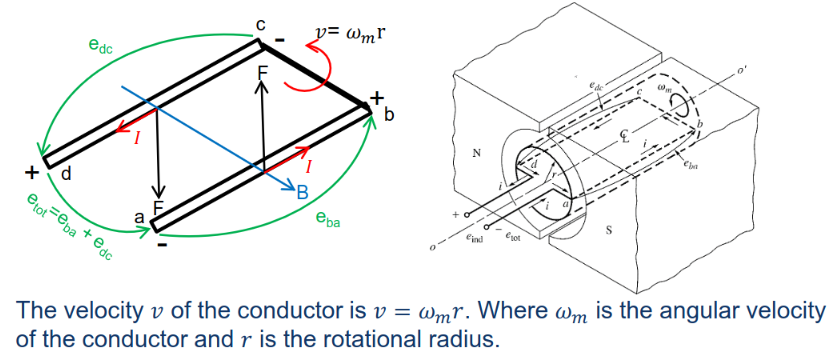
\includegraphics[width=0.5\linewidth]{Screenshots/single_loop}
	\caption{Single-loop Machine}
	\label{fig:singleloop}
\end{figure}

In each case (for each segment of conductor in the motor), we can analyze the force induced on the conductor, given by the Lorentz force law: $F = i \vec{l}\times \vec{B}$. It is straightforward to imagine, sections \textbf{bc, da}, that the magnetic field is parallel to the length of these segments, thus:
\begin{align*}
	\vec{F} &= i(\vec{l} \times \vec{B} ) = 0 \\ 
	\tau_{ind} &= \vec{r} \times \vec{F} = 0 \\ 
\end{align*}

And for the remaining two segments, where the force is given by:
\begin{align*}
	\vec{F} &= i\vec{l} \times \vec{B} = F_{tangent} \\
	\tau_{ab, cd} &= rilB \text{ (CCW)} \\
	\tau_{ind} &=
	\begin{cases}
		2rilB, \text{ } \frac{2}{\pi}\phi i & \text{ (Under pole faces)} \\
		0 & \text{ (Beyond pole faces)}	\end{cases}
\end{align*}

\subsection{The DC Machine}
There are a wide range of DC machines, each of which are generators that convert DC electric energy and motors that convert DC electric energy to mechanical energy. Some of the most common examples are enumerated below for further inquiry:
\begin{figure}[h]
	\centering
	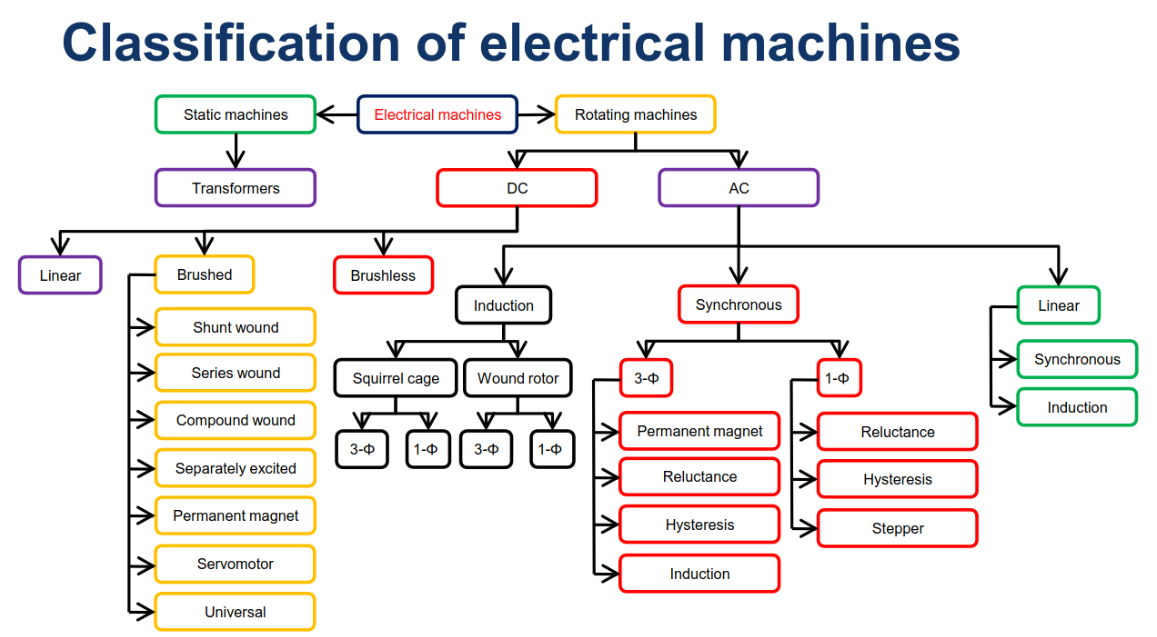
\includegraphics[width=0.4\linewidth]{Screenshots/classification_of_machine}
	\caption{Classifications of Some Electric Machines}
	\label{fig:classificationofmachine}
\end{figure}

The five major DC motors are:

\begin{itemize}
	\item The seperately excited DC motor.
	\item The shunt DC motor. 
	\item The permanent magnet DC motor.
	\item The series DC motor.
	\item The compound DC motor.	
\end{itemize}

Each of these motors can be approximated with an equivalent circuit:

\begin{figure}[h]
	\centering
	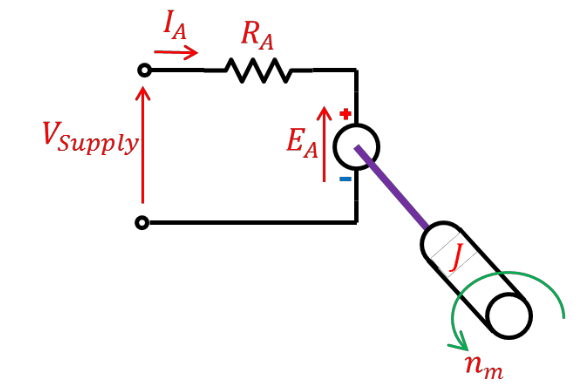
\includegraphics[width=0.5\linewidth]{Screenshots/equivalent_motor_circuit}
	\caption{Eqivalent Motor Circuit}
	\label{fig:equivalentmotorcircuit}
\end{figure}

Where the dynamics of the machine are dependent mainly on:

\begin{itemize}
	\item The $V_{supply}$ and maximum electrical ratings (amperage, voltage, thermal efficiency).
	\item Motor electrical and mechanical constants that dictate torque and induced voltage of the motor. Generally:
	\begin{align*}
		E_A &= \frac{ZP}{60a} \Phi n_m \text{ (Electrical Characteristics)} \\
		k'&= \frac{ZP}{60 a} \text{ (Electrical Constant)} \\
		\tau_{ind} &= \frac{ZP}{2\pi a} \Phi I_A \text{ (Mechanical Characteristics)} \\
		k &=  \frac{ZP}{2 \pi a} \text{ (Mechanical Constant)}
	\end{align*}
\end{itemize}

Where:
\begin{itemize}
	\item $Z = 2 C N_c$, where C is the coils and N is the number of turns per coil.
	\item $a = mP$, where m is the plex of the winding.
\end{itemize}
\subsection{Further Representation of The DC Machine}

I feel as though this textbook (Stephen Chapman) is shit, and it doesn't really demonstrate the DC machine properly, so I will consult another shit textbook (Stephen Umans) for further information on the DC machine.

\begin{figure}[h]
	\centering
	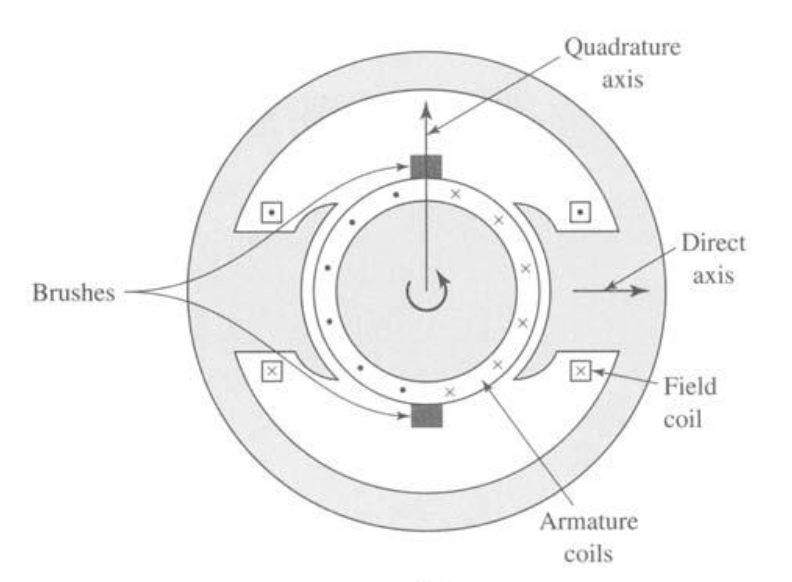
\includegraphics[width=0.5\linewidth]{Screenshots/DC_machine_schematic}
	\caption{DC Machine Schematic}
	\label{fig:dcmachineschematic}
\end{figure}

\subsection{Commutators}

The design of commutators (or brushes) in a rotating DC machine is of utmost importance. Commutators play a critical role in DC machine functionality, i.e providing a media for the as dynamic switches that connect windings of a rotor to the terminals of a DC machine just as the voltage in the loop switches polarity, in order to maintain an essentially constant dc output voltage. Some key aspects of commutator design are listed:

\begin{itemize}
	\item \textbf{Materials and Durability:} Commutators are typically made from hard-drawn copper segments insulated from eachother by a thin layer of micra. The choice of materials draws a balance between electrical and mechanical properties.
	\item \textbf{Segmentation and Insulation:} The segmentation of a commutator allows for the sequential current flow in the armature windings. The precision in and insulation of these segments directly impacts the efficiency of current reversal and overall operation of the DC machine.
	\item \textbf{Brush contact and Maintenance:} The design must also consider the necessity of continuous contact with the commutator segments. 
\end{itemize}

\textbf{Four loop, two pole DC Machine:}

\begin{figure}[h]
	\centering
	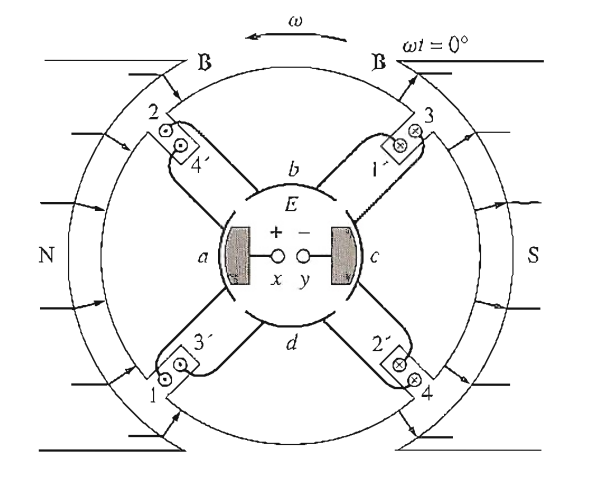
\includegraphics[width=0.3\linewidth]{Screenshots/four_loop_DC}
	\caption{Four Loop, two Pole DC Machine}
	\label{fig:fourloopdc}
\end{figure}

In order to develop an appreciation for commutation schemes, we shall analyze the four loop, two pole DC machine in figure \ref{fig:fourloopdc}. Each loop can be modelled as a wire with some inductance \textbf{to confirm}. The motor's $e_{ind}$ is found by:
\begin{align*}
	e_{ind} &= ( \vec{v} \times \vec{B}) \cdot l \\
	e_{ind} &= vbl
\end{align*}

This equation represents Faraday's law for the flux through the wire loops at some point of time ($v l = m^2 /s$). Thus we can represent the induced voltage as function of angular position. As seen in the graph: 
\begin{figure}[h]
	\centering
	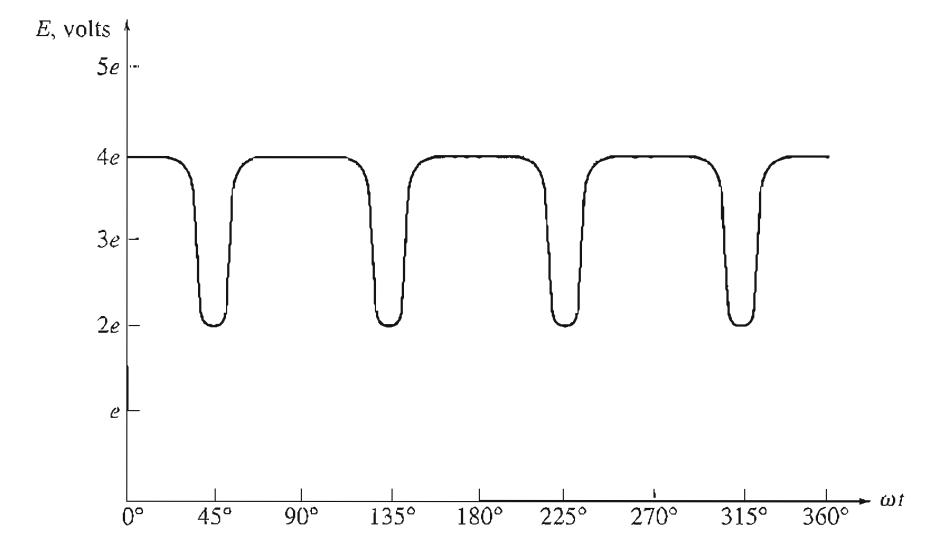
\includegraphics[width=0.4\linewidth]{Screenshots/four_loop_DC_voltage_theta}
	\caption{Four-loop $e_{ind}$}
	\label{fig:fourloopdcvoltagetheta}
\end{figure}

\subsection{Commutation and Armature Construction}

There are several ways in real DC machines in which the loops on the rotor (the armature) can be connected to its commutator segments. The method of connection becomes a function of:
\begin{itemize}
	\item Parallel current paths.
	\item Output voltage.
	\item The number and position of the brushes riding on the commutator segments. 
\end{itemize}

\textbf{The Rotor Coils:} Most rotor windings consist of diamond-shaped preformed coils which are inserted into the armature slots as a unit. The number of conductors on a machines aramature is generally given by:

\begin{align*}
	Z = 2CN_c
\end{align*}

Where: 
\begin{itemize}
	\item Z $=$ number of conductors on the rotor
	\item C $=$ number of coils on the rotor
	\item N$_C =$ number of turns per coil
\end{itemize}

We differentiate between \textit{mechanical} and \textit{electrical angle} to describe the positioning within the motor. The electrical angle describes the angle between a referenced magnetic pole, i.e: when one side of a coil, spanning $\pi$ radians is under the centre of a pole, the other side is under a pole of the opposite polarity. It is important to note that this is indepedent of the mechancical angle, which may be defined as the angle from some rotational axis. \textbf{confirm}. In a DC machine, we describe both angles with:
\begin{align*}
	\theta _e = \frac{P}{2}\theta_m
\end{align*}
Where $P$ is the number of poles on the machine.

Typical \textbf{commutator} construction is made up of copper bars insulated by a mica-type material. The copper bars are sufficiently thick to permit normal wear over the lifetime of the motor. The mica insulation is typically harder than the commutator material itself, so as the machine ages it is often necessary to undercut the commutator insulation to ensure that it doesn't stick up above the level of the copper bars. 


\begin{figure}[h]
	\centering
	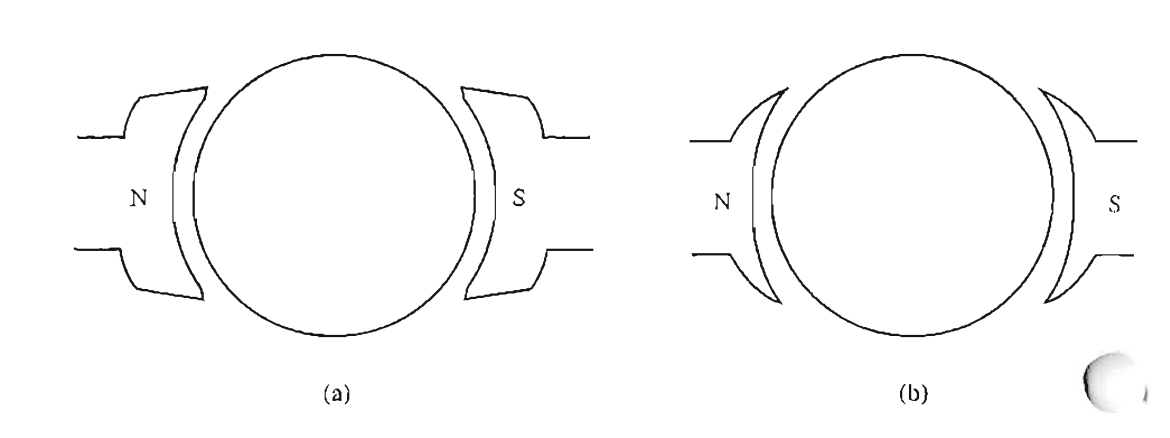
\includegraphics[width=0.4\linewidth]{Screenshots/pole_armature_geometry}
	\caption{Poles with extra air-gap width to reduce armature reaction. (a) chamfered poles; (b) eccentric or uniformly graded poles}
	\label{fig:polearmaturegeometry}
\end{figure}

\subsection{Winding Types:}

\textbf{Descriptive Parameters:} Before defining the winding types for DC machines, it helps to describe the winding types of the coils with displacements between conductors and so forth:
\begin{figure}[h]
	\centering
	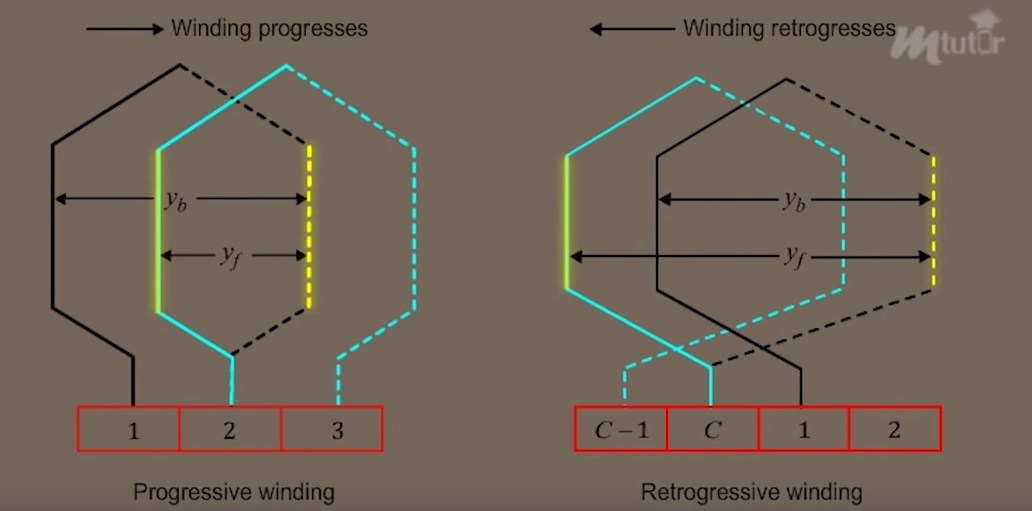
\includegraphics[width=0.4\linewidth]{Screenshots/pitch}
	\caption{Winding Pitch}
	\label{fig:pitch}
\end{figure}


\begin{itemize}
	\item \textbf{Pitch/Displacement:}
	\begin{itemize}
		\item \textbf{Back Pitch} ($y_b= $), Displacement between two conductors of a single coil.
		\item \textbf{Front Pitch} ($y_f=$), Displacement first conductor and second conductor of the next coil.
	\end{itemize}
\end{itemize}

\begin{itemize}
	\item \textbf{The Lap Winding:} The kap winding is typically used in high-current, low voltage applications.
	 \begin{figure}[h]
		\centering
		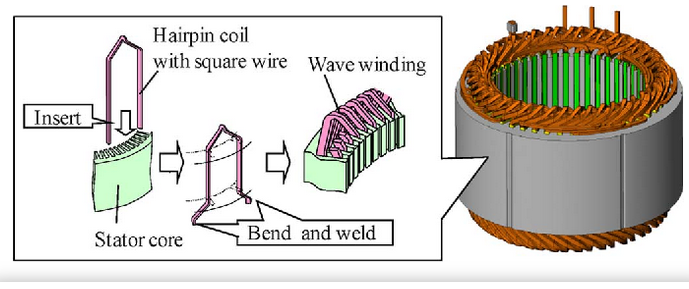
\includegraphics[width=0.4\linewidth]{Screenshots/lap_winding}
		\caption{Lap Winding}
		\label{fig:lapwinding}
	\end{figure}
	\begin{enumerate}
		\item Simplex Lap Windings, the terminating end of one coil is joined to the commutator segment and the starting end of the next coil is placed under the same pole. Also, the number of parallel 
		\item Duplex Lap Windings: The number of parallel paths between the pole is twice the number of poles. The duplex lap winding is mainly used for heavy current applications. Such a type of winding is obtained by placing the two similar winding on the same armature and connecting the commutator bars to one winding and the odd number to the second winding.
		\item Triplex Lap Windings: Windings are connected to one third of teh commuatator bars.
	\end{enumerate}
	\item \textbf{Current Paths:} As we shall see, the current paths in a winding are an important parameter. In lap windings, generally there are:
	\begin{align*}
		a= mP
	\end{align*}
	IN wave wound machines:
	\begin{align*}
		a = 2m
	\end{align*}
	\item \textbf{Retrogressive and Progressive:} as seen in figure \ref{fig:pitch}, we can see the difference between progressive and retrogressive windings. In progressive windings, each coil begins on $c_n$ and ends on $c_n+1$. In retrogressive windings, the coil beings on $c_n$ and ends on $c_n -1$.
	
	\item \textbf{The Wave Winding}
	\begin{enumerate}
		\item Simplex Wave Winding:
		paths is similar to the number of poles of the windings.
		\begin{align*}
			y_c &= \frac{2(C\pm 1)}{P} \\
			C&= \text{ number of coils on the rotor} \\
			P&= \text{ number of poles on the machine} \\ 
		\end{align*}
	\end{enumerate}
	\textbf{INCOMPLETE}
\end{itemize}

\subsection{Problems With Commutation in Real Machines:}

In theory, commutation processes are relatively straight forward, however, in reality, there are two major effects that occur in the real world to disturb it:
\begin{itemize}
	\item \textbf{Armature reaction:} When a load is connected to the DC machine, a current will flow in the armature windings. This in turn produces a magnetic field, which increases with a higher load. Armature reaction causes two major problems:
	\begin{enumerate}
		\item \textbf{Neutral Plane Shift:}
		\begin{figure}[h]
			\centering
			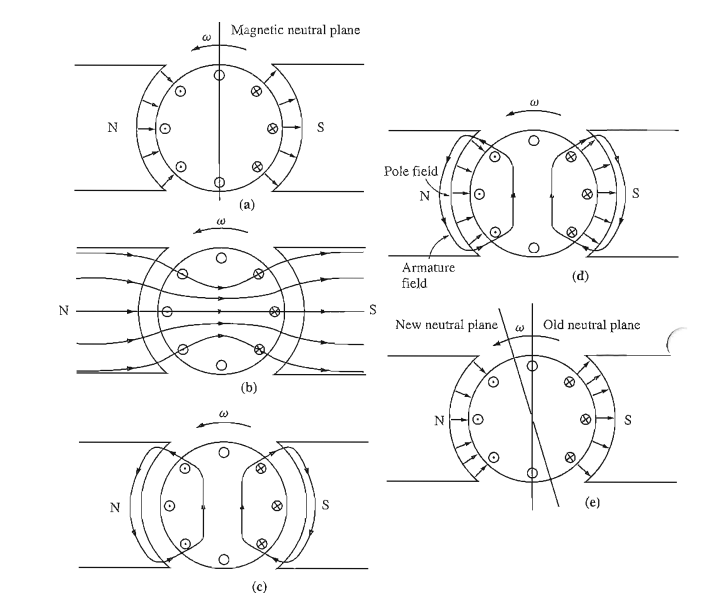
\includegraphics[width=0.4\linewidth]{Screenshots/neutral_plane_shift}
			\caption{Neutral Plane Shift}
			\label{fig:neutralplaneshift}
		\end{figure}
		The effect of neutral plane shift can be generalized as the overall flux in the air gap is skewed and non-uniform. Generally, the neutral plane will shift in the direction of motion for a generator and opposite to the direction of motion for a motor. This also effects the functioning of the commutator, if the plane is set such that there is a zero voltage shorting the commutator, when the plane is shifted there is a non-zero voltage across the commutator, which can result in sparking at the brushes.
		\item \textbf{Flux weakening:} In order to understand flux weakening, we must consider a magnetization curve. Most DC motors operate at saturation points. Thus, when mmf increases or decreases as a result of armature reaction. In generators, it simply reduces the voltage for any given load, however for motors, when the flux is decreased, its speed increases. It is possible for some shunt DC motors to reach a runaway condition where the speed of the motor just keeps increasing until the machine is disconnected from the power line or destroys itself.
		\begin{figure}[h]
			\centering
			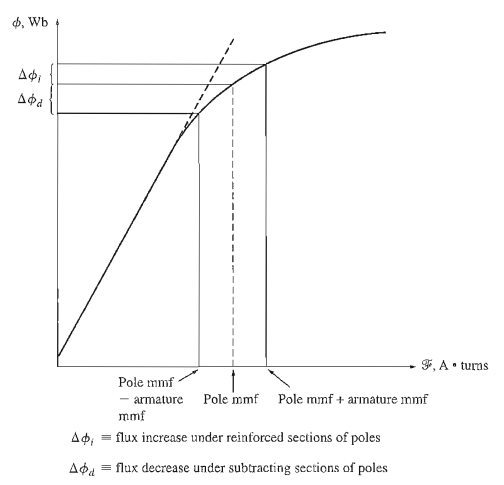
\includegraphics[width=0.3\linewidth]{Screenshots/flux_weakening}
			\caption{Flux Weakening}
			\label{fig:fluxweakening}
		\end{figure}
		
	\end{enumerate}
	\item \textbf{$L di/dt$ voltages} or \textbf{inductive kick}: We know the voltage equation: $v = L \frac{di}{dt}$ for inductance. We also know that there is a brief short in commutator brushes at certain points of operation. Thus, the short-circuit current changes polarity rapidly. If a machine is turning at $800$ r/min, and there are $50$ commutator segments, the commutator will move under the brush and clear it in $0.0015$s. Therefore, the rate of change in current with respect to time in the shorted loop must average $di/dt = \frac{400A}{0.0015s} = 266,667$A/s. Clearly, if there is even a tiny inductance in the loop, a significant voltage kick will result from this process, resulting in the same arcing as in the plane shift process.
\end{itemize}

Solutions to the problems:
\begin{itemize}
	\item Brush shifting
	\item Commutating pole or interpoles
	\item Compensating windings
\end{itemize}

As we have seen previously, magnetization curves are generally non-linear unless they are operated around the knee point (before the saturation point). Thus, when armature reaction is present it makes it difficult to model and work with DC machines. If a machine has armature reaction, its flux will be reduced with each increase in load. The total magnetomotive force in a shunt DC motor is the field circuit magnetomotive force less the magnetomotive force due to armature reaction:
\begin{align*}
	\mathsf{F}_{net} = N_F I_F - \mathsf{F}_{AR}
\end{align*}



\subsection{Generated Voltage and Induced Torque Equations of DC Machines}

The induced voltage in any machine is dependent upon three factors:
\begin{itemize}
	\item The flux $\Phi_B$ in the machine
	\item The speed $\omega_m$ of the machines rotor
	\item A constant that is dependent on the construction of the machine
\end{itemize}

The voltage out of the armature of a real machine is thus:
\begin{align*}
	E_A = \frac{ZvBl}{a}
\end{align*}
If there are $P$ poles on the machine, then the portion of the area associated with each pole is the total area $A$ divided by the number of poles $P$:
\begin{align*}
	A_P = \frac{A}{P} = \frac{2\pi r l B}{P} 
\end{align*}
The total flux per pole is then:
\begin{align*}
	\Phi_B = B \frac{2 \pi r l B}{P} 
\end{align*}
Expressing this as the rate of change of flux in the machine is thus:
\begin{align*}
	E_A &= \frac{Z r \omega_m Bl}{a} \\
	&= \frac{ZP}{2 \pi a} \frac{2\pi r l B}{P} \omega_m \\
	&= K \Phi_B \omega_m  \textbf{ (general form, $\omega_0$)}\\
	&= K' \Phi_B n \text{ (RPM form)} \\
	\text{where}& \\
	K &= \frac{ZP}{2\pi a} \text{ (Rad/s)} \\
	K' &=  \frac{ZP}{60 a} \text{ (Rev/m)} 
\end{align*}

Recall: $Z = 2C N_c$ which is the number of conductors in a machine, given by coils times  current path number, $P =$ the number of poles in a machine. In most cases, we measure angular velocity of the machines rotor in revolutions per minute. A formula for this conversion is given by:
\begin{align*}
	\omega_m = \frac{2\pi}{60}n_m
\end{align*}

And the torque relation for a DC machine is given by:

\begin{align*}
	\tau_{ind} &= \frac{ZP}{2 \pi a} \phi I_A \\
\end{align*}

\subsection{Power Flow and Losses}

The efficiency of the DC machine is given by the transfer function ratio:
\begin{align*}
	\nu = \frac{P_{out}}{P_{in}}\times 100 
\end{align*}
We categorise losses as such:

\begin{itemize}
	\item Electrical or copper losses $I^2R$ 
	\item Brush losses
	\item Core losses
	\item Mechanical losses
	\item Stray load losses
\end{itemize}

\begin{figure}[h]
	\centering
	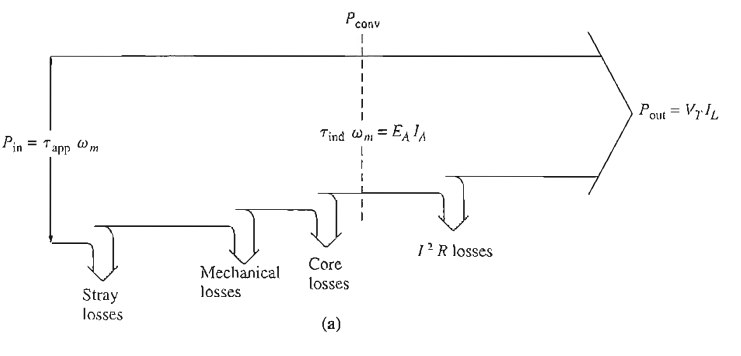
\includegraphics[width=0.4\linewidth]{Screenshots/power_diagram}
	\caption{Loss Diagram}
	\label{fig:powerdiagram}
\end{figure}

\subsection{Separately Excited and Shunt DC Motor}

The equivalent circuit of a shunt DC motor describes a motor whose field is powered directly from a DC terminal. We can also describe a seperately excited motor (a motor whose field is supplied from a seperate supply) when the supply voltage is assumed constant with the same circuit as the operation is practically the same.

\begin{figure}[h]
	\centering
	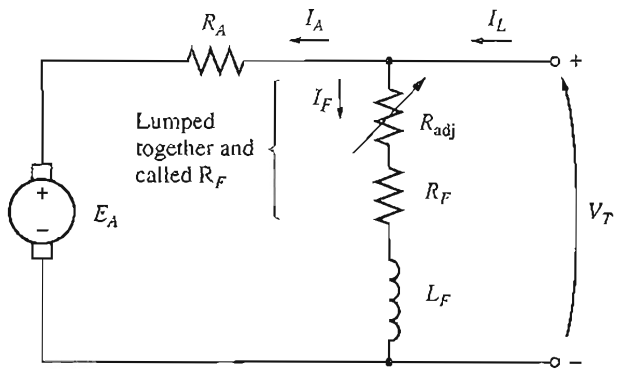
\includegraphics[width=0.5\linewidth]{Screenshots/equivalent_motor_circuit1}
	\caption{Shunt DC Schematic}
	\label{fig:equivalentmotorcircuit1}
\end{figure}

How does a shunt DC motor respond to a load?
\begin{itemize}
	\item \textbf{When the load increases:}  The load torque $\tau_{load}$ will exceed $\tau_{ind}$ in the machine, and the motor will start to slow down. 
	\item \textbf{When the motor slows down:} Its internal generated voltage drops, so the armature current in the motor $I_A =(V_T - E_A)/R_A$ increases. 
	\item \textbf{As the armature current rises:} The induced torque $\tau_{ind} = K \phi I_A$ in the motor increases. 
	\item And finally the induced torque will equal the load torque at a lower mechanical speed of rotation.
\end{itemize}

The output characterisitic of a shunt DC motor can be derived from the induced voltage and torque equations plus KVL:

\begin{align*}
	V_T &= E_A + I_A R_A \\
	V_T &= K \phi \omega_m + I_A R_A \\
	I_a &= \frac{\tau_{ind}}{K\phi} \\
\end{align*}
Combining these equations yields:
\begin{align*}
	V_T &= K \phi \omega_m + \frac{\tau_{ind}}{K \phi} R_A
\end{align*}

Finally, solving for the motor's speed yields:

\begin{align*}
	\omega_m = \frac{V_T}{K \phi} - \frac{R_A}{(K\phi)^2}\tau_{ind}
\end{align*}

In case of an initial approximation of the shunt DC motor, if we assume constant flux, no armature reactions, and motor speed/current are known, then it is possible to evaluate speed at any other value of the load. To do this:

\begin{itemize}
	\item Use KVL to evaluate the current distribution across the circuit. 
	\item Use calculate currents to evaluate voltage across the armature. 
	\item Evaluate speed. As flux is constant, we can use the ratios of $E_A$ at no load and any other computed point to evaluate the speed. 
	\item We can then also evaluate torque and other motor parameters.
\end{itemize}

However, the flux is generally dynamic and can be controlled by varying the field current. The effects of magnetizing are non-linear and typically need to reference some sort of magnetizing curve in order to determine circuit parameters, as they cannot be determined analytically.


\subsection{PMDC Motor}

PMDC Motors have some benefits when comparing to shunt DC motors:
\begin{itemize}
	\item Smaller, more cost effective.
	\item Do not require an external field circuit.
\end{itemize}

However some cons can be listed too: \textbf{THIS IS CLEARLY UNFINISHED}

\begin{itemize}
	\item Lower induced torque per ampere of armature current than a shunt motor of the same size and construction.
\end{itemize}

\newpage

\textbf{Magnetization Curve of the PMDC motor}

We know:

\begin{align*}
	E_A &= K_e \Phi n_m \\
\end{align*}

If $n_m = $ constant, then $E_a$ varies with $\Phi$. This relation can be used to derive an approximation for the magnetization curve of the permanent magnets of a PMDC motor. Starting with:

\begin{align*}
	\vec{B} = \mu H
\end{align*}
Where, $\vec{B}$ is the magnetic field, $\mu$ is the magnetic permeability of the material, and $H$ is the magnetic intensity.

We can find magnetic intensity as a function of magnetomotive force for a winding with $N$ turns:

\begin{align*}
	\mathsf{F} = NI = H d
\end{align*}

Where $N$ and $d$ are constants (turns, average path length) in context of the PMDC motor, thus:
\begin{align*}
	I_a \propto H
\end{align*}
Therefore we can theoretically, or experimentally approximate the permeability of the magnetic circuit, and  plot its magnetization curve with:

\begin{align*}
	\vec{B} &= \mu H \\
	\mathsf{F} &= NI = Hd \\
	E_a &= K_e \Phi n_m
\end{align*}

We can assume $K_e$ and $n_m$ constant, and $E_a$ is induced voltage in the armature. Thus, with some algebra:

\begin{align*}
	E_a &= k_e \vec{B} A n_m \\
	 &= k_e \mu H A n_m \\
	&=  k_e \mu N I_a A n_m \\
	\text{Assuming $n_m$, $A$, $N$}&\text{ $k_e$ approximately constant} \\
	\frac{\delta{E_a}}{\delta t} &\approx \mu \frac{\delta I_a}{\delta{t}} \\
\end{align*}



\section{Week 4: Transformers}

One of the most prevalent applications of mutual inductance is the ability to \textit{step-up} and \textit{step-down} voltages. In the late $19^{th}$, when power generation and transmission was a feasible idea, power stations used to be required to be in close proximity to the consumers, otherwise losses from $I^2R$ heating were far too great. This changed with the ability to manipulate voltage levels via transformers at geographical points, for high-voltage transmission that is still implemented today. Transformers also find a wide variety of application in low-power, low-current electronic and control circuits for performing impedance matching, isolation etc. \newline

But how do tranmission losses decrease at higher voltages? To understand this, it is important to consider most important relations in transformer modelling. They are written for convenience:

\begin{align*}
	\frac{V_p}{V_s} &= \frac{I_s}{I_p} =  \frac{N_p}{N_s} = a \\
	\frac{N_p}{N_s}^2 Z_s &= Zs' \textit{ ("Referred impedance")}
\end{align*}

Where referred impedance is the impedance on the secondary 'seen' from the input terminals (primary side). We know that AC power is given by:

\begin{align*}
	P_{rms} = \frac{1}{\sqrt{2}} V I  = \frac{V^2}{\sqrt{2} Z } =\frac{V^2 Z}{\sqrt{2}}  
\end{align*}

Using our model, for a step up transformer, the windings on the primary are less than the windings on the secondary ($N_p < N_s$). Thus, 
\begin{align*}
	V_s &= \frac{N_s}{N_p} V_p \\
	I_s &= \frac{N_p}{N_s} I_p
\end{align*}

But most importantly, the relation that encapsulates both of these values:
\begin{align*}
	Z_s' = \frac{N_p}{N_s}^2 Z_s
\end{align*}

Now, considering just a regular transmission line, the power lost for an impedance $Z$, given by its a lumped parameter model with parasitic capacitance and inductance, with current $I$ is modelled by the spice schematic:

\begin{figure}[h]
	\centering
	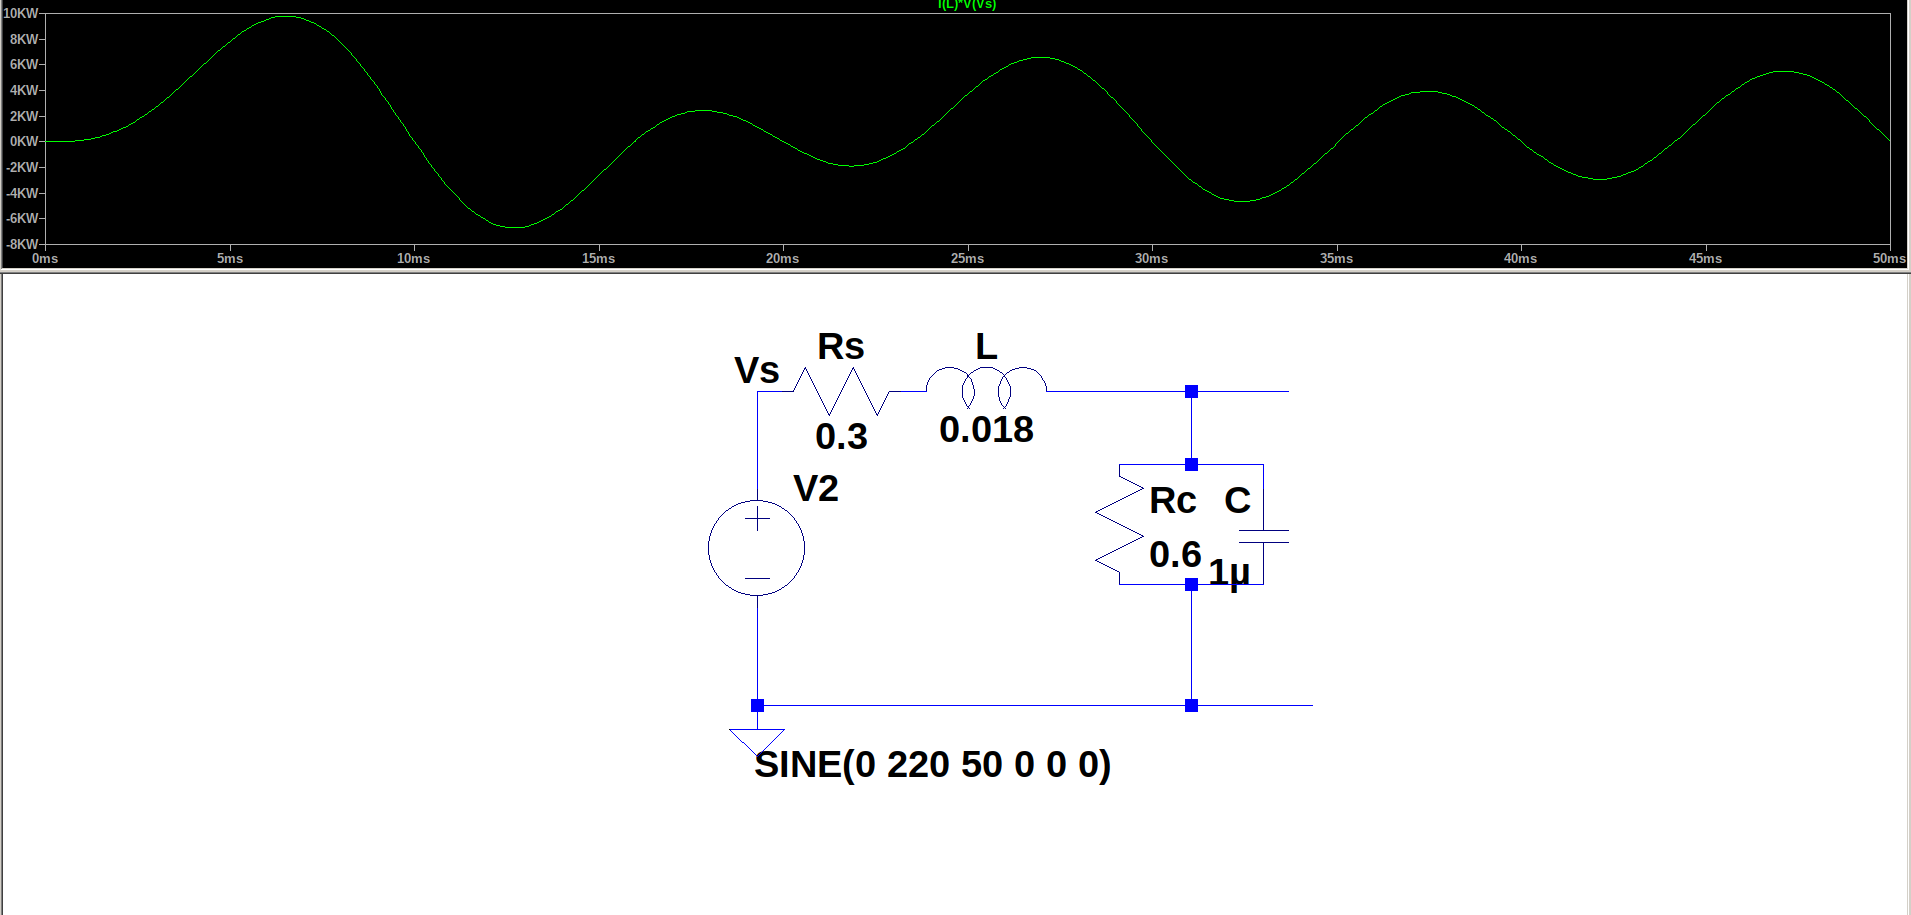
\includegraphics[width=0.5\linewidth]{Screenshots/transmission_line_power}
	\caption{Lumped Parameter Model of Transmission Line}
	\label{fig:transmissionlinepower}
\end{figure}


\begin{figure}[h]
	\centering
	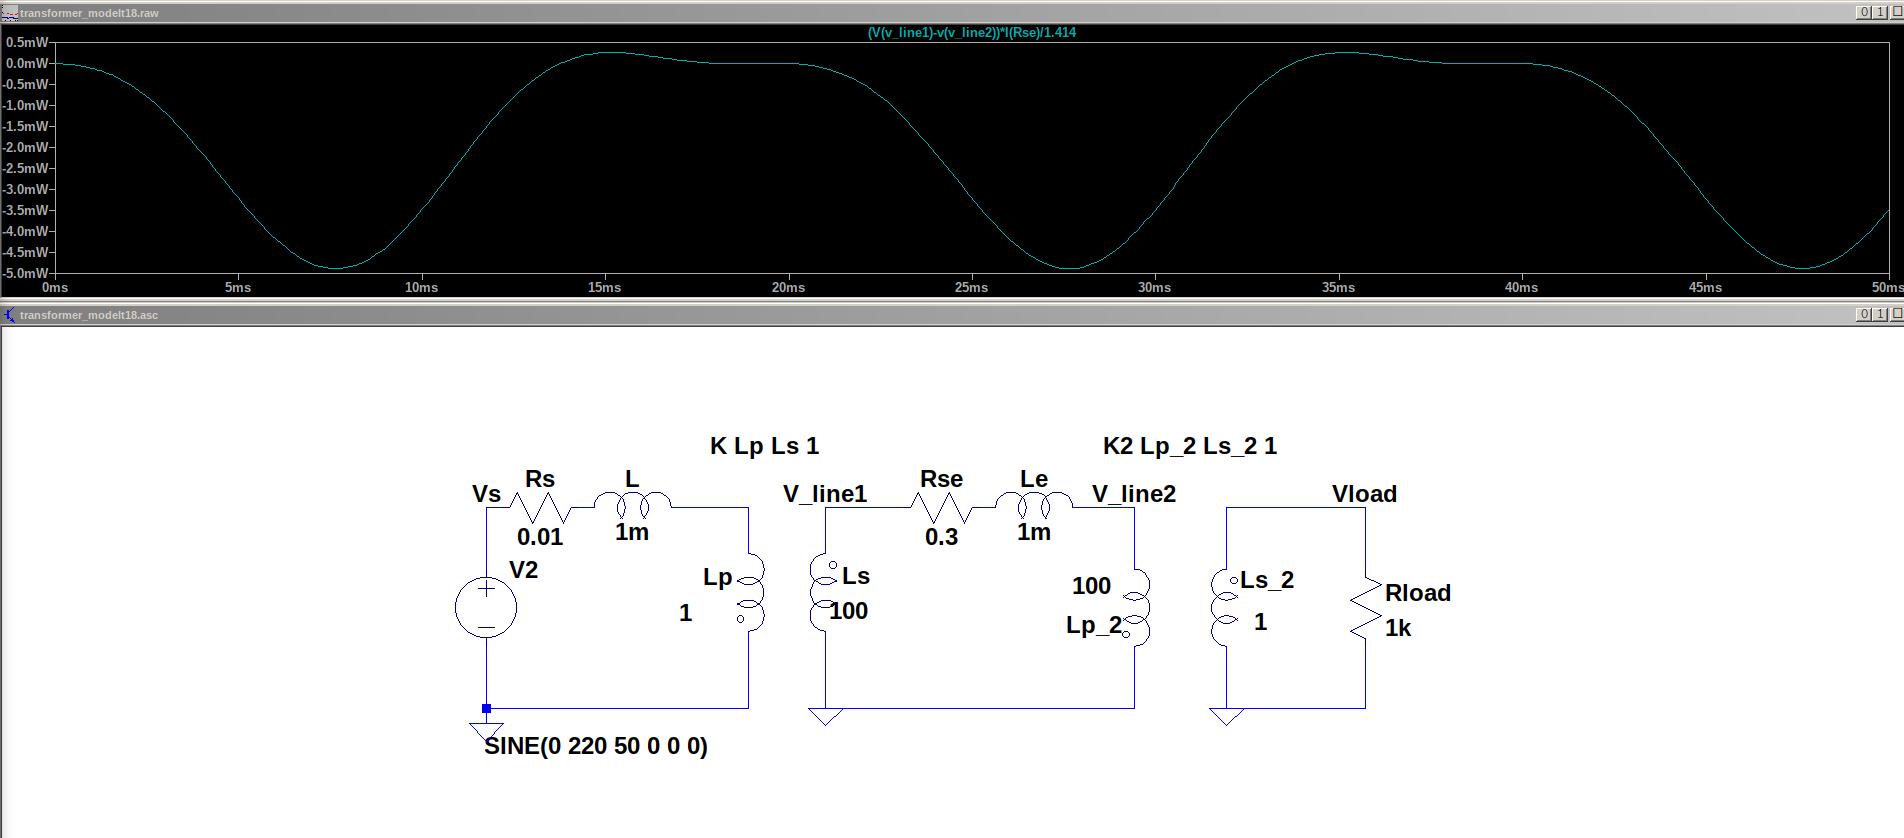
\includegraphics[width=0.4\linewidth]{Screenshots/transmission_line_power1}
	\caption{Transmission Schematic}
	\label{fig:transmissionlinepower1}
\end{figure}

And notice the magnitude difference of power loss in figure \ref{fig:transmissionlinepower1}, a factor of $10^6$ difference, although this may not be completely accurate, it is a demonstration of its utility.

\subsection{Mutual Inductance:}

Very often, one will find, either accidentally or by design that magnetic flux through a circuit will vary with time because of varying currents in a nearby circuit. This gives rise to an induced emf. This process is called mutual induction. 

If we imagine two closely spaced coils, one with current $I_1$ flowing in it, we know that the resultant magnetic field is given by:
\begin{align*}
	\mu_0 n I = \vec{B}
\end{align*}
\begin{figure}[h]
	\centering
	\includegraphics[width=0.4\linewidth]{../../PVB301/Notes/Screenshots/mutual_inductance}
	\caption{Mutual Inductance}
	\label{fig:mutualinductance}
\end{figure}

But, we also know Faradays law says that a changing magnetic flux induces a voltage, or emf, given by. So what happens if the second coil, with no flux, is close enough in proximity to the coil with the current through it? This is the most common illustration of our subject, \textbf{mutual inductance}, which is described by:

\begin{align*}
	M_{21} &\equiv \frac{N_2 \Phi_{21}}{I_1} \\
	\Phi_{21} &= \frac{M_{21}}{N_2}I_1
\end{align*}

Clearly, our mutual inductance is a function of the geometry and turns of our coils. With varying current with time, we see that:

\begin{align*}
	\varepsilon = -N_2 \frac{d \Phi_{21}}{dt} = -M_{21} \frac{dI_1}{dt}
\end{align*}


\subsection{Construction}

Transformers are generally constructed with laminated cores, to reduces losses associated with eddy currents. Two commonly used configurations are shown below:
\begin{figure}[h]
	\centering
	\includegraphics[width=0.4\linewidth]{../../PVB301/Notes/Screenshots/transformers}
	\caption{Transformer Schematics: a) core type b) shell type}
	\label{fig:transformers}
\end{figure}

These transformers are used in applications where the AC signal is no greater than a few hundred hertz. These are usually \textbf{silicon steel} transformers, with laminations being roughly $3$cm in width. The cores of small transformers used in communication circuits at high frequencies
and low energy levels are sometimes made of compressed powdered ferromagnetic alloys known as ferrites.

\subsection{No-load conditions}

The schematic below shows the typical representation of transformer circuit schematics, however the windings are actually interleaved in practice.

\begin{figure}[h]
	\centering
	\includegraphics[width=0.4\linewidth]{../../PVB301/Notes/Screenshots/transformers_no_load}
	\caption{Transformer with open secondary.}
	\label{fig:transformersnoload}
\end{figure}

A small steady-state current flowing in the primary establishes an alternating flux in the magnetic circuit. This flux induces an emf in the primary equal to:

\begin{align*}
	e_1 = \frac{d\lambda_1}{dt} = N_1 \frac{d \phi }{dt}
\end{align*}

Where:

\begin{itemize}
	\item $\lambda_1$ is the flux linkage in the primary windings.
	\item $\phi$ is the flux in the core linking both the windings.
	\item $N_1$ is the number of turns in the primary winding.
\end{itemize}

In typical transformers there is an extra term for leakage flux, this flux is a small percentage of the core flux, and is quite justifiable to neglect it for the time being. Under the condition that the instantaneous flux is a sinusoid, the induced voltage is typically represented in the manner: $\psi = \phi_{max} sin(\omega t)$

\subsection{Loaded Conditions}

When a transformer is loaded, its behaviour is defined by the functions:

\begin{align*}
	V_1 &= -N_1 \frac{d\Omega_m}{dt} \\
	V_2 &= -N_2 \frac{d\Omega_m}{dt} \\
	\frac{V_2}{V_1} &= \frac{N_2}{N_1} 
\end{align*}

Clearly, the conditions hold:

\begin{itemize}
	\item When $N_1 <N_2$, we have a step-up transformer.
	\item When $N_1 > N_2$, we have a step-down transformer.
\end{itemize}

In the ideal transformer, with a resistive load, why neglect energy losses in transformer windings and core, thus the statement: $I_1 V_1 = I_2 V_2$ can be used for quick approximations. Furthermore, the value of load resistance determines the value of secondary current, since $I_2 = V_2 /R$. The current in the primary is $V_1/R_{eq}$, where $R_{eq}$ is viewed from the primary side, given by:

\begin{align*}
	\text{recall } n &= \frac{N_p}{N_s} = \frac{V_p}{V_s} = \frac{I_s}{I_p}\\
	Z_s &=  \frac{I_p Z_p}{n} \\
	Z_p &= \frac{I_s Z_s n}{I_p} \text{, and } \frac{I_s}{I_p} = n \\
	Z_{load(p)} = (\frac{N_1}{N_2})^2 Z_{load(s)}
\end{align*}
\begin{figure}[h]
	\centering
	\includegraphics[width=0.4\linewidth]{../../PVB301/Notes/Screenshots/transformers_load1}
	\caption{Loaded Transformer}
	\label{fig:transformersload1}
\end{figure}

\subsection{Realistic Transformer Models}

\begin{figure}
	\centering
	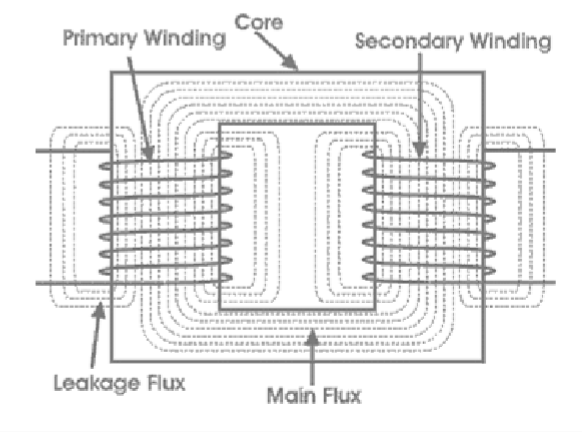
\includegraphics[width=0.4\linewidth]{Screenshots/real_transformer}
	\caption{Real Transformer Losses}
	\label{fig:realtransformer}
\end{figure}

In order to develop realtistic transformer models, we either take a physical reasoning or mathematical reasoning approach based upon the classical theory of magnetically coupled circuits.

\begin{figure}[h]
	\centering
	\includegraphics[width=0.4\linewidth]{../../EGB240/Notes/Screenshots/realistic_transformer1}
	\caption{Development of Realistic Transformer Model}
	\label{fig:realistictransformer1}
\end{figure}

In figure \ref{fig:realistictransformer}, we see a circuit model that more accurately represents the behaviour of a realistic transformer. 

\begin{itemize}
	\item There is no perfect coupling between windings (leakage inductance).
	\item A current is required to establish the magnetic field (magnetizing inductance).
	\item There are losses in the transformer windings. These losses are represented by small resistances due to the copper windings. 
	\begin{align*}
		P_{lost} &= I^2 R \\
		R &= \frac{d}{\sigma A} = \rho \frac{d}{A} 
	\end{align*}
	\item There are losses in the core. The core losses, which are a result of hysteresis losses and eddy current losses, can be minimized by a laminated core. Lamination of the core results in higher resistance segments and a larger number of current pathways.
\end{itemize}

Essentially, we can greatly simplify calculations for transformer circuits by \textit{ignoring} the shunt branch in our model, as core losses are essentially much lower in modern laminated steel-core transformers than that of the windings in the circuit. With our newly formed model, we can derive a number of useful relations/design techniques.

\begin{itemize}
	\item \textbf{Primary or HV Side Model:} By looking into the terminals from the perspective of the voltage source, we can solve for useful circuit parameters $V_p$ and $I_p$ that essentially describe the entire circuit. The only extra step (ignoring core/hysterisis losses), is \textbf{referring} the load impedance to the primary side. The referred impedance is simply a function of the turns ratio. An instructive excercise would be \textbf{deriving this model}
	\begin{align*}
		Z_{load}' = (\frac{N_p}{N_s})^2 Z_{load} 
	\end{align*}
	\item \textbf{Secondary Side Model:} By simply inverting the primary side model, we can arrive at the secondary side model.
\end{itemize}

The equivalent circuits have the additional advantage of the ability to determine the total equivalent impedance $Z_{eq}= R_{eq} + X_{eq}$ via a \textbf{short circuit test}. On the other hand, the determination of distinct leakage reactances $X_{l1}$ and $X_{l2}$ is a bit more difficult. In fact, without knowledge of the turns ratio (based upon knowledege of the internal structure of the transformer), it is impossible to construct specific values for the leakage reactances.

\subsection{Magnetizing Current of Transformer}

We can derive an expression for magnetizing current that is particularly instructive for our model of the transformer. First, imagine a voltage source, connected in series with a resistance and with $N_p$  windings around a leg of a transformer. On the opposite side, there is another leg with $N_s$ windings that is driving a load. We know we can model the transformer with a magnetic circuit. The equations are thus:

\begin{align*}
	\sum MMF &= \mathsf{F}_{sources} - \mathsf{F}_{sinks} = 0 \\
	I_P N_P &= \Phi \mathsf{R} + I_s N_s \\
	\Phi &= \frac{I_p N_p - I_s N_s}{\mathsf{R}_{core}} \\
	V_p &= N_P \frac{d}{dt} (\frac{I_p N_p - I_s N_s}{\mathsf{R}_{core}}) \\
	V_p &= \frac{N_p^2}{\mathsf{R}_{core}} \frac{d}{dt} (I_p - I_s N_s/N_p) \\
	\text{from } L&= \frac{N^2}{\mathsf{R}_{total}} \\
	V_p &= L_m \frac{d}{dt} (I_p - I_s N_s / N_p) \\
	\text{But we know }V&= L\frac{dI}{dt} \\
	V_p &= L_m \frac{dI_m}{dt} \\
\end{align*}

Where $L_m$ is the magnetizing inductance, and is typically very large.

\textbf{To explore further:}
\begin{itemize}
	\item The primary current must not only magnetize the core, it must also supply current to the load connected to the secondary.
	\item $I\phi$: The \textit{exciting component} is defined as the additional primary current required to produce the resultant magnetic flux. It can be resolved a core-loss component $I_c$ to be in phase with the emf $E_1$ and a magnetizing component $I_m$ lagging $E_1$ by $\pi/2$
\end{itemize}


\subsection{Open and Short Circuit Parameter testing:}

\textbf{Short Circuit Test:} The short circuit test can be used to find the equivalent series impedance; $R_{eq} + j X_{eq}$. For convenience, the high-voltage side, particularly in this textbook (Fitzgerald), is taken as the primary. Typically, the series impedance of a transformer is relatively small, typically an applied primary voltage on the order of 10 to 15 percent or less of the rated value will result in the rated current.

\textbf{Open Circuit Test:} The open-circuit test is performed with the secondary open-circuited and rated voltage impressed on the primary. Under this condition an exciting current of a few percent of full-load current is obtained. Rated voltage is chosen to insure that the magnetizing reactance will be operating at a flux level close to that which exists under normal operating conditions.

\subsection{Voltage Regulation:}

Voltage regulation of a transformer is defined as the change in secondary terminal voltage from no load to full load and is usually expressed as a percentage of full-load value. This is a figure of merit in transformers, in which a low value indicates that load variations on the secondary of the transformer will not significantly effect the magntitude of voltage being applied to the load.

\subsection{Autotransformers:}

Auto transformers are a different topology of transformer. Unlike the two-winding transformer, the windings on the $ab$ section of the autotransformer, as shown in figure \ref{fig:autotransformers}, is common to both the primary \textit{and} secondary circuits. The winding $ab$ must be provided with extra insulation to ensure it is insulated against the full maximum voltage of the autotransformer. 
\begin{figure}[h]
	\centering
	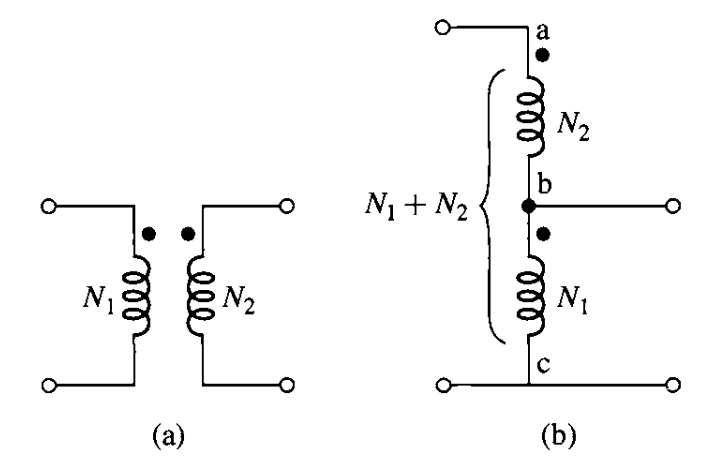
\includegraphics[width=0.3\linewidth]{Screenshots/auto_transformers}
	\caption{Auto transformer}
	\label{fig:autotransformers}
\end{figure}

\begin{itemize}
	\item \textbf{Questions:} Why does an actually meant by the statement: The higher rating as an autotransformer is a consequence of the fact that not all the 550 kVA has to be transformed by electromagnetic induction. In fact, all that thetransformer has to do is to boost a current of 208 A through a potential rise of 240 V,	corresponding to a power transformation capacity of 50 kVA. From the textbook example?
\end{itemize}


\section{Week 5: Three Phase Circuits:}

The majority of AC power generation, transmission and distribution utilize three-phase circuits in order to transmit electric power. In order to consider the method of generation of three-phase power sources, imagine a \textit{elementary two-pole, three-phase generator}
\begin{figure}[h]
	\centering
	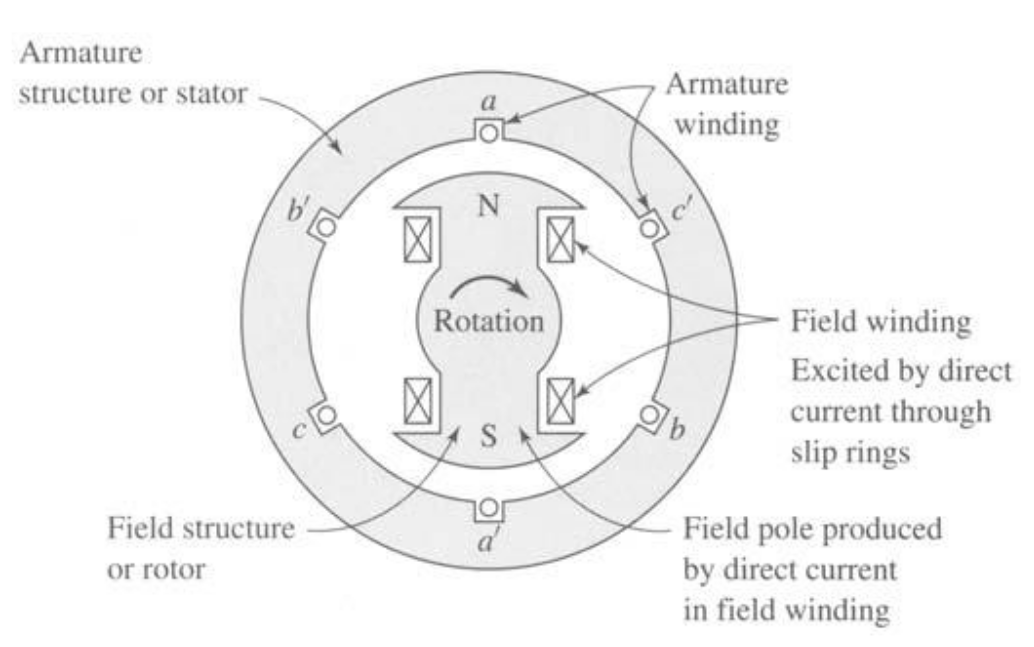
\includegraphics[width=0.4\linewidth]{Screenshots/screenshot001}
	\caption{Two-Pole, Three-Phase generator}
	\label{fig:screenshot001}
\end{figure}

As we can see, the armature windings are displaced $120$ electrical degrees in time as a result of the phases being displaced $120$ degrees in space. Generally, the time origin and reference axis are chosen on the basis of analytical convenience. The three phases of the winding can be connected in two possible ways, as shown in figure [\ref{fig:wyedelta2}]
\begin{figure}[h]
	\centering
	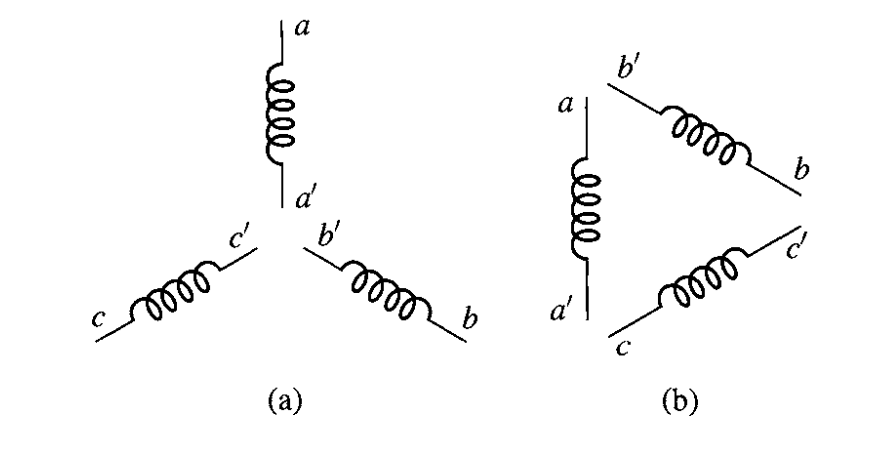
\includegraphics[width=0.4\linewidth]{Screenshots/wye_delta_2}
	\caption{Wye Delta Windings}
	\label{fig:wyedelta2}
\end{figure}

As such, these windings combinations result in a balanced three-phase system. Unbalanced systems can occur due to voltages begin unbalanced in magnitude or phase, or the impedances may not be equal.
\subsection{Balanced State Operation:} In balanced state operation of a three-phase AC circuit, there are three active wires (or high voltages) that are are out of phase by $\angle120$ . In such a case, the load in on each net must also be balanced, otherwise there is return current, which must be returned through neutral.


\begin{itemize}
	\item AC systems typically operate in balanced state.
	\item Three phase AC motors are self starting and do not require special starting or running circuitry, whereas single AC systems require capacitors to start.
\end{itemize}

\begin{figure}[h]
	\centering
	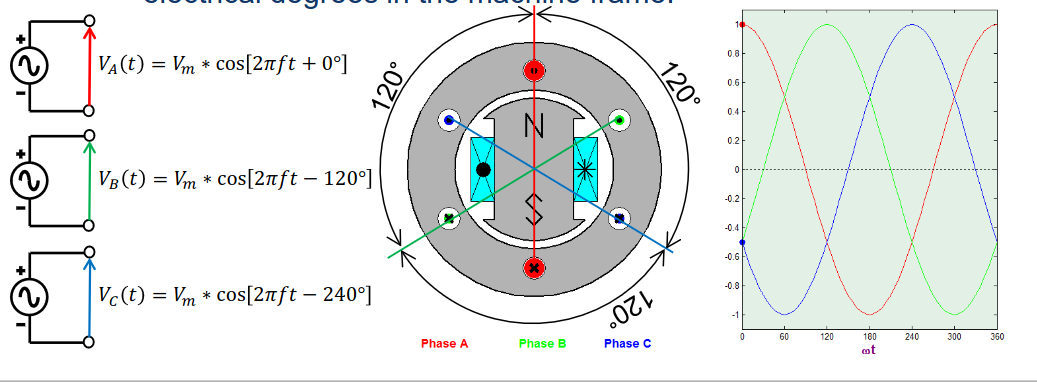
\includegraphics[width=0.4\linewidth]{Screenshots/real_cap_model}
	\caption{Three Phase AC Motor}
	\label{fig:three_phase}
\end{figure}

The three phases in figure [\ref{fig:three_phase}] represent seperate AC generators. The electrical angle between each must differ by and equal $2.1$ radians. These three phases are referred to as:

\begin{enumerate}
	\item A Phase
	\item B Phase
	\item C Phase
\end{enumerate}

There are only a two possibilities of this combination, 
\begin{figure}[h]
	\centering
	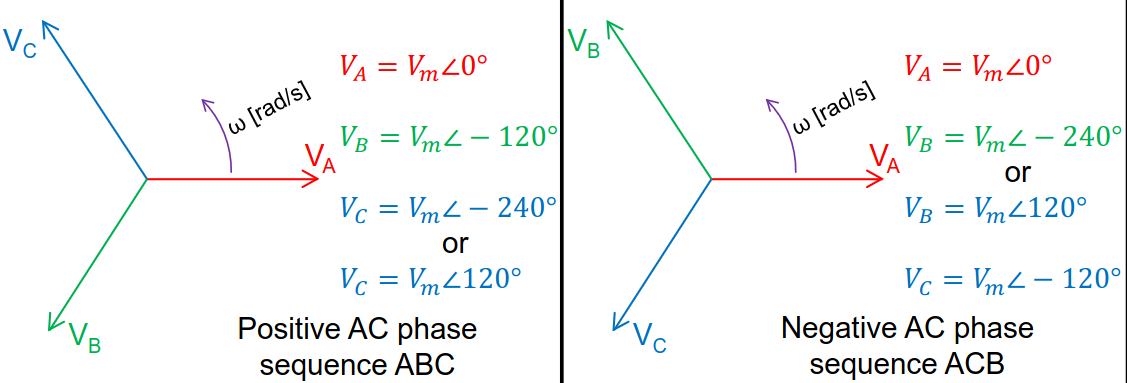
\includegraphics[width=0.4\linewidth]{Screenshots/balance_3phase}
	\caption{Balanced Three-Phase AC Voltage Sources}
	\label{fig:balance3phase}
\end{figure}

With a little further investigation, one can see that the sum of the phasor voltages is zero. 

\subsection{Wye and Delta}

Regardless of the generation of the voltage, there are only two methods of connecting a three phase system, (which some electricians are very familar with).

\begin{figure}[h]
	\centering
	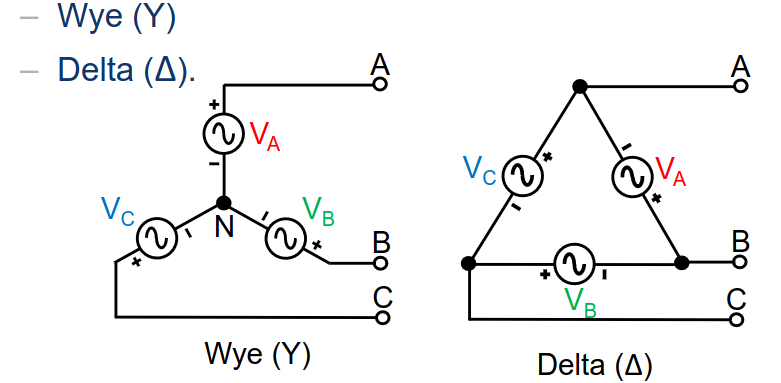
\includegraphics[width=0.4\linewidth]{Screenshots/wye_delta}
	\caption{Wye Delta Connections}
	\label{fig:wyedelta}
\end{figure}

But first we will establish some terminology:

\begin{itemize}
	\item \textbf{Line Voltage:} Refers to the AC voltage accross any pair of lines. 
	\begin{align*}
		\text{Wye (Y):} &= |V_{AB}|= \sqrt{3} |V_{AN}| =\sqrt{3} |V_A| \\
		\text{Delta ($\bigtriangleup$)} &= V_{AB} = V_A
	\end{align*}
	\item \textbf{Phase Voltage:} Refers to the AC voltage accross a single phase component.
	\begin{align*}
		\text{Wye (Y):} &= |V_A| = |V_{AN}| = \frac{|V_{AB}|}{\sqrt{3}}\\
		\text{Delta ($\bigtriangleup$)} &=  V_A = V_{AB} 
	\end{align*}
	\item \textbf{Line Current:} Refers to the AC current flowing in a single line.
	\begin{align*}
		\text{Wye (Y):} &= I_A = I_{AN} \\
		\text{Delta ($\bigtriangleup$)} &= |I_A| = \sqrt{3}|I_{AB}|  
	\end{align*}
	\item \textbf{Phase Current:} Refers to AC current flowing in a single phase component.
	\begin{align*}
		\text{Wye (Y):} &= I_{AN} = I_A \\
		\text{Delta ($\bigtriangleup$)} &=  |I_{AB}| = \frac{|I_A|}{\sqrt{3}}
	\end{align*}
\end{itemize}

\subsection{Three-Phase Voltages, currents and Power}

It is straightforward to represent the voltages in Wye and Delta connections:

\begin{itemize}
	\item \textbf{Y-Connected:} The three phase voltages: $\hat{V}_a$, $\hat{V}_b$ and $\hat{V}_c$ are called line-to-neutral voltages. The voltages leading them are $\hat{V}_{ab}$, $\hat{V}_{bc}$ and $\hat{V}_{ca}$ are called line to line voltages.
	\begin{figure}[h]
		\centering
		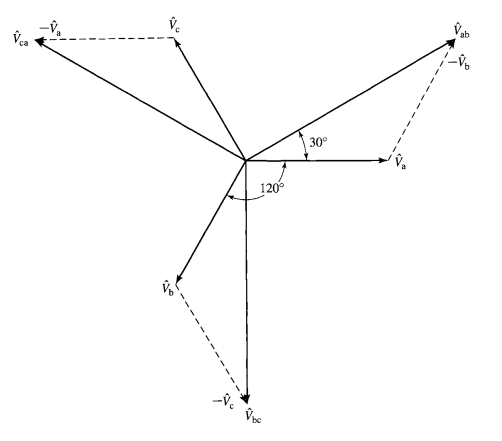
\includegraphics[width=0.4\linewidth]{Screenshots/wye_phasor}
		\caption{Wye Phasor Diagram (V)}
		\label{fig:wyephasor}
	\end{figure}
	\item \textbf{Delta-Connected:} When the three phases are Delta connected, the corresponding phasor diagram of currents is given in figure \ref{fig:deltaphasor}.
	\begin{figure}[h]
		\centering
		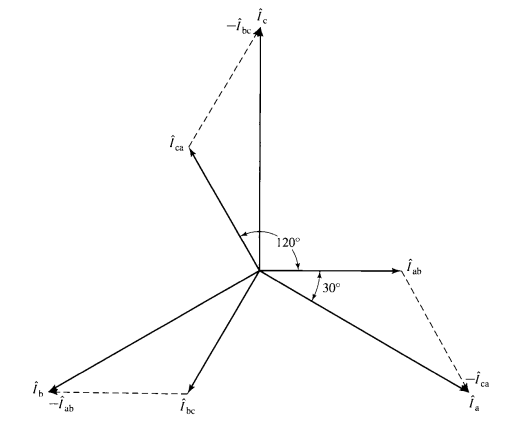
\includegraphics[width=0.4\linewidth]{Screenshots/delta_phasor}
		\caption{Delta Phasor Diagram (I)}
		\label{fig:deltaphasor}
	\end{figure}
	
	By KVL, the delta currents are: $\hat{I}_{ab}$, $\hat{I}_{bc}$ and $\hat{I}_{ca}$. By Kirchoffs current law:
	
	\begin{align*}
		\hat{I}_a = \hat{I}_{ab} - \hat{I}_{ca} = \sqrt{3}\hat{I}_{ab} \angle-30
	\end{align*}
	
\end{itemize}
\subsection{Balanced Loads Continued}

In analysis of a three-phase equivalent circuit, the recommended steps are:

\begin{enumerate}
	\item Construct a phasor diagram containing the AC phase voltages and the line voltages.
	\item Depending on wheter the system is a wye or delta connection, different approaches can be taken to analyze the load current and voltages. 
	\begin{enumerate}
		\item For \textbf{Wye} connections: It is possible to find the magnitudes via an equivalent circuit, containing a phase and an assumed neutral, as each load current and voltage is equivalent. We therefore isolate this single branch in an equivalent circuit and once the magnitudes are found, calculate phase angles.
		\item  Delta and Wye connections are essentially equivalent, except definitons for \textit{line to line} voltages change. Other than that, we can repeat the same equivalence process as we did with Wye connections, so long as the circuit is balanced and thus presence of a neutral line does not affect operating conditions. 
	\end{enumerate}
\end{enumerate}

Thus, we can interpret two important collararies based upon this equivalence:

\begin{enumerate}
	\item A general computation scheme for balanced circuits can be based entirely on Y-connected circuits or entirely on delta connected circuits.
	\item In frequently occuring problems in which the connection is not specified and not pertinent to the solution, either Y or delta connections can be used, such as in the analysis of three-phase motor performance.
\end{enumerate}

\textbf{Is there a correlation between reflected vectors and balanced phasors?}
	

\section{Week 6: Power in AC Loads}

Power in AC circuits with energy storage passive components is much more complex then in DC applications, because the power in these components is constantly being charged (absorbing, positive power) and discharged (supplying, negative power, in context of a circuit). In most applications domestic applications (washing machines, air conditioners, and refridgerators) are inductive in nature, and operate at a low lagging power factor.

\subsection{Average/True Power:}
The AC voltage that is applied to an AC load will result in AC current flowing due to a load impedance Z. We can describe this with:
\begin{align*}
	V &= |V| cos(\omega t + \phi _V) \\
	I &= |I|cos(\omega t + \phi_I)
\end{align*}
Where the phase difference $\phi = \phi_V - \phi_I$ describes the angle between the current and voltage.
Thus, the \textbf{average real power} is given either by:
\begin{align*}
	P_{rms} &= V_{rms} I_{rms} cos(\phi_V - \phi_I) = V_{rms} I_{rms} cos(\phi) \\
	P_{avg} &= \frac{1}{2} V I cos(\phi_V - \phi_I) = V I cos(\phi) = \frac{1}{2}I_0 ^2 |R| = \frac{1}{2} \frac{V_0}{|R|}^2
\end{align*}

\subsection{Reactive Power:} Reactive power is the complex portion of power in a load. Thus it is defiend as:
\begin{align*}
	Q_{rms} &= V_{rms} I_{rms} sin(\phi) = I_{rms}^2 X_c =  V_{rms}^2 X\\
	Q_{avg} &= \frac{1}{2} V I = V^2 / 2X_c = I^2X_c / 2 	\\
	Q &= \frac{1}{2}|V||I| sin (\phi)
\end{align*}
\subsection{Apparent Power:}
The apparent power is defined as the total power delivered to a load impedance, including reactive power losses. We describe this with:
\begin{align*}
	S_{avg}&=\frac{1}{2} I_0 V_0  = \frac{1}{2} I_0 ^2|Z| = \frac{1}{2} \frac{V_0 ^2}{|Z|} = \frac{P}{cos(\phi)} \\
	S_{rms}&= \frac{1}{2} I_0 V_0 sin(\phi_v - \phi_i) = \frac{1}{2}I_0^2 X = \frac{1}{2}V_0^2 B
\end{align*}

\subsection{Power Factor}
The power factor is a parameter that is frequently used to describe the efficiency of a circuit, and is given by:

\begin{align*}
	S &= \sqrt{Q^2 + X^2} \\
	\text{PF} &= cos(\phi_v - \phi_i)
\end{align*}

The power factor of a balanced three-phase system is equal to that of any one phase, that is:

\begin{align*}
	\theta = tan^{-1} \frac{X_p}{R_p} = cos^{-1} \frac{R_p}{Z_p} = sin^{-1} \frac{X_p}{Z_p}
\end{align*}

\subsection{Capacitive and Inductive Loads}

As discussed in the review section, capacitors and inductors have a complex impedance that defines the ratio of voltage to current at any given point in time, given a distinct frequency. We can use these relations to 'balance loads'. This is achieved by making Q (reactive power) sum to zero. Thus;

\begin{itemize}
	\item Capacitive loads can be balanced with inductors in paralell, or inductive with capacitors in parallel via:
	\begin{align*}
		Q_{circuit} &= S sin \phi \\
		X_c = \frac{V_{s}^2}{Q_b} &= I_s^2 Q_b \\
		\sum \frac{V_s^2}{X} &= Q_{circuit} + Q_b =  0
	\end{align*}
\end{itemize}

\section{Week 7: Electromagnetic Waves in Lossy Media}

\subsection{The Behaviour of Electrical and Magnetic Fields Through Differing Media}

The ability for electrical and magnetic fields to establish themselves in differing media is determined by an empirical constant, denoted $\epsilon_0$ and $\mu_0$ for electrical and magnetic fields respectively. This physical fact is used to contain electrical and magnetic fields in engineered geometries, such as motors, generators, transformers, and circuitry in general.
\newline
Maxwells equation, manilpulated to time-varying form describe self-sustaining, oscillating electromagnetic fields, which manifest themselves in many forms, from energetic gamma rays used in medical applications, to visibile light and through to radiowaves that carry information through space. We shall focus our attention on the simplest form of electromagnetic waves, that is unbounded electromagnetic plane waves. It is assumed that analysis is taken place at large distances relative to the source, such that the electromagnetic wave spans a "plane". 
\newline

\subsection{Representations of Maxwells Equations}
It is important to initially define mathematical model in which we can explain time-varying electromagnetic fields. The vector phasor:

\begin{align*}
	E(x,y,z,t) &= \Re [\vec{E} (x,y,z)e^{j\omega t}]
\end{align*} 
It becomes more obvious when we describe these phasors next to the time-domain representation:

\begin{figure}
	\centering
	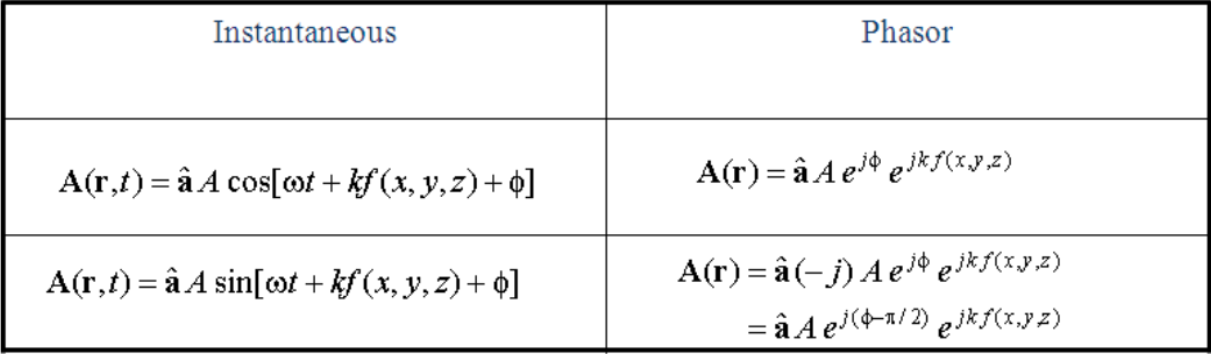
\includegraphics[width=0.5\linewidth]{Screenshots/phasor}
	\caption{Phasor Forms}
	\label{fig:phasor}
\end{figure}

Similar defintions apply to $\vec{D}$, $\vec{B}$ and $\vec{H}$. As well as to densities $\rho_v$ and $\vec{J}$. For a linear, isotropic and homogeneous medium with electrical permitivity $\epsilon$, magnetic permeability $\mu$ and conductivity $\sigma$, Maxwell's equations assume:

\begin{align}
	\nabla \cdot \vec{E} &= \vec{\rho}_v / \epsilon \\
	\nabla \times \vec{E} &= - j\omega \mu \vec{H} \\ 
	\nabla \cdot \vec{H} &= 0 \\
	\nabla \times \vec{H} &= \vec{J} + j\omega \epsilon \vec{E}
\end{align} 

Tabulating these results for source free fields, which satisfy the condition: $\rho_v = 0$, that is there are no conductive sources within the media;

\begin{figure}[h]
	\centering
	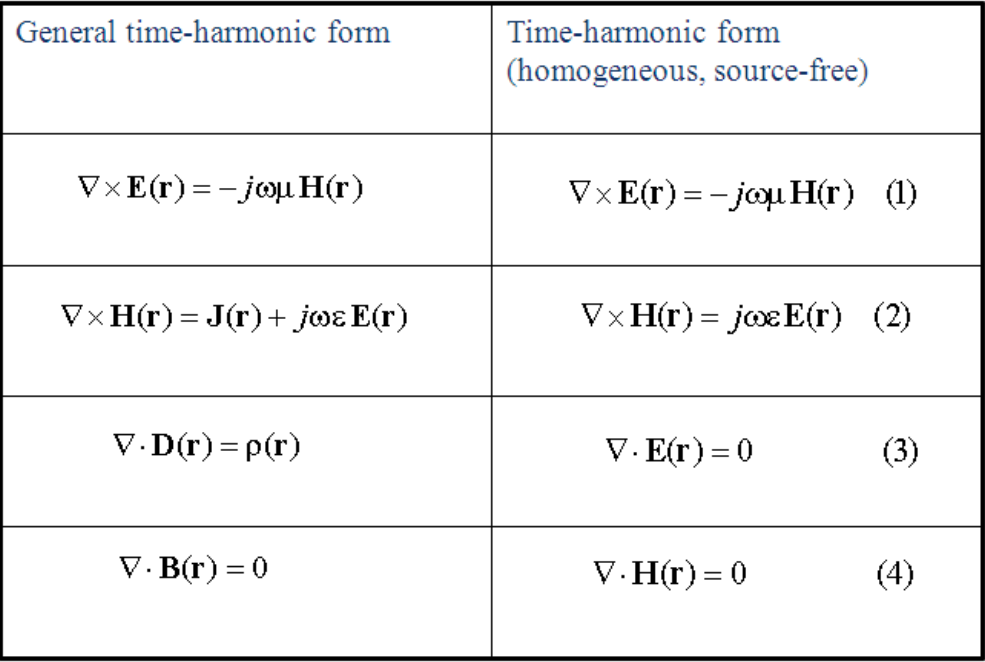
\includegraphics[width=0.5\linewidth]{Screenshots/phasor_maxwells_equations}
	\caption{Phasor Form of Maxwells Equations}
	\label{fig:phasormaxwellsequations}
\end{figure}


Here, we will use Faradays law of induction (1), Amperes law (2) and Gauss's law (3) to derive a solution of the wave equation:

\begin{itemize}
	\item Take the curl of (1), and use (3) to sub into (2):
	\begin{align*}
		\text{LHS: } \nabla  \times \nabla \times \vec{E} &= \nabla (\nabla \dot \vec{E}) - \nabla^2 \vec{E} = 0-\nabla^2\vec{E} \\
		\text{RHS: } -j\omega \mu (\nabla \times \vec{H}) &= -j \omega \mu (j\omega \epsilon \vec{E}) = \omega^2 \mu \epsilon \vec{E} 
	\end{align*}
	\item Which gives us the homogeneous wave equation:
	\begin{align*}
		\nabla^2 \vec{E}(\vec{r}) +k^2 \vec{E}(\vec{r}) &= 0
	\end{align*}
	\item  Let $k=\omega \sqrt{\mu \epsilon}$ \textbf{(wavenumber)}, and considering a simple case where $\vec{E}(\vec{r}) = \hat{x} E_x (z)$. The wave equation reduces to:
	\begin{align*}
		\frac{d^2 E_x(z)}{dz^2} + k^2 E_x(z)=0
	\end{align*}
	The solution of this equation is given solving for the characterisitic polynomials, which turn out to be $\lambda=\pm jk$ by:
	\begin{align*}
		E_x (z) &= E_0 ^+ e^{-jkz} + E_0^- e^{+jkz} = E_x^+ + E_x ^-(z) 
	\end{align*}
	Which can be put into instantaneous expressions via the identities above. For a brief intuition, see the figure below:
	
	\begin{figure}[h]
		\centering
		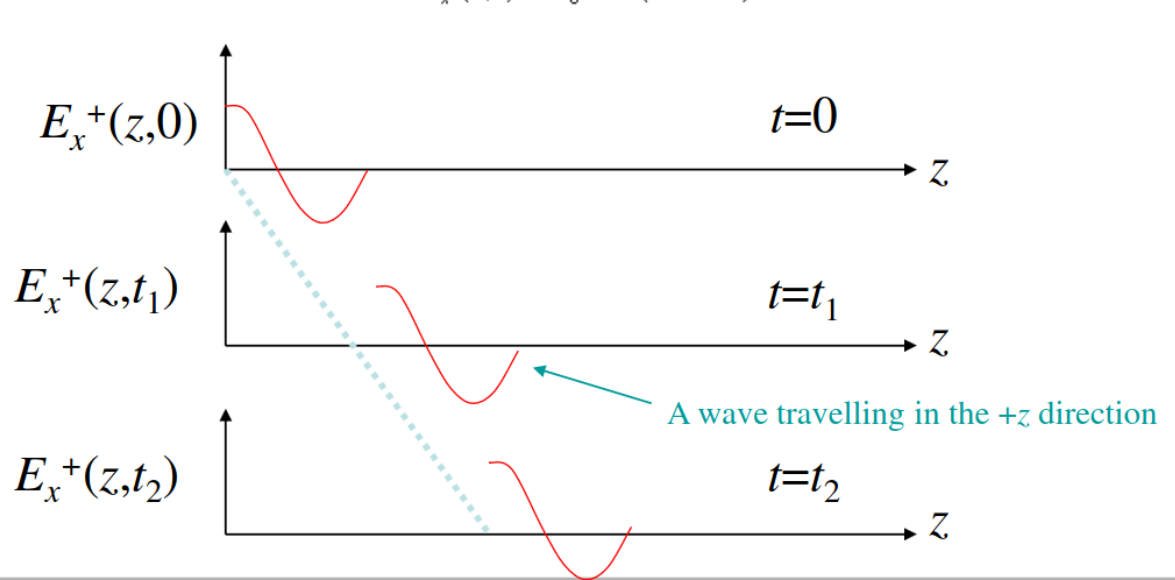
\includegraphics[width=0.5\linewidth]{Screenshots/phasor2}
		\caption{Plot of Simplified Wave Equation Solution}
		\label{fig:phasor2}
	\end{figure}
\end{itemize}

For each wave travelling within a medium there are a range of parameters that are necessary to model its behaviour. They are listed below:

\begin{align*}
	\beta &= k = \omega \sqrt{\mu \epsilon} \\
	\lambda &= \frac{2\pi}{\beta} = \frac{\mu_p}{f} \\
	\mu_p &= \frac{1}{\sqrt{\mu \epsilon}} = \frac{\omega}{\beta} \\
 \eta & = \sqrt{\frac{\mu}{\epsilon}} \text{ (Intrinsic Imepdance)}
\end{align*}
We shall see, when considering large enough conductors, such as transmission lines, in which the AC wavelength is on the same scale as the length of the conductor, can also be described by an analog to intrinsic impedance of a lossless medium.

\begin{figure}[h]
	\centering
	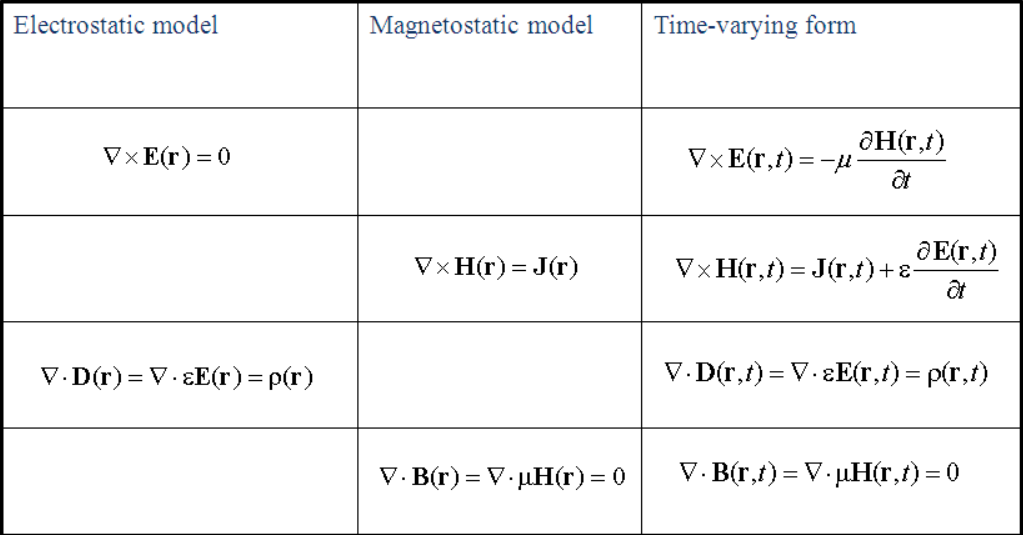
\includegraphics[width=0.7\linewidth]{Screenshots/maxwells_equations}
	\caption{Maxwells Equations}
	\label{fig:maxwellsequations}
\end{figure}

Maxwell's equations in differential form, summarised by table \ref{fig:maxwellsequations}, can be rewritten in terms of \textbf{source-free space}.

\begin{align*}
	\nabla \times \vec{E}(r,t) &= -\mu \frac{\delta \vec{H}(\vec{r},t)}{\delta t} \text{ (Faraday's Law of Induction)}\\
	\nabla \times \vec{H}(r,t) &= \epsilon \frac{\delta \vec{E} (\vec{r}, t)}{\delta t} \text{ (Ampere's Law)}\\
	\nabla \cdot \vec{E}(\vec{r}, t) &= 0 \text{ (Gauss's law)} \\
	\nabla \cdot \vec{H}(\vec{r}, t) &= 0 \text{ (Gauss's law of Magnetism)}
\end{align*}

These equations describe the ability of an electromagnetic wave to sustain itself in a medium regardless of any source nearby. We can derive the functions describing the relation between electric and magnetic field of a given plane wave simply using Faradays law.

\begin{align*}
	\nabla \times \vec{E}(r,t) &= -\mu \frac{\delta \vec{H}(\vec{r},t)}{\delta t} \\
	\begin{bmatrix}
		\hat{i} & \hat{j} & \hat{k} \\
		\delta/\delta x & \delta/\delta{y} & \delta/\delta{z}\\
		E_x(z) &0 & 0 \\
	\end{bmatrix}&= -j\omega \mu (\hat{u}\vec{H}(\vec{r})) \\
	\text{OR:  }&\\
	\vec{H} &= \frac{1}{\eta} \hat{k} \times \vec{E} \\
	\vec{E} &= -\eta \hat{k} \times \vec{H}
\end{align*}
Where $\hat{u}$ and $\vec{r}$ are simply general expressions to denote the direction of the magnetic field and propogation respectively. The expression for electromagnetic waves here is called \textbf{TEM} electromagnetic, and is not valid for other types of emw polarization. 

 This forms the foundation of man-kinds \textbf{classical} understanding of photons, and it is a good model on most occasions, except the model begins to breakdown when we consider:

\begin{itemize}
	\item When describing the photoelectric effect.
	\item The behaviour of electrons 'orbiting a nucleus'
	\item The effects of blackbody radiation.
	\item Relativistic models.
	\item Pair production.
\end{itemize}

However for our purposes at the moment these considerations \textbf{do not} come into view. We will describe the classical model of electromagnetism which is appropriate for most electrical engineering applications.

\begin{figure}
	\centering
	\includegraphics[width=0.6\linewidth]{../Assessment/wave_params}
	\caption{Wave Parameters Tabulated	}
	\label{fig:waveparams}
\end{figure}

\subsection{Wave Polarization:}

The polarization of a uniform plane wave describes the locus traced by the tip of the $\vec{E}$ vector in the plane orthogonal to direction of propagation, as some point in time $t$. There are a couple of general types plane-wave propogation polarization models generated by different man-made antennas:

\begin{itemize}
	\item Elliptical LHC polarization.
	\item Elliptical RHC polarization
\end{itemize}

In any case, the inclination angle $\Psi$ determines the angle between arbitrary orthagonal axes (obviously w.r.t one or the other):

\begin{align*}
	\Phi(z,t) = tan^{-1}[\frac{E_y(z,t)}{E_x(z,t)}]
\end{align*}

And the polarization type can be determined via the angle relations determined directly from the field equations. (pg 331, Umberto).

\section{Week 8: Plane Waves in Media}

In practice, all mediums suffer loss. This includes air. A brief summary of the notation used will be listed below.

\begin{itemize}
	\item Lossless dielectric medium $\epsilon_r$, $\mu_r$, real.
	\item Nonmagnetic medium, $\mu_r=1$
	\item Lossy media: $\epsilon= \epsilon_r' - j\epsilon_r ''$ complex, $\epsilon_r '$ and $\epsilon_r ''$ positive real.
	\item Permittivity of lossy media: $\epsilon = \epsilon_r \epsilon_0 = (\epsilon_r' - j\epsilon_r '') \epsilon_0$
	\item Other ways of specifying lossy media:
	\begin{itemize}
		\item In terms of $\epsilon_r$, which is actually $\epsilon_r'$ and $\sigma = \omega \epsilon''$.
		\item In terms of $\epsilon_r$, which is actually $\epsilon_r'$ and $tan\delta=\epsilon''/\epsilon'=\sigma/(\omega \epsilon_0 \epsilon_r ')$.
	\end{itemize} 
	\item Complex permeability $\mu=\mu'-j\mu''$.
	\item In practice, $\mu ' >> \mu ''$.
	\item Therefore $\mu = \mu ' = \mu_r \mu_0$
\end{itemize}


\subsection{Lossy Media}
Essentially all of this information can be encapsulated within the propagation constant $\gamma = \alpha + j \beta$. I.e:

\begin{align*}
	\nabla^2 \vec{E} - \gamma^2 \vec{E} &= 0 \\
	\gamma^2 = -\omega^2 \mu \epsilon_c = \omega^2 \mu (\epsilon' - j\epsilon'')
\end{align*}

Solving with $\gamma = \alpha + j \beta$ for $\alpha$ and $\beta$ in lossy media yields:

\begin{align*}
	\alpha &= \omega ({ \frac{\mu \epsilon'}{2} [\sqrt{1 + (\frac{\epsilon ''}{\epsilon})} -1]})^{1/2} \\
	\beta &= \omega ({ \frac{\mu \epsilon'}{2} [ \sqrt{1+ (\frac{\epsilon ''}{\epsilon})} + 1]})^{1/2} 
\end{align*} 

The associated magnetic field can be determined if the electric field is known, and vice versa through the relations:

\begin{align*}
	\vec{E}(z) &= \hat{x} \vec{E}_{0} e^{-\gamma z} = \hat{x} \vec{E}_{0} e^{-\alpha z}e^{-j \beta z} \\
	\vec{H}(z) &= \hat{y} \frac{\vec{E}_{0}}{\eta_c} e^{-\gamma z}	= \hat{y} \frac{\vec{E}_{0}}{\eta_c} e^{-\alpha z}e^{-j \beta z}
\end{align*}


\subsection{Varying Permittivity, Permeability}
In a lossless dielectric medium, the relative permittivity $\epsilon_r$ is real. For non-magnetic materials, the relative permeability is $\mu_r = 1$. For \textbf{lossy media}, $\epsilon_r = \epsilon_r ' - j\epsilon_r''$ is a complex number where $\epsilon_r'$ and $\epsilon''$ are positive real quantities. We often use the following equations to describe the materials:
\begin{itemize}
	\item $\sigma = \omega \epsilon''$ (Equivalent Conductivity)
	\item $\epsilon'' = \frac{\sigma}{\omega \epsilon_0}$
	\item $\epsilon'' / \epsilon' = \sigma/\omega \epsilon$
\end{itemize}


Similar arguments apply for the permeability, which may also be complex. I.e, $\mu = \mu ' - j \mu''$. However, in practice, $\mu ' >> \mu ''$, and therefore $\mu \approx \mu' = \mu_r \mu_0$ for most materials. As we shall see, this results in a \textbf{complex intrinsic impedance}, thus meaning the electric and magnetic fields will be out of phase.

In any medium, electromagnetic fields must always satisfy Maxwells equations. Assuming sinusoidal time dependence, we make use of the complex vector notation to solving the Eigenvalue problem for the homogeneous vector Helmholtz equation:
\begin{align*}
	\nabla^2\vec{E} (x,y,z)+k^2\vec{E}(x,y,z)=0
\end{align*}
Where $k=\omega\sqrt{\mu \epsilon}$. For a lossy medium, $k$ becomes complex:
\begin{align*}
	k\sqrt{\mu\epsilon} &= \omega \sqrt{\mu_0 \epsilon_0} \sqrt{\mu_r \epsilon_r} \\
	&=k_0 \sqrt{\mu_r (\epsilon'-j\epsilon''_r)} \\
	&= \beta - ja
\end{align*}
Where $\beta$ and $a$ are the phase and attenuation constants, measured in radians per metre and nepers per metre. Both are positive constants.
\begin{itemize}
	\item It is important to note that the neper is defined as a logarithmic constant, that is 1 neper is $8.688$dB. An attenuation of $\alpha$ Np/m equals $-20log(e^{-\alpha})=8.686 \alpha $dB/m.
\end{itemize}

As in the lossless case, the electric field phasor of a plane wave propogating in the lossy medium in a direction $\hat{a}_n$ and polarisation $\vec{e}$ may be expressed as:
\begin{align*}
	\vec{E}(\vec{r}) &= \hat{e} E_0 e^{-jk \hat{a}_n \cdot \vec{r}} \\
	&= \hat{e} |E_0| e^{j\phi} e^{-\alpha(\hat{a}_n \cdot \vec{r})}e^{-j \beta (\hat{a} \cdot \vec{r})}
\end{align*}

Where $E_0 = |E_0| e^{j \phi}$. Figure [\ref{fig:lossymedia}] describes the effect of equivalent conductivity ($\sigma= \omega \epsilon''$). We can derive an expression for the magnetic field via Faradays law:
\begin{align*}
	\vec{H} (\vec{r},t) = Re[\vec{H}(\vec{r})e^j\omega t] = (\hat{a}_n \times \hat{e}) \frac{|E_0|}{|n|} e^{-a(\hat{a}_n \cdot \vec{r})} cos(\omega t - \beta(\hat{a}_n \cdot \vec{r} + \phi - \theta))
\end{align*}

\begin{figure}[h]
	\centering
	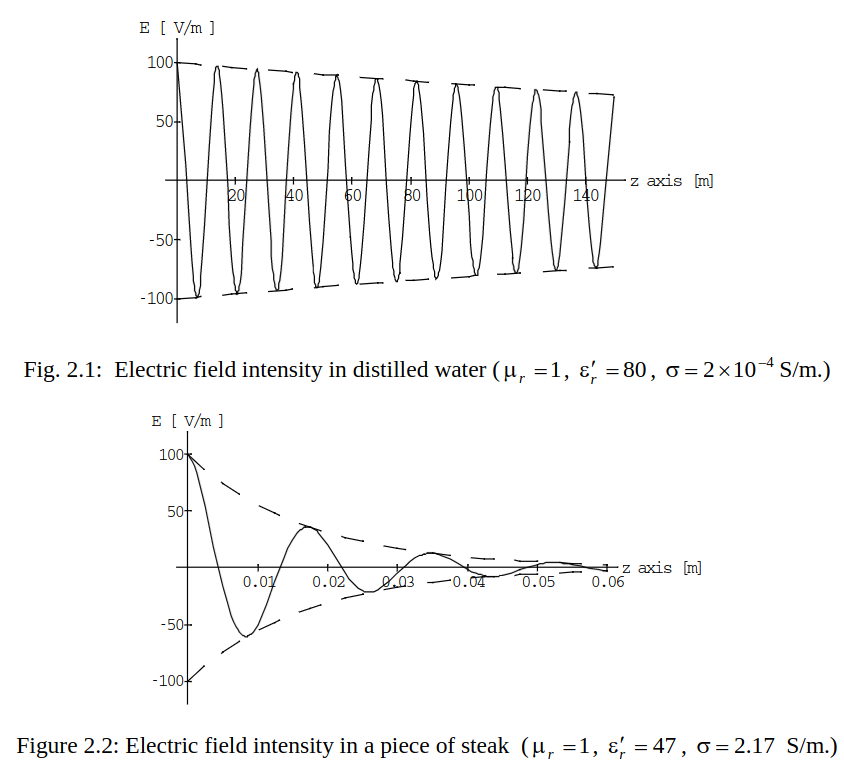
\includegraphics[width=0.6\linewidth]{Screenshots/lossy_media}
	\caption{Lossy Media}
	\label{fig:lossymedia}
\end{figure}

\subsection{Approximations for low-loss dielectrics and good conductors}

For certain materials, it is possible to calculate approximate values for $\beta$, $\alpha$ and $n$ using closed form equations, i.e, without having to compute the square root of a complex number. 

\begin{figure}[h]
	\centering
	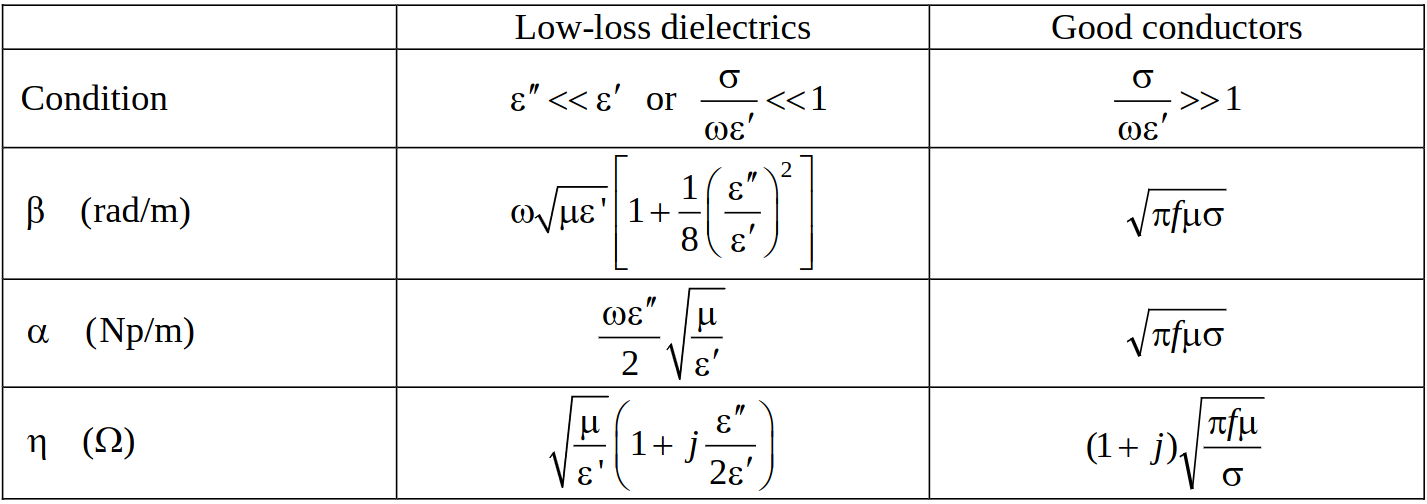
\includegraphics[width=0.6\linewidth]{Screenshots/approximations_for_good_conductors}
	\caption{Tabulated Approximations For $\beta$, $\alpha$, $n$ for low loss dielectrics and good conductors.}
	\label{fig:approximationsforgoodconductors}
\end{figure}

\begin{figure}[h]
	\centering
	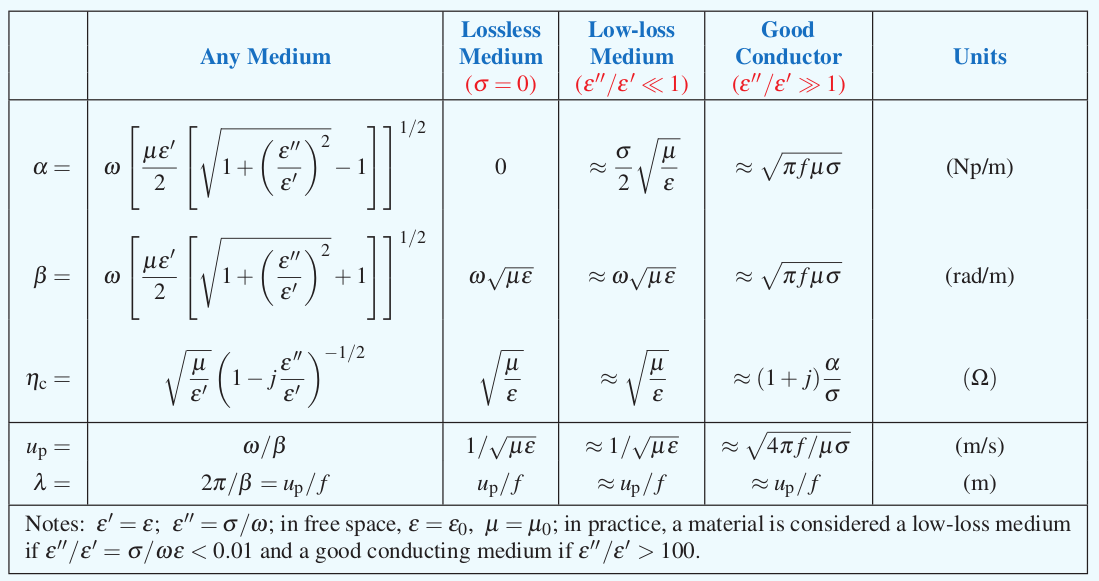
\includegraphics[width=0.5\linewidth]{Screenshots/tabulated_expressions_2}
	\caption{Tabulated Expressions for Differing Media}
	\label{fig:tabulatedexpressions2}
\end{figure}


These expressions arise by the necessity to classify how lossy a system is/

\subsection{Wave Polarization}

The polarization of a uniform plane wave describes the locus traced by the tip of the $\vec{E}$ vector (in the plane orthogonal to the direction of propagation) at a given point in space as a function of time. There are thus various polarization types:

\begin{itemize}
	\item \textbf{Elliptically polarized}: If the tip of $\vec{E}$ is an ellipse,the wave is said to be elliptically polarized.
\end{itemize}


\subsection{Skin depth/depth of penetration}

Since the attenuation factor is $I / I_0 = e^{-az}$, the amplitude of a wave will be attenuated by a factor of $e^{-1}=0.368$ when it travels a distance of $\delta = 1/\alpha$. This is called the skin depth or depth of penetration. For higher frequencies (such as microwave frequencies), the skin depth of a good conductor is so small that fields and currents can be considered as, for all practical purposes, confined to a very thin layer (i.e the skin) of the conductor surface. 



\begin{figure}[h]
	\centering
	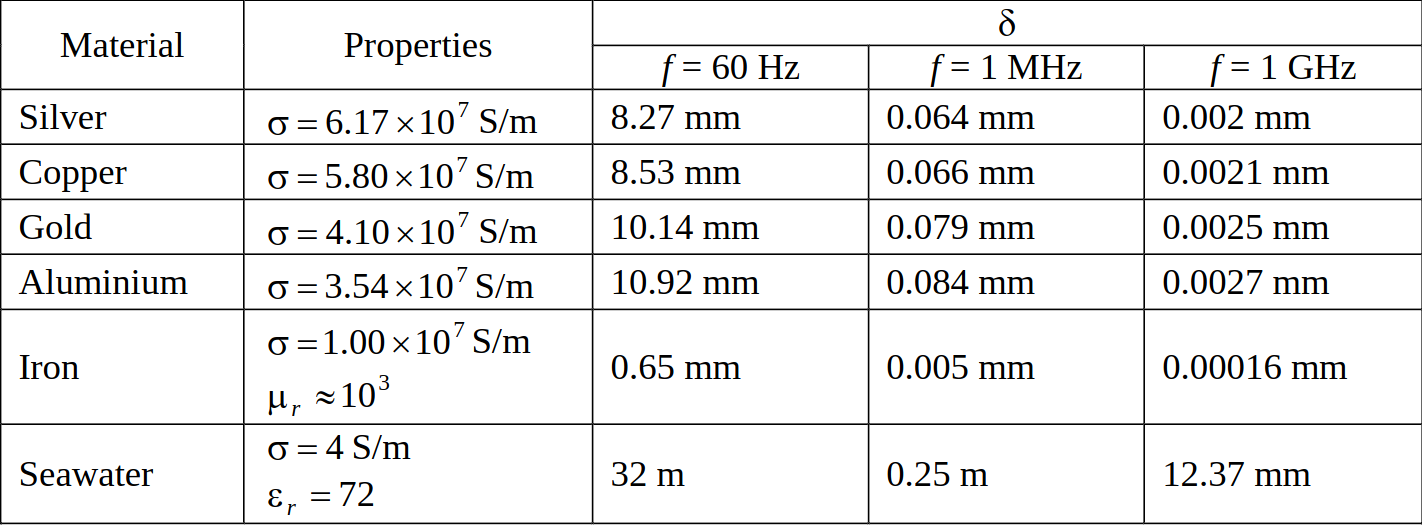
\includegraphics[width=0.5\linewidth]{Screenshots/skin_depth_of_materials}
	\caption{Skin Depth of Materials at Certain Frequencies}
	\label{fig:skindepthofmaterials}
\end{figure}

In particular cases, when the low loss and good conductor characteristics ratios are close to one, then we can use the fact that $k= \beta - j \alpha$ to determine the $\delta= \alpha^{-1}$.

\subsection{Flow of Electromagnetic Power and the Poynting Vector}

Electromagnetic waves can carry unimpeded energy through space, able to induce currents and voltages a long distance away from its source. Consider an arbitrary electromagnetic field, ($\vec{E}(\vec{r}, t), \vec{H}(\vec{r},t)$) in a simple medium whose constitutive parameters $\epsilon$, $\mu$, and $\sigma$ do not change with time. If we start with Maxwell's equations:

\begin{align*}
	\nabla \times \vec{E}(r,t) = -\mu \frac{\delta H(\vec{r}, t)}{\delta t}
\end{align*}

and 

\begin{align*}
	\nabla \times \vec{H}(r,t) = \vec{J}(\vec{r},t) + \epsilon \frac{\delta E(\vec{r}, t)}{\delta t} = \sigma \vec{E}(\vec{r}, t)+ \epsilon \frac{\delta \vec{E}(\vec{r}, t)}{\delta t}
\end{align*}

We can use identities of vector operations to show that:

\begin{align*}
	\nabla \cdot [\vec{E}(\vec{r},t) \times \vec{H}(\vec{r}, t)] = -\frac{\delta}{\delta t} (\frac{1}{2} \epsilon E^2) - \frac{\delta}{\delta t} (\frac{1}{2}\mu H^2) - \sigma E^2
\end{align*}

Where 
\begin{align*}
	E^2 = |\vec{E}(r,t)|^2 = \vec{E}(\vec{r}, t) \cdot \vec{E}(\vec{r}, t)
\end{align*}
and 
\begin{align*}
	H^2 = |\vec{H}(\vec{r}, t)|^2 = \vec{H}(\vec{r}, t) \cdot \vec{H} (\vec{r}, t)
\end{align*}

If we integrate over both sides of the rate of change energy density equation, over a volume V, and use the divergence theorem to convert a contour integral to a closed surface integral, then we obtain:

\begin{align*}
	-\oint\vec{S} (\vec{r}, t) \cdot ds = \frac{\delta}{\delta t} \int_{V} w_e dv + \frac{\delta}{\delta t} \int_{V}w_m dv + \int_{V}\sigma \vec{E}^2 dv
\end{align*}
Where:
\begin{itemize}
	\item $w_e = 1/2 \epsilon E^2$ is the stored electric energy density.
	\item $w_m = 1/2 \mu H^2$ is the stored magnetic energy density
	\item $\sigma E^2$ is the Ohmic power density. 
\end{itemize}
This refers to Poyntings theorem. It states the the total power flowing into a closed surface at any instant equals the sum of the rate of increase in the stored electric and magnetic energy and the ohmic power dissipated within the enclosed volume. This allows use to arrive at the Poynting vector:

\begin{align*}
	\vec{S}(\vec{r}, t) = \vec{E}(\vec{r}, t) \times \vec{H} (\vec{r}, t)
\end{align*}

If we calculate the Poynting vector of a plane wave, we will see that the direction of power flow will always be in the direction of propagation. The instanteous power density is not particularly useful. We instead can gain more insight when considering its average, 

\begin{align*}
	\vec{S}_{av} (\vec{r}) = \frac{1}{T} \int_{0}^{T} \vec{S}(\vec{r}, t)dt
\end{align*}

Furthermore, we can express average power density using phasor expressions:

\begin{align*}
	\vec{S}_{av}(\vec{r}) = \frac{1}{2} Re [\vec{E} (\vec{r}) \times \vec{H}(\vec{r})]
\end{align*}

\textbf{Average Power in W/m$^2$}
\begin{itemize}
	\item \textbf{Power in Lossless Media:}
	\begin{align*}
		\vec{S}_{av} = \hat{z} \frac{1}{2\eta}(|E_x0|^2 + |E_y|^2) =\hat{z} \frac{|\vec{E}|^2}{2\eta}  
	\end{align*}
	\item \textbf{Power In Lossy Media:}
	\begin{align*}
		\vec{S}_{av} = \hat{z} \frac{1}{2\eta}(|E(0)|^2 + |E_y|^2)  e^{-2az} cos \theta_{\eta}   
	\end{align*}

\end{itemize}

\subsection{Flow of Electromagnetic Fields in Lossy Media}

It was shown in lossy media representations of electromagnetic plane waves needed to be generalised to fit the behaviour of propogation. Thus we define a the propagation constant $\gamma = \alpha + j \beta$. By extending these expressions to the more general case of a wave with components along both x and y, we have:

\begin{align*}
	\vec{E}(z) &= \hat{x} E_x (z) + E_y (z) = (\hat{x} E_x  + \hat{y} E_y ) e^{-\alpha z} e^{-j\beta z} \\
	\vec{H}(z) &=\frac{1}{\eta_c} (\hat{x} E_x 0 + \hat{y} E_y0 ) e^{-\alpha z} e^{-j\beta z}
\end{align*} 

Which defines the equations for electric and magnetic fields in lossy media. We see: What are we supposed to see?

\subsection{Summary}

Transverse electromagnetic waves are relatively easy to deal with. We can make various assumptions, and describe invisible electromagnetic waves with the simple TEM model (that is, the electric and magnetic fields are orthogonal to one another). The magnitudes of these fields are plainly related by the intrinsic impedance of the media. We shall see that the power density described the TEM wave is akin to that of the power travelling in a transmission line.

\section{Week 9: Reflection and Absorption for Electromagnetic Plane waves}


\begin{itemize}
	\item Reflection occurs when an electromagnetic wave travelling in one medium impinges on another with a different intrinsic impedance. This behaviour differs depending on whether the boundary is conducting, or dielectric.
	\item Application of Gauss's law for and Gauss's law for magnetism for a pillbox straddling two adjacent, continuous media (page 270), Umberto Ravaioli, yields:
	
	\begin{align*}
		\oint_S \vec{E} \cdot dS &= Q \xrightarrow{} D_{a} - {D_b} = \rho_s \\
		\oint_S \vec{B} \cdot d\vec{s} &= 0 \xrightarrow{}  B_a = B_b
	\end{align*}
	Inspection of this result for magnetism shows that the normal component of $\vec{B}$ is continuous across the boundary between two adjacent media. Although this is electro / magnetostatics, it is important to keep this in mind when considering time-varying electric and magnetic fields travelling into new media.
\end{itemize}

\begin{figure}[h]
	\centering
	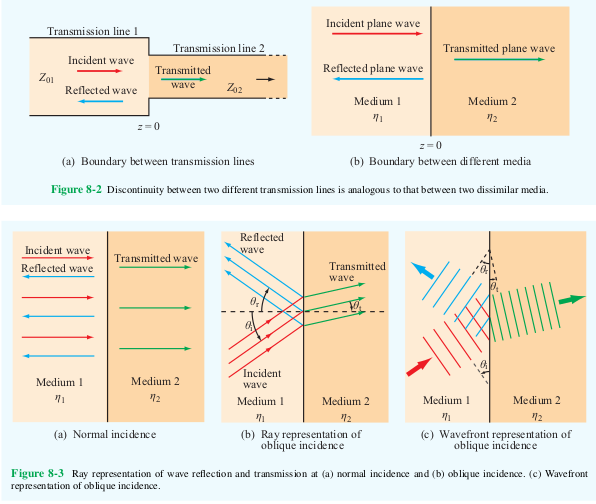
\includegraphics[width=0.5\linewidth]{Screenshots/emw_behaviour_different_media}
	\caption{EMW Behaviour in Differing Media}
	\label{fig:emwbehaviourdifferentmedia}
\end{figure}

Figure \ref{fig:emwbehaviourdifferentmedia} encapsulates a range of models used to describe the behaviour of electromagnetic waves on different media. 

\subsection{Normal Incidence, Lossless Media:}

The behaviour of reflected emws in lossless media, such as air or conductors (approximately) is described by:

\begin{figure}[h]
	\centering
	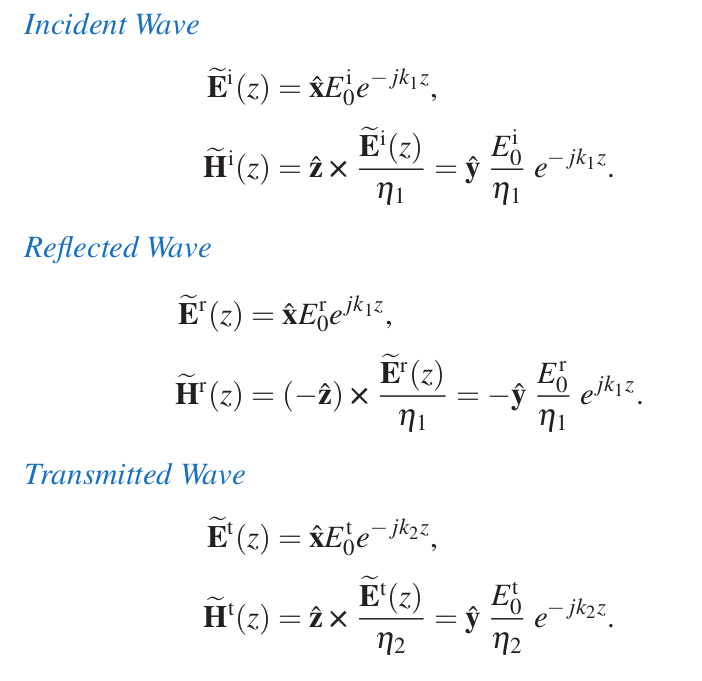
\includegraphics[width=0.4\linewidth]{Screenshots/emw_behaviour_different_media1}
	\caption{Incident Waves}
	\label{fig:emwbehaviourdifferentmedia1}
\end{figure}

We can further model these equations with:

\begin{align*}
	\Gamma &= \frac{E_0^r}{E_0^i} = \frac{\eta_2 - \eta_1}{\eta_2 + \eta_1} \text{ (Reflection coefficent)} \\
	\tau  &= \frac{E_0^t}{E_0^i} = \frac{2\eta_2}{\eta_2 + \eta_1} \text{ (Transmission Coefficient)} \\
	\tau &= 1+\Gamma \text{ (Normal Incidence)}
\end{align*}

These reflections determine the percentage of electric field magnitude that is transmitted into or reflected from the incident material. These relations have direct analogs to transmission line theory, which is discussed next. 

\begin{figure}[h]
	\centering
	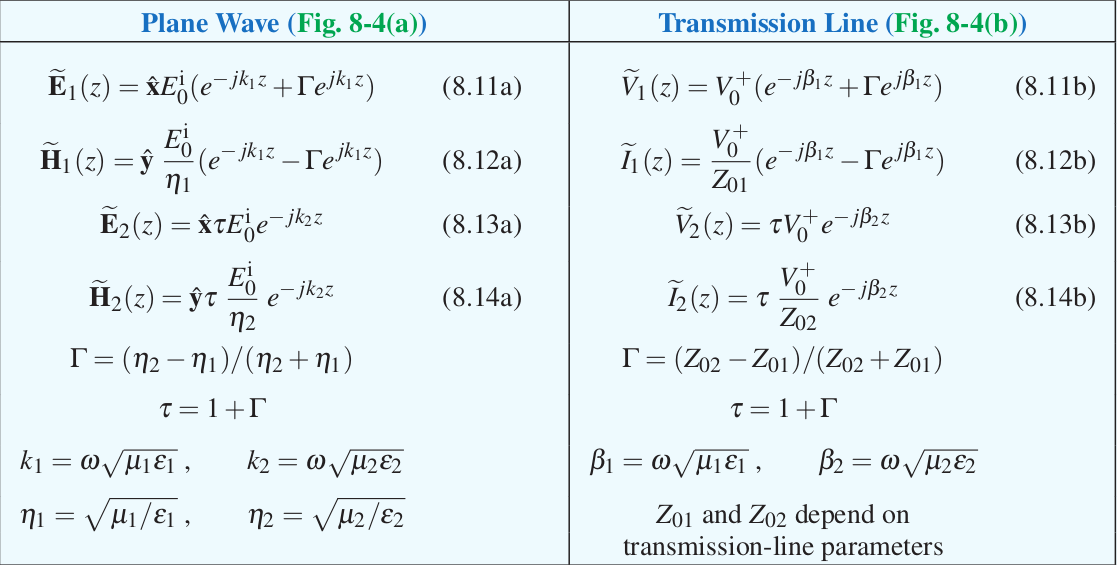
\includegraphics[width=0.5\linewidth]{Screenshots/plane_wave_transmission_line_analogy}
	\caption{Plane Wave / Transmission Line Analogs}
	\label{fig:planewavetransmissionlineanalogy}
\end{figure}

A parameter defined in transmission line theory, the standing wave ratio in a particular medium is defined as:

\begin{align*}
	S = \frac{|\vec{E}|_{max}}{|\vec{E}|_{min}} = \frac{1 + |\Gamma|}{1-|\Gamma|}
\end{align*}

Notice that if the two intrinsic impedances of the media match (as is the case with impedances in transmission line networks), the wave is not reflected and a standing wave is established, terminating completely in the load, ensuring maximum power transfer. 

\begin{align*}
	-z = I_{max} &= \frac{\theta_r + 2n\pi}{2k_1} = \frac{\sigma_r \lambda_1}{4 \pi} + \frac{n \lambda_1}{2} \\
	&= \begin{cases}
		n = 1,2,3... & \text{if } \theta_r < 0 \\
		n=0,1,2,... & \text{if } \theta_r \geq 0
	\end{cases}
\end{align*}

\subsection{Boundary Between Lossy Media}

We will have to generalize our parameters for normally incident plane waves between, to or from lossy media. In a medium with constiutive parameters $(\epsilon, \mu, \sigma)$, the propogation constant $\gamma = \alpha + j \beta$ and the intrinsic impedance $\eta_c$ are both complex. Therefore, we extend our formulations for lossy media:


\begin{figure}[h]
	\centering
	\includegraphics[width=0.5\linewidth]{Screenshots/lossy_media_incidence}
	\caption{Normal Incidence on Lossy Media}
	\label{fig:lossymediaincidence}
\end{figure}

\textbf{Medium 1}
\begin{align*}
	\vec{E}(z) &= \hat{x} E_0 ^i (e^{-\gamma_1 z + \Gamma e^{\gamma z}}) \\
	\vec{H}(z) &= \hat{y} \frac{E_0^i}{\nu_{c_1}} (e^{-\gamma_1z-\Gamma e^{\gamma_1z}})
\end{align*}

\subsection{Refelected and Transmitted Power Densities}

When normally incident waves are reflected off of a parcticular surface, their description for power densities becomes slightly more complex. 

\begin{itemize}
	\item \textbf{Lossless Media:} \newline	
	Media 1:
	\begin{align*}
		\vec{S}_{av1} &= \frac{1}{2} \text{Re}[\vec{E_1} (z) \times \vec{H}(z)] \\
		&= \hat{z} \frac{|E_0 ^i|^2}{2\eta_1} (1 - |\Gamma|^2) \\
	\end{align*}
	Media 2:
	\begin{align*}
		\vec{S}_{av2} &= \frac{1}{2} \text{Re}[\vec{E}_2 (z) \times \vec{H}_2(z)]\\
		&= |\tau|^2\frac{|E_0^i|^2}{2\eta_2} 
	\end{align*}
\end{itemize}

These expressions describe the average power densities of electromagnetic waves incident on some media. Note that if reflection and transmission coefficients asa known, as well as the incident source, it is easy to determine these power densities.

\subsection{Snells Laws - Wave reflection and Refraction}

When an electromagnetic wave is incident non-normally, or oblique incidence, we can represent its behaviour borrowing from optics and using Snells law. Snells law is essentially derived from Huygens principle, and it makes use of approximations according to far field radiation. It is left as an excercise to derive:

\begin{align*}
	\theta_i &= \theta_r  \text{ (Snells Law of Reflection)}\\
	\frac{sin \theta_t}{sin \theta_i} &= \frac{u_{p2}}{u_{p1}} = \sqrt{ \frac{\mu_1 \epsilon_1}{\mu_2 \epsilon_2}} \text{  (Snells Law of Refraction)} \\
	n &= \frac{c}{u_p} = \sqrt{\frac{\mu \epsilon}{\mu_0 \epsilon_0}} = \sqrt{\mu_r \epsilon_r}
\end{align*}

Combining these three equations for nonmagnetic materials, that is $\mu_{r1}$ = $\mu_{r2} = 1$;
\begin{align*}
	\frac{sin\theta_t}{sin\theta_i} = \frac{n_1}{n_2} = \sqrt{ \frac{ \epsilon_1}{\epsilon_2}} = \frac{\eta_2}{\eta_1} 
\end{align*}

These equations state that the angle of reflection equals the angle of incidence (reflection), and Snell's law of refraction provides a relation between $sin\theta_t$ and $sin\theta_i$ in terms of the ratio of the phase velocities.

This law is maintained in any form of incidence between two media. It can also be derived by considering the boundary conditions of the media.

\subsection{Aribitrary Polarization:}

A wave of arbitrary polarization can be broken into a superposition of two orthogonally polarized waves: one with its electric field parallel to the place of incidence and the other with its electric field perpendicular to the plane of incidence. 

\begin{figure}[h]
	\centering
	\includegraphics[width=0.2\linewidth]{Screenshots/incident_planes}
	\caption{Parallel and Perpendicular Plane Superposition}
	\label{fig:incidentplanes}
\end{figure}

A wave is:
\begin{itemize}
	\item \textbf{Perpendicularly Polarized:} When its $\vec{E}$ field is perpendicular to the plane of incidence.
	\item \textbf{Parrallel Polarized:} When its electric field vector lies in the plane of incidence.  
\end{itemize}

\begin{figure}[h]
	\centering
	\includegraphics[width=0.4\linewidth]{Screenshots/incident_planes1}
	\caption{Perpendicularly Polarized Plane Wave Incident at an angle $\theta_i$ upon a planar boundary}
	\label{fig:incidentplanes1}
\end{figure}

\begin{itemize}
	\item \textbf{Incident Wave}
	\begin{align*}
		\vec{E} _\perp &= \hat{y} E^i_{\perp 0} e^{-jk_1(xsin\theta_i +zcos\theta_i)} \\
		\vec{H}_\perp ^i &= (-\hat{x} cos\theta_i + \hat{z} sin\theta_i) \frac{E_{\perp0 }^i}{\eta _1} e^{-jk_1 (xsin\theta_i + z cos\theta_i)}
	\end{align*}
	\item \textbf{Reflected Wave}
	\begin{align*}
		\vec{E} _\perp &= \hat{y} \vec{E}_{\perp0} ^r\hat{y}e^{-jk_1 x_r} = E^r_{\perp 0} e^{-jk_1(xsin\theta_r -zcos\theta_r)} \\
		\vec{H}_\perp ^i &= \hat{y}_r \frac{E^r_{\perp0}}{\eta_1} e^{-jk_1 x_r} = (\hat{x} cos\theta_r + \hat{z} sin \theta_r) \frac{E_{\perp0}^r}{\eta_1} e^{-jk_1(xsin\theta_r - zcos\theta_r)}
	\end{align*}
	\item \textbf{Transmitted Wave}
	\begin{align*}
		\vec{E} _\perp^t &= \hat{y} \vec{E}_{\perp0} ^t\hat{y}e^{-jk_2 x_t} = E^y_{\perp 0} e^{-jk_2(xsin\theta_t -zcos\theta_t)} \\
		\vec{H}_\perp ^i &= \hat{y}_t \frac{E^t_{\perp0}}{\eta_1} e^{-jk_2 x_t} = (-\hat{x} cos\theta_t + \hat{z} sin \theta_t) \frac{E_{\perp0}^t}{\eta_1} e^{-jk_2(xsin\theta_t + zcos\theta_t)}
	\end{align*}
\end{itemize}

If we choose to be ignorant to Snells laws and only consider boundary conditions, we can write expressions that will lead us to Snells laws. We know that the total electric field in medium 1 is given by : $\vec{E}_\perp = \vec{E}_\perp ^i + \vec{E}_\perp^r$, and a similar statement holds true for the magnetic field.
Boundary conditions state that the tangential components of $\vec{E}$ and $\vec{H}$ each must be continuous accross the boundary between the two media. For perpendicular components, we can assume that $\vec{E}$ lies on a plane, thus:

\begin{align*}
	(E^i_{\perp y} + E^r_{\perp y}) = E^t_{\perp y} 
\end{align*}
Which we can apply each expression listed above for incident, reflected and transmited waves:
\begin{align*}
	(E^i_{\perp 0}e^{-jk_1xsin\theta_i} + E^r_{\perp 0} e^{-jk_1 xsin\theta_r}) = E^t_{\perp 0} e^{-jk_2 xin\theta_t} 
\end{align*}

Since the magnetic fields have no $y$ components, and equation can be derived:

\begin{align*}
	(H^i_{\perp x}+ H^i_{\perp x} ) = H^t_{\perp x} 
\end{align*}

From which we can yield expressions for in of $H$ in terms of $E$. We use these expressions to show that all three arguments to the exponentials must be equivalent, called the phase matching condition:

\begin{align*}
	k_1 sin\theta_i = k_1 sin\theta_r = k_2 sin\theta_t
\end{align*}

Thus:

\begin{align*}
	\theta_r &= \theta_i \\
	\frac{sin \theta_t}{sin \theta_i} &= \frac{k_1}{k_2} = \frac{\omega \sqrt{\mu_1 \epsilon_1}}{\omega \sqrt{\mu_2 \epsilon_2}} = \frac{n_1}{n_2}
\end{align*}
\subsection{Transmission Coefficients for Perpendicular and Parallel Polarization}

Consider the transmission and reflection at an interface between two media. The transmission coefficients ($T_{\perp}$) and reflection coefficients ($R_{\perp}$) for \textbf{perpendicular polarization} can be defined as follows:

\begin{align*}
	\Gamma_{\perp} &= \frac{E_{\perp 0}^r}{E_{\perp 0}^i} = \frac{\eta_2 \cos \theta_i - \eta_1 \cos \theta_t}{\eta_2 \cos \theta_i + \eta_1 \cos \theta_t}\\ 
	\tau_{\perp} &= \frac{E_{\perp 0}^t}{E_{\perp 0}^i} = \frac{2 \eta_2 \cos \theta_i}{\eta_2 \cos \theta_i + \eta_2 \cos \theta_t}, \\
\end{align*}

These two coefficients are known as the Fresnel reflection and transmission coefficents for perpendicular polarizaiton, and are related by:

\begin{align*}
	\tau_\perp = 1+\Gamma_\perp
\end{align*}

For non-magnetic media, it can be shown:

\begin{align*}
	\Gamma_\perp = \frac{cos\theta_i - \sqrt{(\epsilon_2 / \epsilon_1) - sin^2 \theta_i}}{cos\theta_i + \sqrt{(\epsilon_2/\epsilon_1)-sin^2\theta_i}}
\end{align*}

The table below summarizes the similarities in expressions for both:

\begin{figure}[h]
		\centering
		\includegraphics[width=0.5\linewidth]{../../PVB301/Notes/Screenshots/polarization_coefficients}
		\caption{Summary of Transmission Coefficients}
		\label{fig:polarizationcoefficients}
\end{figure}

\subsection{Propagation Velocities}

When a wave is used to carry a message through a medium or along a transmission line, information is encoded into the wave's amplitude, frequency, or phase. We use Fourier analysis to decompose encoded signals into their respective group of sinusoidal waves. The velocity of the wave group is aptly named the \textbf{group velocity}. We can define it as such:

\begin{align*}
	u_p &= \frac{\omega}{\beta} \\
	u_g &= \frac{1}{d\beta / d\omega} = u_{p0} \sqrt{1- (f_{mn/f})^2} \\
	u_p u_g &= u_{p0}^2
\end{align*}

Where as before the $u_{p0}$ is the phase velocity in an unbounded dielectric medium. We can determine useful propogation properties from $\omega - \beta$ diagrams.

\begin{figure}[h]
	\centering
	\includegraphics[width=0.3\linewidth]{../../PVB301/Notes/Screenshots/wB_diagram}
	\caption{$\omega-\beta$ diagram for TE and TM modes in a hollow rectangular waveguide}
	\label{fig:wbdiagram}
\end{figure}

It can be noted: 

\begin{itemize}
	\item \textbf{$u_p$} may exceed the speed of light (it is not directly a physical property, but rather a description of wave parameters). (what about $\sqrt{\mu \epsilon}$)? Surely these cannot fall below vacuum values, thus resulting in $>c$?
	\item \textbf{$u_g$} must not exceed the speed of light.
\end{itemize}


\subsection{Cavity Resonators}

Imagine a rectangular waveguide with four metal walls on the sides. When the two remaining sides are terminated with conducting walls, the waveguide becomes a cavity. By designing cavities to resonate at particular frequencies, they can be used as circuit elements in microwave oscillators, amplifiers and band pass filters.

\textbf{Cavity resonators as bandpass filters:} As a bandpass, the cavity resonator can be designed to filter all but a narrow band at the specific centre frequency $f_0$, which is the \textbf{resonant frequency}.

Functional cavity resonators are typically constructed from closed or short-circuited sections of a waveguide or high-permittivity dielectric material. In terms of functionality, the storing of electric and magnetic energy takes place within the resonant cavity itself, furthermore the only loss of energy is due to finite conductivity of the cavity walls and dielectric losses of the material filling the cavity.


\section{Week 10: Transmission Lines}

We have investigated unguided propagation of emw plane waves in differing media. These concepts, as described briefly by comparison of equations, are analogous in many forms. Transmission lines use TEM waves within waveguides to transmit power and information over large distances. Common types of transmission lines include:

\begin{itemize}
	\item Parallel plate transmission line.
	\item Two-wire transmission line.
	\item Coaxial transmission line. 
	\item \textbf{Microstrip lines:} Microstrip tranmission typically consists of copper or gold on an insulating substrate, such as a PCB. There is a ground plane on either side of the insulating substrate, formed from similar conductor. Microstrip is quasi-tem, so we may use TEM approximations in characterising field behaviour on microstrip transmission lines.
\end{itemize} 

\begin{figure}[h]
	\centering
	\includegraphics[width=0.3\linewidth]{Screenshots/transmission_line}
	\caption{Transmission Line}
	\label{fig:transmissionline}
\end{figure}

\subsection{The Role of Wavelength $\lambda$}

In tranmission line circuits, we can approximate the voltage characteristics, assuming no losses and the propagation speed begin $=c$:
\begin{align*}
	V_{BB'} (t) &= V_{AA'}(w(t-l/c)) = V_0 cos(\omega(t-l/c)) = V_0 cos(\omega t - \phi_0) \\
	\phi_0 &= \frac{\omega l}{c}
\end{align*}
Where the time delay from of the signal from $AA'$ to $BB'$, with line length $l$, manifests itself as phase shift $\phi=\omega l /c$. For example, if a $1.5$GHz signal propgates on a $5$cm long transmission line, the signal would be $V_0$ at $AA'$ and $0$ at $BB'$ simulatenously. In this case: $u_p = c$ and the phase delay is:

\begin{align*}
	\phi_0 = \frac{\omega l}{c} = \frac{2\pi fl}{c} = 2\pi \frac{l}{\lambda}
\end{align*}

In general, when $l/\lambda$ is very small, transmission line effects can be ignored. But when $l/\lambda>0.01$, it may not only be necessary to account for phase shift, but also reflected signals.

\subsection{Lumped Parameter Modeling}

It is important to realise that every component has parasitic aspects that become significant when used in certain ways.  Most electronic circuits that we use every day are inherently and mathematically considered to be composed of lumped elements, that is, we assume each element acts at a single point in space, and the wires that connect these lumped elements are assumed to be perfect conductors (with zero resistance and insignificant length). These assumptions are suitable for most applications, but break down when:

\begin{itemize}
	\item Circuit impedance is so low that the small, but non-zero, resistance in the wires is important (power loss).  
	\item Lead and interconnection inductance is high enough (or the frequency is high enough) that additional reactance affects circuit behaviour.
	\item Operating frequency is high enough that the length of connecting wires is a significant fraction ($>$0.1l$\lambda$) of the wavelength causing the propagation delay along the conductor or radiation from it to affect the circuit in which it is used.
	\item Transmission lines are used as conductors (characteristic impedance is usually significant, and the impedances connected to them are transformed as a function of the line length).
\end{itemize}

  
\begin{figure}[h]
	\centering
	\includegraphics[width=0.4\linewidth]{Screenshots/lumped_parameter}
	\caption{Lumped Parameter Modelling}
	\label{fig:lumpedparameter}
\end{figure}

The lumped-parameter model for transmission lines is a model seperate to characteristic impedance, phase and attenuation constant used in unbounded emw transmission.  IN general, the following relations hold for lumped parameter transmission lines:

\begin{align*}
	LC &= \mu \epsilon \\
	G/C&= \sigma / \epsilon \\
	tan \delta &= \frac{\sigma}{\omega \epsilon} = \frac{1}{\omega} \frac{\sigma}{\epsilon} = \frac{1}{\omega} \frac{G}{C}
\end{align*}

Where:
\begin{itemize}
	\item $\epsilon$ refers to the complex permittivity of the lossy dielectric.
	\item $G$ is the conductance per unit length (S/m)
	\item $L$ is the inductance per unit length (H/m)
	\item $C$ is the capacitance per unit length (F/m) 
	\item $\delta$ is the loss tangent that ties together  
\end{itemize}

Furthermore, upon inspection of Figure (\ref{fig:lumpedparameter}), as $\bigtriangleup \xrightarrow[]{} 0$, we can write the differential equations:

\begin{align*}
	-\frac{\delta v(z,t)}{\delta z} &= R' i(z,t) + L'\frac{\delta i(z,t)}{\delta t} \\
	-\frac{\delta i(z,t)}{\delta z} &= G' v(z,t) + C'\frac{\delta v(z,t)}{\delta t} \\ 
	-\frac{\delta v(z}{\delta z} &= (R' + j\omega L) I(z) \\
	-\frac{\delta i(z,t)}{\delta z} &= (G' + j \omega C') V(z) \\ 
\end{align*}

These are the time domain and phasor forms of the \textbf{telegraphers equations}, discussed next.
We can obtain the characteristic impedance, phase constant and phase velocity given that these parameters are known via:

\begin{itemize}
	\item \textbf{Lossy Transmission Lines}
\begin{align*}
	Z_0 &= \sqrt{\frac{R+j\omega L}{G + j\omega C}} \\
	\gamma &= \alpha + j\beta = \sqrt{(R+j\omega L)(G+ j \omega C)} \\
	u_p &= \frac{\omega}{\beta}
\end{align*}
	\item \textbf{Lossless Transmission Lines:} In lossless transmission lines, $R=G=0$, thus:
\begin{align*}
	\gamma &= \sqrt{(0+j \omega L) (0 + j\omega C)} = j\omega \sqrt{LC} \\
	\beta &= \omega \sqrt{LC} \\
	\alpha &= 0\\
	Z_0 &= \sqrt{\frac{L}{C}} \\
\end{align*}
\end{itemize}
These results are used in the following derivations from the wave equation, defining \textbf{wave behaviour} on a transmission line, which is explored in the telegraphers equations section. As mentioned above, parasitic impedances start to become more prominent with an increase in frequency. Thus, according to the above equations, $\beta$ becomes non-linear function of frequency (parasitic capacitances, inductances increase, resulting in non-linear differential behaviour of $\beta$). Thus, $u_p$ becomes non-linear aswell. In such cases, high-frequency components of signals will travel at a different velocity compared to low-frequency components. This is described as dispersive. In the case where we can match materials of a transmission line such that:

\begin{align*}
	R/L = G/C
\end{align*} 
We can make them distortionless, where $\beta$ becomes a linear function of frequency although the transmission line is still lossy.  

Another important parameter to mention is the characteristic impedance $Z_0$ of a transmission line. The characteristic impedance, although defined above in terms of material properties of the LPM,  
\begin{figure}[h]
	\centering
	\includegraphics[width=0.5\linewidth]{Screenshots/coax_twowire_dist_parameter_models}
	\caption{Distributed parameter models of two-wire and coaxial lines: $\alpha =$ wire radius and inner conductor radius (coax), $b$ = outer conductor radius}
	\label{fig:coaxtwowiredistparametermodels}
\end{figure}

\begin{figure}
	\centering
	\includegraphics[width=0.5\linewidth]{Screenshots/transmission_line_parameters}
	\caption{Transmission Line Parameters	}
	\label{fig:transmissionlineparameters}
\end{figure}

\subsection{Telegraphers Equations}

The telegraphers equations model the behaviour of transmission lines. There are a few special cases that are worth consideration when modelling with these equations.

\begin{align*}
	\frac{\delta V(x)}{\delta x} &= -(R + jwL) I(x )\\
	\frac{\delta I(x)}{\delta x} & = -(G + jwC) V(x) 
\end{align*}

\begin{align*}
	\frac{d^2 V(z)}{dz^2} + k^2 V(z) &= 0\\
	\frac{d^2 I(z)}{dz^2} + k^2 I(z) &= 0 
\end{align*}

The solutions of the above, in phasor form, are:

\begin{align*}
	V(z) &= V^+(z) +V^-(z) = V_0^+ e^{-jkz}+V_0^- e^{jkz} \\
	I(z) &= I^+(z) +I^-(z) = I_0^+ e^{-jkz}+I_0^- e^{jkz} \\
	\frac{V_0^+}{I_0^+} &= -\frac{V_0 ^-}{I_0 ^-}= Z_0
\end{align*}

Where the signs dictate direction of the wave. There are a variety of cases that we model using these equations, all with coefficients that describe the electrical behaviour of the transmission line. Generally, we can write these parameters here for reference:

\begin{itemize}
	\item \textbf{Attenuation Constant:} The attenuation constant, measured in Np/m, describes the exponential decay in the ratio of initial and positional intensities. It is calculated via:
	\begin{align*}
		\alpha &= Re(\gamma) \\
		&= Re(\sqrt{(R' + j\omega L')(G' + j\omega C') }) \text{ Np/m}
	\end{align*}
	\item \textbf{Phase Constant:} The phase constant describes the electromagnetic behaviour of the wave at certain points in space, it is equivalent to the wave number.
	\begin{align*}
		\beta &= Im(\gamma) \\
		&= Im(\gamma) (\sqrt{(R' + j\omega L')(G' + j\omega C')}) \text{ rad/m }
	\end{align*}
\end{itemize}

\begin{enumerate}
	\item \textbf{Special Case of a Lossless Line:} In this hypothetical case, R and G are negligibly small and the transmission line is considered a lossless structure.
	\begin{align*}
		\frac{\delta V(x)}{\delta x} &= \omega^2 L C V(x) = 0 \\
		\frac{\delta I(x)}{\delta x} &+ \omega^2 L C I(x) = 0 \\
	\end{align*}
	
	\item \textbf{General case of a Line with Losses:} In the general form when both loss terms, R and G are included, the full form of the telegraphers equations become:
	\begin{align*}
		\frac{\delta^2 V(x)}{\delta x^2} &= \gamma^2V(x) \\
		\frac{\delta^2 I(x)}{\delta x^2} &= \gamma^2I(x) 
	\end{align*}
	Where \(\gamma\) is the complex propagation constant. Characteristics of lossy transmission lines can be derived from the telegraphers equations.
	\begin{align*}
		k &= \beta - \alpha j \\
		k &= \omega \sqrt{\mu \varepsilon} = k_0 \sqrt{\mu_r (\varepsilon_r' - j\varepsilon_r'')} = \beta - j \alpha 
	\end{align*}
	Where $\beta$ is the phase constant (rad/m) and $\alpha$ is the attenuation constant (Np/m). The second equation describes wavenumber for ideal conductors and non-magnetic dielectrics.
	
	\begin{align*}
		\lambda &= \frac{2\pi}{\beta} \\
		u_p &= \frac{1}{Re[\sqrt{\mu \varepsilon}]} \text{ (Phase Velocity)}
	\end{align*}	
	\item \textbf{Special, Low loss Case:}  For small losses and high frequencies, the general equations can be simplified: If $\frac{R}{\omega L} << 1$ and $\frac{G}{\omega L} << 1$ then:
	\begin{align*}
		Re(\gamma) &= \alpha \approx \frac{1}{2} \sqrt{L}{C} (\frac{R}{L} + \frac{G}{C}) \\
		Im(\gamma) &= \beta \approx \omega \sqrt{LC}
	\end{align*}
\end{enumerate}

Manufacturers of coaxial transmission lines often specify characteristic impedance, loss in $dB/m = 20log(e^\alpha) = 8.686 \alpha$ and phase velocity as a fraction of the speed of light, 
\begin{align*}
	\text{Loss (dB/m)} &= 20log(e^\alpha) = 8.686 \\
	\beta &= \frac{\mu_p}{c} = \frac{\omega}{\mu_p}
\end{align*}

\subsection{Reflection Coefficients}

\begin{figure}[h]
	\centering
	\includegraphics[width=0.5\linewidth]{Screenshots/reflection_coefficient_varying_load}
	\caption{Typical Reflection Coefficients for Varying Loads}
	\label{fig:reflectioncoefficientvaryingload}
\end{figure}


\subsection{Wave Impedances on Transmission Lines}

As a signals wavelength becomes within the order of magnitude of the transmission line, we have to begin considering the implications of reflections and phase shifts. Waves have inherent qualities:

\begin{itemize}
	\item \textbf{Constructive and Destructive Interference}
	\item \textbf{Standing Waves:} Standing waves occur when two waves of the same frequency and amplitude are moving in opposite directions and they interfere with eachother. There are certain points where the amplitudes are always zero, and others where the amplitude fluctuates with maximum intensity.
	
	Thus we can use the phasor expressions to interpret the behaviour of standing waves:
	\begin{align*}
		\hat{V}(z) &= V_0 ^+ (e^{-j\beta z}+ \Gamma e^{j\beta z}) \\
		\hat{I}(z) &= \frac{V^+_0}{Z_0}(e^{-j\beta z}- \Gamma e^{j\beta z})
	\end{align*}
	From these equations we can arrive at rather ugly expressions for the voltage and current at a point (see Umberto Ravioli, Applied Electromagnetic page 83, 2.66,2.77). But we summarize the maxima and minima in the expression:
	
	\begin{align*}
		|\hat{V}|_{max} &= |V_0^+| [1+ \Gamma] \\
		|\hat{V}|_{min} &= |V_0^+| [1- \Gamma]
	\end{align*}
	
	We know that $|\hat{V}(d)|$ is a maximum when the argument of the cosine is equal to zero or a multiple of $2\pi$:
	\begin{align*}
		d_{max} &= \frac{\theta_r + 2n\pi}{2\beta} = \frac{\theta_r \lambda}{4 \pi} + \frac{n\lambda}{2}
	\end{align*}
	And a minimum when the argument of the cosine is $(2n+1)\pi$, which means when $2\beta d_{min} - \theta_r = (2n+1)\pi$. Thus the first minima can be expressed  as a function of $d_{max}$.
	\begin{align*}
		d_{min} &= 
		\begin{cases}
			d_{max} + \lambda /4, & d_{max} < \lambda /4 \\
			d_{max} - \lambda /4 & d_{max} \geq \lambda /4	
		\end{cases}
	\end{align*}
	 As the spacing between the maxima and minima is $\lambda/4$. We can directly determine the reflection coefficient from the standing wave ratio by applying the formula:
	
	\begin{align*}
		VSWR &= \frac{(1 + |\Gamma|)}{(1 - |\Gamma|)} = \frac{|\vec{V}|_{max}}{|\vec{V}|_{min}} \\
		|\Gamma| &= \frac{VSWR - 1}{VSWR + 1} \\
		\Gamma &= \frac{Z_L - Z_0}{Z_L + Z_0} = \frac{ZL_/Z_0 - 1}{Z_L/Z_0 + 1}
	\end{align*}
	
	And we define $Z_L/Z_0$ as the normalized impedance.
\end{itemize}

In comparison to the repetition period being $\lambda$ for the incident and reflected waves, the repetition period of the standing wave period is $\lambda/2$
\textbf{Transmission Line Simulator:} \url{https://em8e.eecs.umich.edu/jsmodules/ch2/mod2_4.html}. The physical intuition behind the occurence of standing waves is incredibly important. Essentially, the maxima occur on the line where there is \textbf{constructive interference} between the reflected line and the minima where there is \textbf{destructive interference}.

\subsection{Lossless Line}


The standing wave-patterns on indicate that on a mismatched line the voltage and current magnitudes are oscillatory with position along the line and in phase opposition with eachother. Hence, the \textbf{wave impedance} must vary with position also.

In a lossless line, $\alpha=0$, thus $\gamma = \alpha + j \beta = j \beta$, and:
\begin{align*}
	Z(d) &= \frac{V(d)}{I(d)} = \frac{V_0^+ |e^{j\beta d} + \Gamma e^{-j\beta d}|}{V_0 ^+| e^{j\beta d} - \Gamma e^{-j\beta d}|} = Z_0 \frac{1+ \Gamma_d}{1 -\Gamma_d} \\
	\Gamma_d &= \Gamma e^{-j2\beta d} = |\Gamma| e^{j\theta r}e^{-j2\beta d} = |\Gamma| e^{j(\theta_r - 2\beta d)}
\end{align*}

\subsection{Input Impedance of Transmission Line}
The \textbf{characteristic impedance}, or \textbf{wave impedance}, $Z_0$ of a transmission line is the ratio of the amplitude of a single voltage wave to its current wave. Since most transmission lines also have a reflected wave, the characteristic impedance is generally not the impedance that is measured on the transmission line. \newline
The impedance measured at a given distance $l$ from the load impedance, for a lossless line can be expressed as:

\begin{align*}
		Z_{in} &= \frac{V(l)}{I(l)} = Z_0 \frac{1 + \Gamma_L e^{-2\gamma l}}{1 - \Gamma_L e^{-2 \gamma l}} \\
	\gamma_L &= \frac{Z_L -Z_0}{Z_L + Z_0} \\
	Z_{in}(l) &= Z_0 \frac{Z_L - jZ_0 tanh(\beta l)}{Z_0 + Z_L tanh(\gamma l)} = Z_0 (\frac{z_L cos \beta l + j sin \beta l}{cos \beta l + Jz_L sin \beta l})
\end{align*}


Where we define $\Gamma_d$ as the phase-shifted voltage reflection coefficient. (Notice it is shifted by $2\beta d$, relative to $\Gamma$)

In order to minimize reflection interruption, we can design impedance matching circuits such that the signal isn't interrupted on tranmission.
Some commonly used circuits include:

\begin{enumerate}
	\item T-matching circuits
	\item Quarter wave-length transformers (the input impedance of these circuit sections result in $tan\beta l = \infty$, so $Z_{in}= Z_0^2/Z_l$, however it is valid for only the design frequency.
	\item Transmission line stubs, sections, etc.
\end{enumerate}

In the case where the impedance is not matched, input impedance is important to consider, as the ratio of the voltages to currents changes with the point on the transmission line. A list of handy results is listed in Figure [\ref{fig:standingwavetransmission}]

\section{Week 11: Transmission Lines 2:}
\subsection{Termination Types}

Special conditions occur for differing terminations. This is displayed in Figure [\ref{fig:wavepatternscircuitconditions}].
\begin{figure}[h]
	\centering
	\includegraphics[width=0.5\linewidth]{Screenshots/wave_patterns_circuit_conditions}
	\caption{Wave Patterns for Varying Circuit Conditions}
	\label{fig:wavepatternscircuitconditions}
\end{figure}

\begin{itemize}
	\item \textbf{Short Circuit:}  The short circuit termination has $Z_L=0$, thus $\Gamma = -1$.   
	\begin{align*}
		Z_{in}^{sc} = \frac{V_{sc}(l)}{I_{sc}(l)} = j Z_0 tan \beta l
	\end{align*}
	A graphical description of a short circuited line is useful to understand the electrical behaviour:
	\begin{figure}[h]
		\centering
		\includegraphics[width=0.14\linewidth]{"../../../../Tex Notes/LaTeX-Notebooks/LaTeX-Notebooks/Electrical Engineering/sc_line"}
		\caption{Short-circuit Termination}
		\label{fig:scline}
	\end{figure}
	The short circuited termination has an input impedance that is \textbf{purely reactive}.
	\begin{align*}
		Z){in} =\begin{cases}
					 j \omega L_{eq} = j Z_0 tan \beta l & tan\beta l \geq 0 \\
					\frac{1}{j \omega C_{eq}} = -j Z_0 tan \beta l & tan \beta l \leq 0
				\end{cases}
	\end{align*}
	With manipulation of the length of the line $l$, we can design for an input impedance being equivalent to some inductance $L_{eq}$.
	\item \textbf{Open Circuit:} An open circuited line has an ideal input impedance of $Z_l = \infty$, thus we have $\Gamma = 1$ and $S= \infty$.
	\begin{align*}:
		Z_{in}^{oc} = \frac{V_{oc}(l)}{I_{oc}(l)}= -j Z_0 cot \beta l
	\end{align*}
	Similarly to the short circuit termination, the open circuit behaviour is best determined graphically:
	\begin{figure}[h]
		\centering
		\includegraphics[width=0.2\linewidth]{"../../../../Tex Notes/LaTeX-Notebooks/LaTeX-Notebooks/Electrical Engineering/oc_line"}
		\caption{Open Circuit Termination}
		\label{fig:ocline}
	\end{figure}
\end{itemize}

A \textbf{VNA} can be used to determine the impedance of any load connected to its terminals. When used to measure either $Z_{in}^{sc}$ or $Z_{in}^{oc}$ (lossless lines), the combination of the two measurements can be used to determine the characteristic impedance of the line $Z_0$ and its phase constant $\beta$,
\begin{itemize}
	\item \textbf{Quarter-wave transformers:} Are $\frac{\lambda}{4}+n \frac{\lambda}{2n}$ length sections of transmission line. The input impedance becomes:
	\begin{align*}
		Z_{in} &= \frac{Z_0 ^2}{Z_L}
	\end{align*}
	However this is for a purely resisitve load. To apply the same technique to match a transmission line, a more elaborate procedure is required.
	\begin{figure}
		\centering
		\includegraphics[width=0.4\linewidth]{Screenshots/quarter_wl_transf}
		\caption{Quarter Wavelength Transformer}
		\label{fig:quarterwltransf}
	\end{figure}
	
	\begin{figure}[h]
		\centering
		\includegraphics[width=0.5\linewidth]{Screenshots/standing_wave_transmission}
		\caption{Properties of Standing Waves on Transmission Lines}
		\label{fig:standingwavetransmission}
	\end{figure}
	
	 \url{https://en.wikipedia.org/wiki/Quarter-wave_impedance_transformer}
	\item \textbf{Terminators:} Resistive components that match the characteristic impedance of the transmission line.
	\item \textbf{Baluns and Impedance Matching Transformers:} A balun may be used to connect transmission lines. They may change the transmission line impedance via magnetic coupling (transformer baluns). There are a wide variety of baluns of which you can investigate: \url{https://en.wikipedia.org/wiki/Balun}
\end{itemize}

For a lossless transmission line, the propagation constant is purely imaginary $\gamma = j\beta$, so the above formula can be rewritten as:

\begin{align*}
	Z_{in}(l) &= Z_0 \frac{Z_L + j Z_0 tan(\beta l)}{Z_0 + j Z_L tan(\beta l)}
\end{align*}

Where $\beta = \frac{2 \pi}{\lambda}$ is the wave number. The propagation constant is purely imaginary when the load impedance is matched, as there is no 'reflection interference'. In this case, the characteristic impedance is $Z_0$ is almost completely resistive and thus the magnitude of the complex reflection coefficient  $\gamma_L$ simplifies to:

\begin{align*}
	|\gamma_L| = \sqrt{\frac{(R_1 - R_0)^2+ X_1 ^2}{(R_1 + R_0)^2 + X_1 ^2}}
\end{align*}

\begin{align*}
	\dot{Z}_M &= \frac{\theta + 2n\pi}{2 \beta} \text{  } n=0,1,2.. \\
	\dot{Z}_m &= \frac{\theta +(2n+1)\pi}{2 \beta} \text{  } n=0,1,2.. \\
	Z(\dot{Z}_M) &= S Z_0 \text{ (Impedance at max)} \\
	Z(\dot{Z}_m) &= Z_0 / S \text{ (Impedance at min)} \\
	P_{av} &= \frac{1}{2} \frac{V_0^2}{Z_0} \\
\end{align*}

Another avenue to explore is terminated transmission lines. Towards the end of the lecture, Jacob included these formulas for reflected and transmitted powers:
\begin{align*}
	P_r &= P_{inc} |\Gamma|^2 \\
	P_t &= P_{inc} (1- |\Gamma|^2) \\
\end{align*}

and for voltage standing wave ratio:
\begin{align*}
	VSWR &= \frac{(1 + |\Gamma|)}{(1 - |\Gamma|)} \\
	|\Gamma| &= \frac{VSWR - 1}{VSWR + 1}
\end{align*}

\subsection{Microstrip Transmission}

Microstrip lines are the most common configurations in RF and microwave circuits due to its convenient geometry. 

\begin{figure}[h]
	\centering
	\includegraphics[width=0.2\linewidth]{Screenshots/microstrip_lines}
	\caption{Microstrip Geometry and Electromagnetic Field Behaviour}
	\label{fig:microstriplines}
\end{figure}

Although the $\vec{E}$ and $\vec{B}$ fields are not perfectly orthogonal, they are approximately so in regions between conductors, thus they are considered quasi-tem and we can use tem approximations in analysis and design of these circuits.


\subsection{Characteristic Parameters of Transmission Lines:}

\begin{figure}[h]
	\centering
	\includegraphics[width=0.4\linewidth]{Screenshots/characteristic_parameters}
	\caption{Characteristic Parameters of Transmission Lines}
	\label{fig:characteristicparameters}
\end{figure}


\subsection{Power in Lossless Transmission Lines}

As always, AC power can be distributed into two main categories: \textbf{average}, and \textbf{instantaneous}. This is no different on transmission lines, except we have more considerations, namely reflection and transmission.

\begin{itemize}
	\item \textbf{Average Power:}
	\begin{align*}
		P_{av}^i &= \frac{|V_0^+|^2}{2Z_0} \\
		P_{av}^R &= - |\Gamma|^2 \frac{|V_0^+|^2}{2Z_0} = -|\Gamma|^2 P_{av}^i \\
		P_{av} &= P_{av}^i + P_{av}^r =   \frac{|V_0^+|^2}{2Z_0} (1 - |\Gamma|^2)
	\end{align*}
	\item \textbf{Instantaneous Power:} Is again defined as the product of $v(d,t) i(d,t)$, and can be written as a time consuming sinusoid dependent on, phase, angular frequency, time, wave number and point in the tranmission line (see pg. 99).
\end{itemize}

Clearly the average reflected power is $P_i$ diminished by a squared $\Gamma$ factor.
\subsection{SWR, Voltage Maxima and Minima}


\subsection{The Smith Chart}

Developed by P.H Smith in 1939, the Smith Chart is a graphical tool for analyzing and designing transmission-line circuits. Although it was originally intended to facilitate calculations with complex impedances, the Smith chart has become an important avenue for comparing and characterizing the performance of micro and radio wave circuits.

It shows us the \textbf{load impedance $Z_L$ relative to the source impedance $Z_0$}. 

\begin{figure}[h]
	\centering
	\includegraphics[width=0.4\linewidth]{Screenshots/smith_chart}
	\caption{Main Lines of Smith Chart}
	\label{fig:smithchart}
\end{figure}

\begin{itemize}
	\item \textbf{Reactance Axis:} Lies along the circumference of the Smith Chart. As seen in figure \ref{fig:smithchart}, the normalised reactances span along the blue lines. Note:
	\begin{itemize}
		\item \textbf{Capacitive Reactance:} Capacitive reactances are on the lower half of the chart (negative).
		\item \textbf{Inductive Reactance:} Inductive reactances are on the upper half of the chart (positive).
	\end{itemize}
	\item \textbf{Resistance Circles:} Lie along the horizontal axis, with normalized values decreasing as they span further from unity $r_L = 1$, the normalized resistances decrease. They will increase closer to the  "origin".
	\item \textbf{Wavelength Towards Generator Scale:} The wavelength towards generator scale makes up the outermost circumference of the Smith chart. It is measured in units of wavelength, that is, length of the transmission line from source $d$ in $d=\lambda/2$ increments.
\end{itemize}

\begin{figure}[h]
	\centering
	\includegraphics[width=0.5\linewidth]{Screenshots/smith_chart1}
	\caption{Smith Chart Example Figure}
	\label{fig:smithchart1}
\end{figure}

The use of the Smith chart is best illustrated with an example, determining \textbf{wave impedance}. With reference to Figure \ref{fig:smithchart1}.

\begin{enumerate}
	\item Calculate the normalized load impedance:
	\begin{align*}
		z_L &= \frac{Z_L}{Z_0} = \frac{100 - j50}{50} = 2 - j
	\end{align*}
	\item Point A is located at $0.287 \lambda$ on the wavelength towards generator (outermost perimeter of the Smith chart) scale.
	\item  Using a compass (or software), we construct the SWR circile with its center at the center of the Smith chart and radius passing through A.
	\item To transform $z_L$ to $z(d)$, we need to maintain $|\Gamma|$ constant, which means staying on the SWR circle, while\part{title} decreasing the phase of $\Gamma$ by $2\beta d$ radians. This is equivalent to moving $0.1 \lambda$ toward the generator on the WTG scale. Point A is at $0.287$ on the WTG scale, so $z(d)$ is found by moving to location $0.287 \lambda+ 0.1 \lambda=0.387 \lambda$ on the WTG scale. A radial line through this position on this scale intersects the SWR circle at point $B$.
	\item Point $B$ represents $z(d)$ whose value is:
	\begin{align*}
		z(d) = 0.6-j0.66
	\end{align*}
	We then obtain $Z(d)$ by multiplying it by $Z_0= 50 \Omega$:
	\begin{align*}
		Z(d) = (0.6 - j0.66)\times 50 = (30-j33)\Omega
	\end{align*} 
\end{enumerate}

In this case, the normalized wave impedance looking toward the load at a distance $d$ from the load is:
\begin{align*}
	z(d) &= \frac{Z(d)}{Z_0} = \frac{1+\Gamma_d}{1- \Gamma_d} \\
	\Gamma_d &= \Gamma e^{-j2\beta d}  = |\Gamma|e^{j(\theta_r - 2\beta d)}
\end{align*}
Thus the Smith chart maintains a constant $|\Gamma|$ and decreases phase $\theta_r$ by $2\beta d$, which corresponds to a clockwise rotation on the Smith chart. A complete rotation around the Smith chart corresponds to a phase change of $2\pi$ in $\Gamma$. The length $d$ corresponding to this phase change satisfies $2\beta d = 2 \frac{2\pi}{\lambda}=2\pi$, where $d=\pi /2$. Halfway around the chart ($\lambda/4$), a line that is open at the end will appear as a short, while a line that is shorted at the end will look open. This is a consequence of a phase shift in frequency.

\subsection{Impedance Matching}

A transmission network is said to be matched to the load when its characteristic impedance $Z_0 = Z_L$, in which case the waves travelling on the line \textbf{are no longer reflected back to the source}.

This process can be achieved in a number of manners, for example:

\begin{itemize}
	\item \textbf{Paralleled Inductive/Capacitive elements with load:} If a normalized load impedance has a complex component, this complex component can be cancelled with equivalent inductances/capacitances in parallel with the load at electrical lengths dictated by a admittances intercepting $g_L =1$ on the Smith chart. Care is needed in practical applications to place the element at the correct distances from the feedline. 
	\item \textbf{Shunt Stub Matching:} Stub matching generally consists of two steps,the distance $d$ is selected to transform the load admittance, $Y_L=1/Z_L$, into an admittance of the form $Y_d = Y_0 + jB$ when looking toward the load at $MM'$. In the second step, the length $l$ of the stub line is selected so that its input admittance $Y_s$ at $MM'$ is equal to $-jB$. The parallel sum of the two admittances at $MM'$ yield $Y_0$, which is the characteristic admittance of the line.
	\begin{figure}[h]
		\centering
		\includegraphics[width=0.4\linewidth]{Screenshots/stubmatching}
		\caption{Stub Matching Network}
		\label{fig:stubmatching}
	\end{figure}
	\item \textbf{Quarter Wavelength Transformer Matching:} In a quarter-wavelength transformer, the impedance is purely real. This means that in order to match the impedance $Z_L$ to the line, we need to satisfy:
	\begin{align*}
		Z_a Z_b = Z_{0_2}^2
	\end{align*}
	Where $Z_a=Z(d)$ is the beginning of the $\lambda/4$ transformer. As the impedance of the line $Z{0_2}$ is purely real, so must $Z_a$ be. In a series connection case, $Z_b$ is the line impedance. Clearly then, as quarter wavelength transformers must be precise, this limits them to begin effective for the design frequency, and slightly less for higher harmonics of the design frequency.
\end{itemize}

\subsection{Transients on Transmission Lines}

The Smith Chart is useful for impedance matching when the signal in mind is narrow frequency, time-harmonic and steady state, however is inappropriate for digital or wideband signals that exist in digital chips, circuits and computer networks. For such signals, the transient response of the transmission line is to be analysed.
\section{Week 12: Electrostatics}

Electrostatics is the analysis of systems of static charges and the electric fields, potentials and forces that arise from them. There are a variety of different applications for electrostatics. \newline
\textbf{Maxwell's Electrostatic Equations}

\begin{align*}
	\nabla \cdot \vec{D} &= \rho_v \\
	\nabla \times \vec{E} &= 0
\end{align*}

\subsection{Charge and Current Densities}
Charge and current densities both describe the distribution of charge in different media, however current density represents a charge velocity through a media, whereas charge is typically static.

\begin{align*}
	Q &= \int \rho_v dv \\
	I &= \int \vec{J} \cdot d\vec{s}
\end{align*}

When current moving is due to electrically charged matter, this is called \textbf{convection current}. For example in a wind-driven cloud. In some cases, the charged matter constituting the convection current consists solely of charged particles, such as the electron beam of a scanning electron microscope, or the ion beam of a plasma propulsion system. When a current is due to the movement of charged particles relative their host material, this is called \textbf{conduction current}.

\subsection{Electric Fields}

Electric fields are essentially caused by a density of charged particles. Coulombs law states:

\begin{align*}
	\vec{F} = \frac{1}{4\pi \epsilon}\frac{q\vec{r}}{\vec{r}^2}
\end{align*}

Where $\vec{r}$ represents the vector seperation of the charged particles and the point the field is evaluated at in three-dimensions. With charge densities distributed in volumes, areas or lengths, we can use Gauss's law to evaluate field strength:
\begin{align*}
	\oint \vec{E} \cdot S &= \frac{Q_{enc}}{\epsilon_0} \\
	\nabla \cdot \vec{E} &= \frac{1}{\epsilon_0} \rho
\end{align*}

The static electric field is relatively easy to work with (in comparison to the magnetic field), because:
\begin{itemize}
	\item The vector component of an electric field is always along parallel (or on the same axis) as its source. Imagine point in space connected to an extendable pole, the charge being on the other end. This charge can exert a force on an object at this point in space until it is either significantly far away or close, according to the sign of the charge.
	\item Gauss's law states that the electrostatic field is conservative. If an object travels from one point in space to another, we can calculate the magnitude of force exerted on this particle, given we know its initial and final states.
\end{itemize}

\subsection{Joules Law}

Joules law describes the power dissipated in a conducting medium. Said medium contains free electrons $\rho_{ve}$ and $\rho_{vh} \vec{E}$. 
In each case, we can describe the work required to move through each density as a superposition of force over distance, where the force is described by:
\begin{align*}
	\vec{F}_e &= q_e \vec{E} = \rho_{ve}\vec{E}\bigtriangleup \nu \\
	\vec{F}_h &= q_h \vec{E} = \rho_{vh}\vec{E}\bigtriangleup \nu \\
	\bigtriangleup W &= \vec{F}_e \cdot \bigtriangleup \vec{l}_e + \vec{F} \cdot \bigtriangleup\vec{l}_h
\end{align*}

Which can be encapsulated within an integral:
\begin{align*}
	P &= \int_{\nu} \vec{E} \cdot \vec{J} d \nu \text{ (W)   Joules Law}
\end{align*}

\subsection{Electrical Polarity}

Polarization occurs in a dielectric when an external electric field is applied, as the electrons cannot move between bands but rather migrate away from the nucleus of the atom. 

\begin{figure}[h]
	\centering
	\includegraphics[width=0.4\linewidth]{electrical_polarity}
	\caption{Electrical Polarization}
	\label{fig:electricalpolarity}
\end{figure}
This sets up an induced electric field called a polarization field. This description only applies to non-polar molecules, as opposed to polar molecules such as water that have naturally occuring dipole moments. We can describe the polarization field:

\begin{align*}
	\vec{D} &= \epsilon_0 \vec{E} + \vec{P}
\end{align*}

In each case we can define different behaviour for different dielectrics:
\begin{itemize}
	\item \textbf{Isotropic}
	\item \textbf{Anisotropic}
	\item \textbf{Homogeneous}
\end{itemize}

The electric susceptibility is defined as:

\begin{align*}
	\vec{D} = \epsilon_0(1+\xi_e) \vec{E} 
\end{align*}
\subsection{Electrical Boundary Conditions}

A vector field is spatially continuous if it does not suffer any abrupt discontinuities in either magnitude or direction as a function of position. However, considering a small Gaussian surface between two media, typically a cylinder, we can derive expressions for the electric field between them.

\begin{align*}
	\oint \vec{E} \cdot d\vec{s} = \int_{a}^{b} \vec{E_1} \cdot \vec{r_1} dl + \int_c^d \vec{E_2} \cdot \vec{r_2} dl =0 
\end{align*}

Upon decomposing $E_1$ and $E_2$ into vector components, i.e $E_1 = E_{1t} + E_{1n}$, we find that $E_{1t} = E_{2t}$, allowing us to write:

\begin{align*}
	D_{1t} &= \epsilon_1\vec{E}_{1t} \\
	D_{2t} &= \epsilon_2\vec{E}_{2t} \\
	\frac{D_{1t}}{\epsilon_1} & = \frac{D_{2t}}{\epsilon_2}
\end{align*}


Given $Q=\rho \bigtriangleup s$, then:
\begin{align*}
	D_{1n} - D_{2n} = \rho_s \text{ (C/m)}^2
\end{align*}
\subsection{Electrostatic Potential Energy}

In view of the capacitor, if we approximate the plates to be an ideal conductor and the dielectric media to be a perfect insulator, then no 'real' current can flow through the capacitor. So where does the energy expended in the capacitor go? It is stored as electrostatic potential energy. In \textbf{certain cases}, such as a capacitor, an electrical force establishes itself across the charge seperation. For a capacitor with dielectric permittivity $\epsilon$, this force is:

\begin{align*}
	\vec{F}_e = - \hat{z} \frac{1}{2} \epsilon A \frac{V^2}{d^2}
\end{align*}

\chapter{Appendix}

\section{Terminology}

\begin{itemize}
	\item \textbf{DC Machines:}
	\begin{itemize}
		\item Armature: Rotor in a DC machine
		\item Laminations: The armature has a cylindrical steel core that is composed of a stack of laminations.
		\item Slots in the laminations are aligned axially along rotor or shaft. Armature windings are placed in slots.
		\item The stator in a DC machine is the field part of the machine, i.e the section in which the magnetic field originates.
		\item Each pole has a narrow iron core around which the exciting winding or field coil is placed.
		\item A pole shoe distributes pole flux over rotor surface across a narrow air gap.
		\item Leads from armature coils are connected to the commutator, which consists of radial copper segments seperated by an insulating material.
		\item Current is conducted to the armature by carbon brushes that are held against the surface of the commutator by springs. Brushes wear with time, must be inspected regularly and occasionally replaced.
		\item \textbf{Descriptive Parameters:}
		\begin{enumerate}
			\item Z: Number of conductors on the rotor. Given by $Z=2C N_C$
			\item C: Number of Coils on the rotor.
			\item N$_C$: Number of turns per coil.
		\end{enumerate}
	\end{itemize}
	\item \textbf{AC Power}
	\begin{itemize}
		\item Real Power [W] is defined as the average AC power delivered to a load. 
		\item Apparent Power [VA] is total power delivered by an AC source to a load.
		\item Reactive Power [VAR] is the power lost in the reactive components (capacitors, inductors). 
	\end{itemize}
	\item \textbf{Phasor Notation:} Phasors, although not physical quantities, are very useful in simplifying the overuse of trigonometry. 
	\begin{align*}
		\text{Instantaneous:}& \\
		A(\vec{r}, t) &= \hat{a} A cos[\omega t + kf(x,y,z) + \phi]  \\
		A(\vec{r}, t) &= \hat{a} Asin[\omega t + kf(x,y,z) + \phi] \\
		\text{Phasor:}&\\
		A(\vec{r}) &= \hat{a} A e^{j\phi} e^{jkf(x,y,z)} \\
		A(\vec{r}) &= \hat{a} Ae ^{j\phi} e^{jkf(x,y,z)} = \hat{a} Ae^{j(\phi - \pi / 2)}e^{jkf(x,y,z)}
	\end{align*}
	\item \textbf{Electromagnetic Waves}
	\begin{itemize}
		\item \textbf{Attenuation Constant $\alpha$}
		\item \textbf{LHC and RHC Polarizations}
		\item \textbf{Homogeneous Wave Equation}
		\item \textbf{Axial Ratio}
		\item \textbf{Ellipicity Angle $\xi$}
		\item \textbf{Phase Constant $\beta$}
		\item \textbf{Wave Number $k$}
	\end{itemize}
	\item \textbf{Transmission Lines}
	\begin{itemize}
		\item \textbf{Dispersive Line:} A line which the wave velocity is not a constant function of frequency $f$.
	\end{itemize}
\end{itemize}



\section{Vector Calculus}


\subsection{Grad, div and curl}


\begin{itemize}
	\item \textbf{Grad}
	\begin{align*}
		grad(f) &= \nabla f = \frac{\delta f}{\delta x} i + \frac{\delta f}{\delta y} j + \frac{\delta f}{\delta z} k \\
	\end{align*}
	\item \textbf{Div}: Is defined as the dot product of the gradient and vector field.
	\begin{align*}
		div \vec{v} &= \nabla \cdot v = \frac{\delta v_x}{\delta_x} + 	\frac{\delta v_y}{\delta y}+ \frac{\delta v_z}{dz}  = \sum _{i=1}^n \frac{\delta F_i}{\delta x_i}\\
	\end{align*}
	Divergence measures the expansion of a vector field at a given point. 
	\begin{itemize}
		\item $F (x_0) > 0 $ indicates that $x_0$ is a source, and the vector field is diverging out from $x_0$.
		\item $F (x_0) < 0$ indicates that $x_0$ is a sink, and the vector field is diverging into the point $x_0$.
		\item $F (x_0) = 0 $ indicates that the net flow of the vector field at point $x_0$ is zero.
	\end{itemize}
	
	Some \textbf{useful properties} of the divergence operator are listed below:
	\begin{align*}
		\nabla \cdot (\vec{F} + \vec{G}) & = \nabla \cdot \vec{F} + \nabla \cdot \vec{G} \\
		\nabla \cdot (\rho \vec{F}) &= \rho \nabla \cdot \vec{F} + \vec{F} \cdot \nabla \rho \\
		\text{ and}& \\
		\nabla^2 = \nabla & \cdot \nabla \rho = \rho_{xx} + \rho_{yy} + \rho_{zz}
	\end{align*} 
	\item \textbf{Curl}: The curl of a vector field is defined as the cross product of the gradient and the vector field:
	\begin{align*}
		\nabla \times \vec{v} &= (\frac{\delta}{\delta x},\frac{\delta}{\delta y}, \frac{\delta}{dz}) \times (v_x, v_y, v_z)
	\end{align*}
	Curl measures the rotation of a vector field at a given point.
	\begin{itemize}
		\item $F(x_0) > 0$ indicates that the vector field is moving anti-clockwise about $x_0$ by convention.
		\item $F(x_0) < 0$ indicates that the vector field is moving clockwise about $x_0$.
		\item $F(x_0) = 0$ indicates that the net rotation about $x_0$ is zero. 
	\end{itemize}
\end{itemize}

In summary, the above operations are used widely in electrodynamics, as they can be used to describe complex distributions of charge, electric and magnetic fields etc.


\subsection{Other Coordinate Systems}

Often complex integrals in cartesian coordinates can be greatly simplified by converting the integrals into different coordinate systems, such as cylindrical and spherical polar. The grad, div and curl can be described as such in these coordinate systems.

Cylindrical Coordinates:
\begin{align*}
	% Gradient
	\nabla f &= \frac{\partial f}{\partial r} \hat{e}_r + \frac{1}{r} \frac{\partial f}{\partial \theta} \hat{e}_\theta + \frac{\partial f}{\partial z} \hat{e}_z \\
	% Divergence
	\nabla \cdot \vec{A} &= \frac{1}{r} \frac{\partial (r A_r)}{\partial r} + \frac{1}{r} \frac{\partial A_\theta}{\partial \theta} + \frac{\partial A_z}{\partial z} \\
	% Curl
	\nabla \times \vec{A} &= \left( \frac{1}{r} \frac{\partial A_z}{\partial \theta} - \frac{\partial A_\theta}{\partial z} \right) \hat{e}_r + \left( \frac{\partial A_r}{\partial z} - \frac{\partial A_z}{\partial r} \right) \hat{e}_\theta + \left( \frac{1}{r} \frac{\partial (r A_\theta)}{\partial r} - \frac{1}{r} \frac{\partial A_r}{\partial \theta} \right) \hat{e}_z \\
	ds &= \sqrt{dr^2 + r^2d\theta^2 + dz^2} \\
	dA &= r dr d\theta \\
	dV &= r dr d\theta dz
\end{align*}

Jacobian for Cylindrical Coordinates
\begin{equation*}
	J_{\text{cylindrical}} = \begin{pmatrix}
		\frac{\partial x}{\partial r} & \frac{\partial x}{\partial \theta} & \frac{\partial x}{\partial z} \\
		\frac{\partial y}{\partial r} & \frac{\partial y}{\partial \theta} & \frac{\partial y}{\partial z} \\
		\frac{\partial z}{\partial r} & \frac{\partial z}{\partial \theta} & \frac{\partial z}{\partial z}
	\end{pmatrix}
	= \begin{pmatrix}
		\cos \theta & -r \sin \theta & 0 \\
		\sin \theta & r \cos \theta & 0 \\
		0 & 0 & 1
	\end{pmatrix} = r
\end{equation*}

Spherical Coordinates:
\begin{align*}
	% Gradient
	\nabla f &= \frac{\partial f}{\partial r} \hat{e}_r + \frac{1}{r} \frac{\partial f}{\partial \theta} \hat{e}_\theta + \frac{1}{r \sin \theta} \frac{\partial f}{\partial \phi} \hat{e}_\phi \\
	% Divergence
	\nabla \cdot \vec{A} &= \frac{1}{r^2} \frac{\partial (r^2 A_r)}{\partial r} + \frac{1}{r \sin \theta} \frac{\partial (\sin \theta A_\theta)}{\partial \theta} + \frac{1}{r \sin \theta} \frac{\partial A_\phi}{\partial \phi} \\
	% Curl
	\nabla \times \vec{A} &= \left( \frac{1}{r \sin \theta} \frac{\partial (\sin \theta A_\phi)}{\partial \theta} - \frac{1}{r \sin \theta} \frac{\partial A_\theta}{\partial \phi} \right) \hat{e}_r + \left( \frac{1}{r \sin \theta} \frac{\partial A_r}{\partial \phi} - \frac{\partial A_r}{\partial r} \right) \hat{e}_\theta + \left( \frac{1}{r} \frac{\partial (r A_\theta)}{\partial r} - \frac{1}{r} \frac{\partial A_r}{\partial \theta} \right) \hat{e}_\phi \\
	ds &= \sqrt{dr^2 + r^2 d\theta^2 + r^2 sin^2\theta d\phi^2} \\
	dV &= r^2 sin\theta dr d\theta d\phi
\end{align*}

Jacobian for Spherical Coordinates
\begin{equation*}
	J_{\text{spherical}} = \begin{pmatrix}
		\frac{\partial x}{\partial r} & \frac{\partial x}{\partial \theta} & \frac{\partial x}{\partial \phi} \\
		\frac{\partial y}{\partial r} & \frac{\partial y}{\partial \theta} & \frac{\partial y}{\partial \phi} \\
		\frac{\partial z}{\partial r} & \frac{\partial z}{\partial \theta} & \frac{\partial z}{\partial \phi}
	\end{pmatrix}
	= \begin{pmatrix}
		\sin \theta \cos \phi & r \cos \theta \cos \phi & -r \sin \theta \sin \phi \\
		\sin \theta \sin \phi & r \cos \theta \sin \phi & r \sin \theta \cos \phi \\
		\cos \theta & -r \sin \theta & 0
	\end{pmatrix} = r^2 sin \phi
\end{equation*}

\subsection{Streamlines}

A popular method for visualizing a vector field F is to draw space curves that are tangent the vector field x,y,z. (Flux lines, lines of force, etc). To find the lines of a given vector field \(\vec{F}\) with components \(P(x,y,z)\), \(Q(x,y,z)\), and \( R(x,y,z)\), we assume that we can parameterize the streamlines in the form \(r(t) = x(t) \vec{i} + y(t)\vec{j} + z(t) \vec{k}\) then the tangent line is \(r'(t) = x'(t) \vec{i} + y'(t)\vec{j} + z'(t) \vec{k}\). Because the streamline must be parallel to the vector field at any t, \(\vec{r}'(t) = \lambda \vec{F}\), or:

\begin{align*}
	\frac{dx}{dt} &= \lambda P (x,y,z) \\
	\frac{dy}{dt} &= \lambda Q (x,y,z) \\
	\frac{dz}{dt} &= \lambda R (x,y,z) \\
	\frac{dx}{P(x,y,z)} &= \frac{dy}{Q(x,y,z)} =  \frac{dz}{R(x,y,z)}
\end{align*} 


\subsection{The Potential Function}

The potential function has great application in physics, recall gravitational, electric, magnetic potential. These things all have one thing in common, they all act within a conservative field, this simplifies calculations as opposed to a non-conservative field. If \(\vec{F}\) is a conservative field, we can represent it using a list of equations below that hold for conservative fields.
\begin{align*}
	`\nabla \times \vec{F} &= 0 \\
	\vec{F} &= \nabla \phi \\
	\int_{A}^{B} \vec{F} \cdot d\vec{s} &= \phi(B) - \phi(A)  \\
	\oint \vec{F} \cdot &= 0 \\
\end{align*}

\section{Fundamental Theorems of Vector Calculus}

The three basic vector operators vector operators have corresponding theorems which generalize to the fundamental theorem of calculus to higher dimensions. In each case, it is assumed that $\vec{F}$ is a continuously differentiable vector field.

\begin{enumerate}
	\item Gradient Theorem The line integral of the gradient of a scalar field of a curve L is equal to the change in the scalar field between the endpoints p and q of the curve. In other words, if the field is conservative  $(\vec{F} = \nabla \phi)$, then the result is independent of the path and entirely dependent on the endpoints. This follows directly from the relations defined for potential functions.
	\begin{align*}
		\int_C \vec{F} \cdot d\vec{r} = \phi(B) - \phi(A)
	\end{align*}
	
	\item \textbf{Gauss Divergence Theorem}; An informal definition of the Gauss Divergence Theorem states that is a volume V is partitioned into separate parts, the flux out of that original volume is equal to the sum of the flux out of each component volume. This is true because as despite the fact the new subvolumes have surfaces that were not part of the original volumes surface, the flux through the new surfaces will just pass through one volume to the other, cancelling them. \newline
	Formally, if $\Omega \subset \Re^n$ is an open, connected, bounded domain, whose boundary $\delta \Omega$ is a finite collection of closed, piecewise-smooth orientable suraces. If $F: \omega \xrightarrow{}\Re^n$ is a continuously differentiable vector field in $\omega$, then:
	
	\begin{align*}
		\int ... \int_{\Omega} (\nabla \cdot F) dx = \oint ... \oint_{\delta \Omega} F \cdot d\sigma
	\end{align*}
	
	\subitem \textbf {Collary 1} We can derive the result
	\begin{align*}
		\int_V (\nabla T) d\tau = \oint_s T d\vec{a}
	\end{align*}
	by setting $\vec{v}=\vec{c}T$, where $\vec{c}$ is constant. We do so by noting using the product rule for derivatives: $\nabla(\vec{c} \cdot T) = \nabla(T) \cdot \vec{c} + T(\nabla \cdot \vec{c})$
	\begin{align*}
		\oint_S (T\vec{c}) d\vec{a} &= \int_{V} \nabla \cdot (Tc) + T(\nabla \cdot \vec{c}) d \tau \\
		\text{ where $\vec{c}$ is constant, the derivative $=0$} \\
		\oint_S (T\vec{c}) d\vec{a} &= \int_{V} \nabla \cdot (Tc) d \tau \\
		\oint_S T d\vec{a} &=\int_V {\nabla T} d\tau 
	\end{align*}
	\item Before defining Stoke's theorem, it may be useful to define Green's theorem. Greens theorem is applied in \(\Re^2\), while Stoke's theorem is a generalization to \(\Re^3\). 
	
	\begin{align*}
		\oint \vec{F} \cdot d\vec{r} &= \int \int_{D} (\nabla \times \vec{F}) \cdot d\vec{A} \text{ (Greens Theorem)}\\
	\end{align*}
	As this theorem holds in 2D, it is generally expressed as:
	\begin{align*}
		\oint Pdx + Q dy &= \int \int_{\Re} ( \frac{\delta Q}{\delta x}  - \frac{\delta P}{\delta y})dx dy \text{ (GT Expanded)} \\
	\end{align*}
	Where $\vec{F} = (P,Q)$. This theorem states that the double integral over the closed region $D$ is equal to the line integral over its boundary $\delta D$. 
	
	\item Stokes Theorem; the surface integral of the curl of a vector field is equivalent to the closed path integral of the vector field. Stoke's theorem establishes the equality of the double integral of a vector field over a portion of a surface and the line integral of the field over a simple closed curve bounding the surface portion.
	\begin{align*}
		\oint \vec{F} \cdot d\hat{r}&= \int \int_{S} (\nabla \times \vec{F} ) \cdot d\vec{S} \text{ (Stokes Theorem)}\\
	\end{align*}
\end{enumerate}

\section{Matlab Differential Equations}

Many systems involving Faraday's law involve modelling with differential equations. This is certainly not an easy feat, but once a general model has been ironed out for your system, you may model it in matlab with ode solvers. A step by step approach can be followed:

\begin{enumerate}
	\item Rewrite the system of equations as a First-Order ODE: Matlabs ode45 function requires differential equations to be first-order form. 
	\item Define parameters for your model to be used in the solver.
	\item Implement the ODE function by creating a function that calculates the derivative dx/dt based upon the current parameters.
	\item Solve the ODE. Use ode45 to solve the ODE for a range of t values, starting from an initial condition v(0).
\end{enumerate}

\section{Practical Magnetics}

\section{Units}

\begin{figure}
	\centering
	\includegraphics[width=0.7\linewidth]{Screenshots/magnetics_units}
	\caption{Units Used in Magnetics}
	\label{fig:magneticsunits}
\end{figure}

\end{document}